\chapter{SUSY Searches in Hadronic Final States}
\label{chap:SUSYsearches}

In this chapter a model independent search for \ac{SUSY}, in hadronic final states with $\met$ using the $\alphat$ variable is introduced and described in detail. The results presented are based on a data sample of pp collisions collected in 2012 at $\com =$8 \TeV, corresponding to an integrated luminosity of 11.7$\pm$0.5 fb$^{-1}$ \cite{ra1_epjc}.

The kinematic variable $\alphat$ is motivated as a variable to provide strong rejection of the overwhelming QCD multi-jet background, which is prevalent to jets $+ \met$ final states at the \ac{lhc}. This is achieved whilst maintaining sensitivity to a range of possible \ac{SUSY} signals and is described in Section (\ref{sec:alphatintroduction}). The search and trigger strategy in addition to the event reconstruction and selection are outlined within Sections (\ref{subsec:searchstrategy} - \ref{subsec:triggerstrategy}). 

The method in which the \ac{SM} background is estimated using data driven control samples and an analytical technique to improve statistical precision at higher b-tagged jet multiplicities is detailed within Section (\ref{subsec:backgroundestimation}). Included in this section is a discussion on the impact of b-tagging and mis-tagging scale factors between data and simulation on any background predictions. Improved precision in estimating background yields at large number of b-tagged jets, is important in the context of sensitivity to third generation \ac{SUSY} models, first outlined in Section (\ref{subsec:sms}).

A description of the formulation of appropriate systematic uncertainties to be applied to the background predictions to account for theoretical uncertainties, limitations in the modelling of event kinematics and instrumental effects is covered in Section (\ref{subsec:sysuncertainties}). Similarly the systematic determination for the \ac{SMS} signal samples used to interpret the physics reach of the analysis are examined in Section (\ref{sec:smsmodels}).

Finally the statistical likelihood model to test the compatibility of the data with a \ac{SM} only hypothesis, and to interpret the observations within the context of \ac{SMS} models is described in Section (\ref{sec:statframework}). The experimental reach of the analysis discussed within this thesis is interpreted in two classes of \ac{SMS} models, both introduced in Section (\ref{subsec:sms}). The \ac{SMS} models considered in this analysis are summarised in Table \ref{tab:sms_model_table}. For each model, the \ac{LSP} is assumed to be the lightest neutralino. 

Within the table are also defined reference points, parameterised in terms of parent gluino/squark and \ac{LSP} sparticle masses, m$_{\text{parent}}$ and m$_{\text{LSP}}$, respectively. These are used within the following two chapters to demonstrate potential signal yields within the hadronic search region of the analysis. The masses of each signal topology are chosen to reflect parameter space which is within the expected sensitivity reach of the search. 

\begin{table}[h!]
\footnotesize
\begin{center}
\begin{tabular*}{0.75\textwidth}{@{\extracolsep{\fill}}llcc}
\hline
Model & Production/decay mode &  \multicolumn{2}{c}{Reference model}\\ 
&& m$_{\text{parent}}$ & m$_{\text{LSP}}$ \\  \hline\hline
G1 (\texttt{T1}) & $ pp \rightarrow \widetilde{g}\widetilde{g}^{*} \rightarrow q\bar{q}\widetilde{\chi}^{0}_{1}q\bar{q}\widetilde{\chi}^{0}_{1}$ & 700 & 300 \\
G2 (\texttt{T1bbbb}) & $ pp \rightarrow \widetilde{g}\widetilde{g}^{*} \rightarrow b\bar{b}\widetilde{\chi}^{0}_{1}b\bar{b}\widetilde{\chi}^{0}_{1}$ & 900 & 500 \\
G3 (\texttt{T1tttt}) & $ pp \rightarrow \widetilde{g}\widetilde{g}^{*} \rightarrow t\bar{t}\widetilde{\chi}^{0}_{1}t\bar{t}\widetilde{\chi}^{0}_{1}$ & 850 & 250 \\
D1 (\texttt{T2}) & $ pp \rightarrow \widetilde{q}\widetilde{q}^{*} \rightarrow q\widetilde{\chi}^{0}_{1}\bar{q}\widetilde{\chi}^{0}_{1}$ & 600 & 250 \\
D2 (\texttt{T2bb}) & $ pp \rightarrow \widetilde{b}\widetilde{b}^{*} \rightarrow b\widetilde{\chi}^{0}_{1}\bar{b}\widetilde{\chi}^{0}_{1}$ & 500 & 150 \\
\cline{1-4}
\end{tabular*}
\end{center}
\caption[A summary of the \ac{SMS} models interpreted in this analysis, involving both direct (D) and glunio-induced (G) production of squarks and their decays.]{A summary of the \ac{SMS} models interpreted in this analysis, involving both direct (D) and glunio-induced (G) production of squarks and their decays. Reference models are also defined in terms of parent and \ac{LSP} sparticle mass. }
\label{tab:sms_model_table}
\end{table}

\section{An Introduction to the \alphat Search}
\label{sec:alphatintroduction}

A proton-proton collision resulting in the production and decay of supersymmetric particles,  would manifest as a final state containing energetic jets and $\met$ in the hadronic channel. The search focuses on topologies where new heavy supersymmetric, R-parity conserving particles are pair-produced in pp collisions. These particles decaying to a \ac{LSP} escape the detector undetected, leading to significant missing energy and missing hadronic transverse energy,

\begin{equation}
\mht =  \lvert \sum_{i=1}^{n} \vec{p_{T}}^{jet_{i}} \rvert.
\end{equation}

This is defined as the vector sum of the transverse energies of jets selected in an event. Energetic jets produced in the decay of these supersymmetric particles also 
can produce significant visible transverse energy, 

\begin{equation}
\theht = \sum_{i=1}^{n} E_{T}^{jet_{i}},
\end{equation}

defined as the scalar sum of the transverse energies of jets selected in an event.

A search within this channel is greatly complicated in a hadron collider environment; where the overwhelming background comes from inherently balanced multi-jet (``QCD'') events, which are produced with an extremely large cross-section as demonstrated within Figure \ref{fig:htqcdbackground}. $\met$ can appear in such events due to a substantial detector mis-measurement, stochastic fluctuations of jet energy, or missed objects due to detector mis-calibration or noise effects. 

\begin{figure}[!h]

\centering
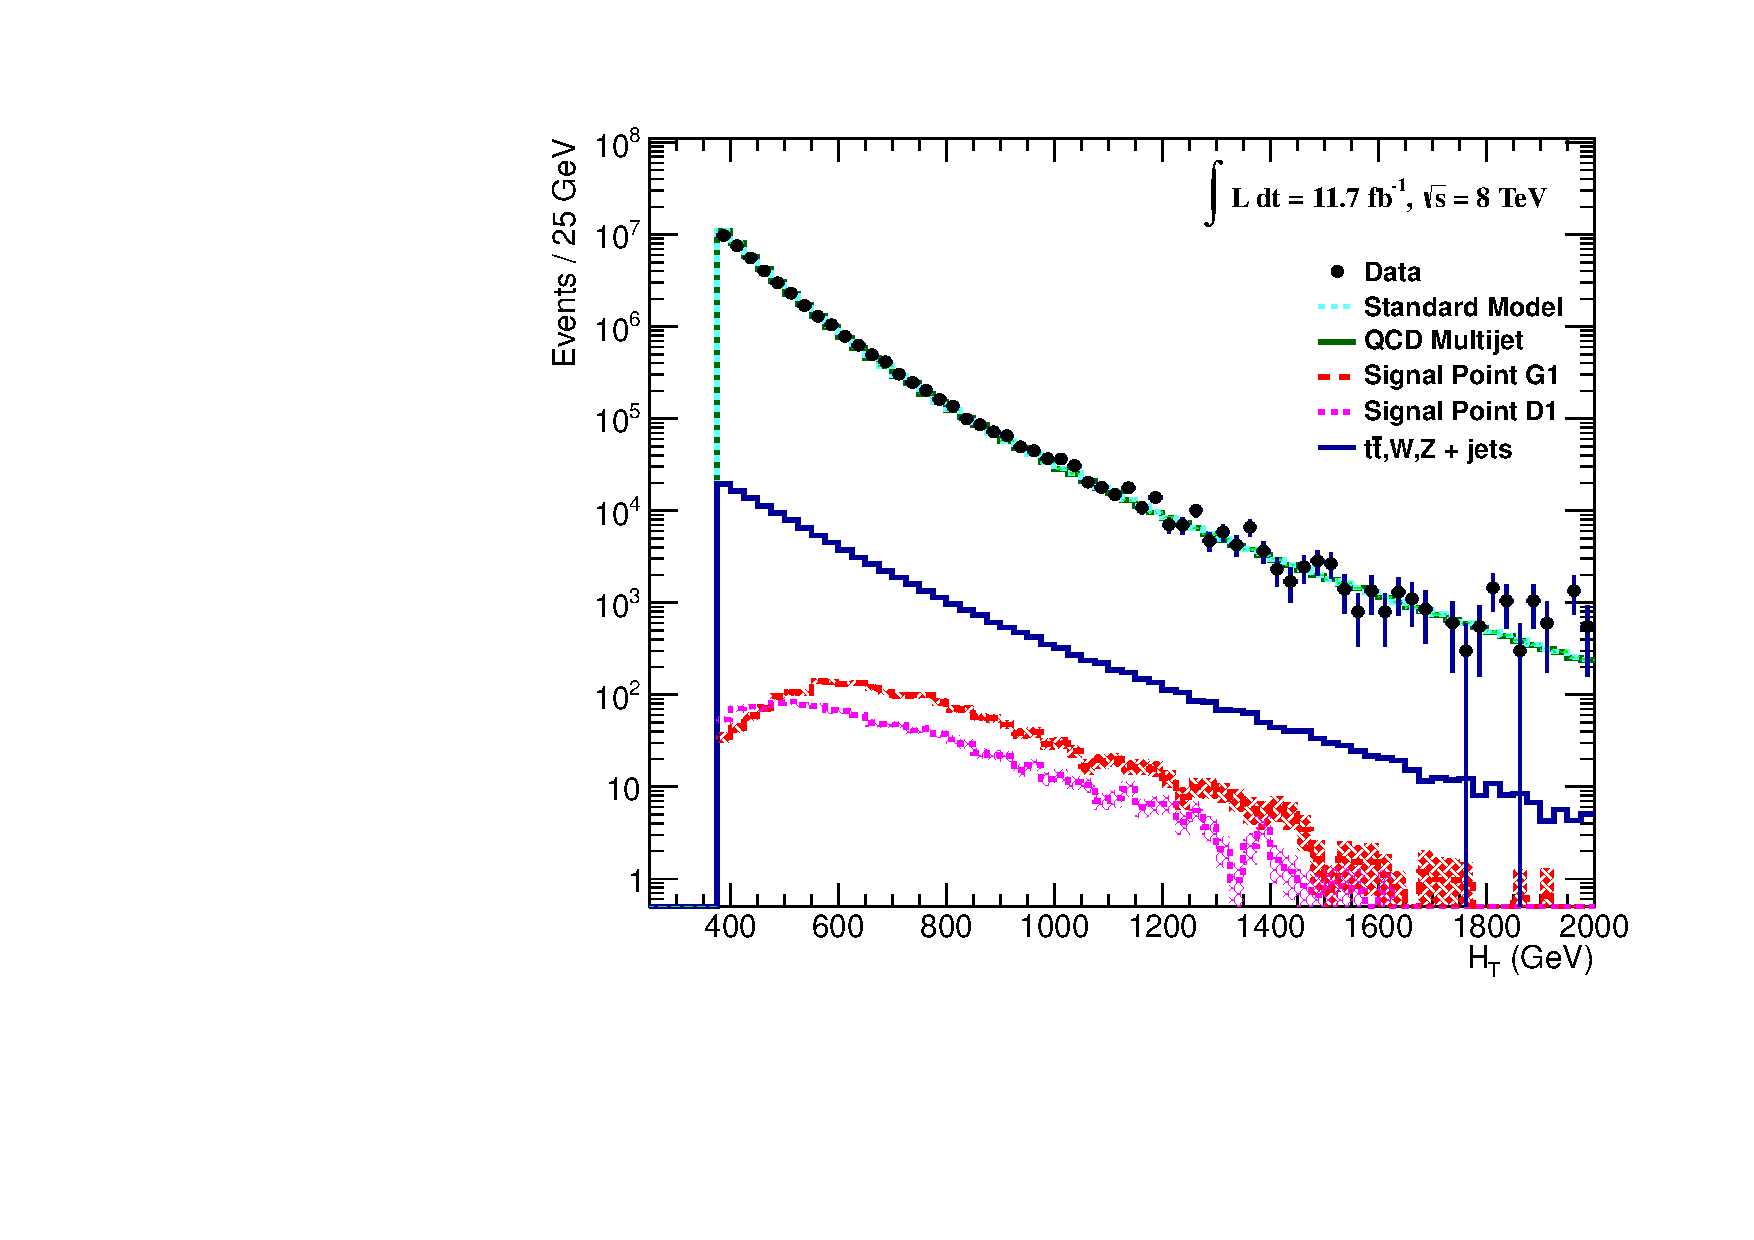
\includegraphics[width=0.70\textwidth]{plots/ra1_htdistribution.pdf}
\caption[Reconstructed offline $\theht$ distribution in the hadronic signal selection (detailed in the following section), from 11.7fb$^{-1}$ of data, in which no \alphat requirement was made.]{Reconstructed offline $\theht$ distribution in the hadronic signal selection (detailed in the following section), from 11.7fb$^{-1}$ of data, in which no \alphat requirement was made. The sample is collected from prescaled \theht triggers. Overlaid are expectations from simulation of \ac{EWK} processes as well as two reference signal models (labelled G1 and D1 from Table \ref{tab:sms_model_table}).}  
\label{fig:htqcdbackground}
\end{figure}

Additional \ac{SM} background from \ac{EWK} processes with genuine $\met$ from escaping neutrinos comprise the irreducible background within this search and come mainly from:

\begin{itemize}
\item $Z \rightarrow \nu\bar{\nu}$ +  jets,
\item $W \rightarrow l\nu$ + jets in which a lepton falls outside of detector acceptance, is not reconstructed, is mis-identified, or the lepton decays hadronically $\tau \rightarrow$ had,
\item $t\bar{t}$ with at least one leptonically decaying W, which is missed in the detector as detailed above,
\item small background contributions from DY, single top and Diboson (WW,ZZ,WZ) processes.
\end{itemize}

The search is designed to have a strong separation between events with genuine and ``fake'' $\met$ which is achieved primarily though the dimensionless kinematic variable, $\alphat$ \cite{alphat7tev}\cite{CMS:2008vya}.

\subsection{The $\alphat$ Variable}
\label{subsec:alphatvariable}

For a perfectly measured di-jet QCD event, conservation laws dictate that both jets must be of equal magnitude and produced in opposite directions. However, in the case of di-jet events with genuine $\met$ (as detailed above), no such requirement is made of the two jets, as depicted in Figure \ref{fig:susytopology}.
\begin{figure}[!h]
\centering
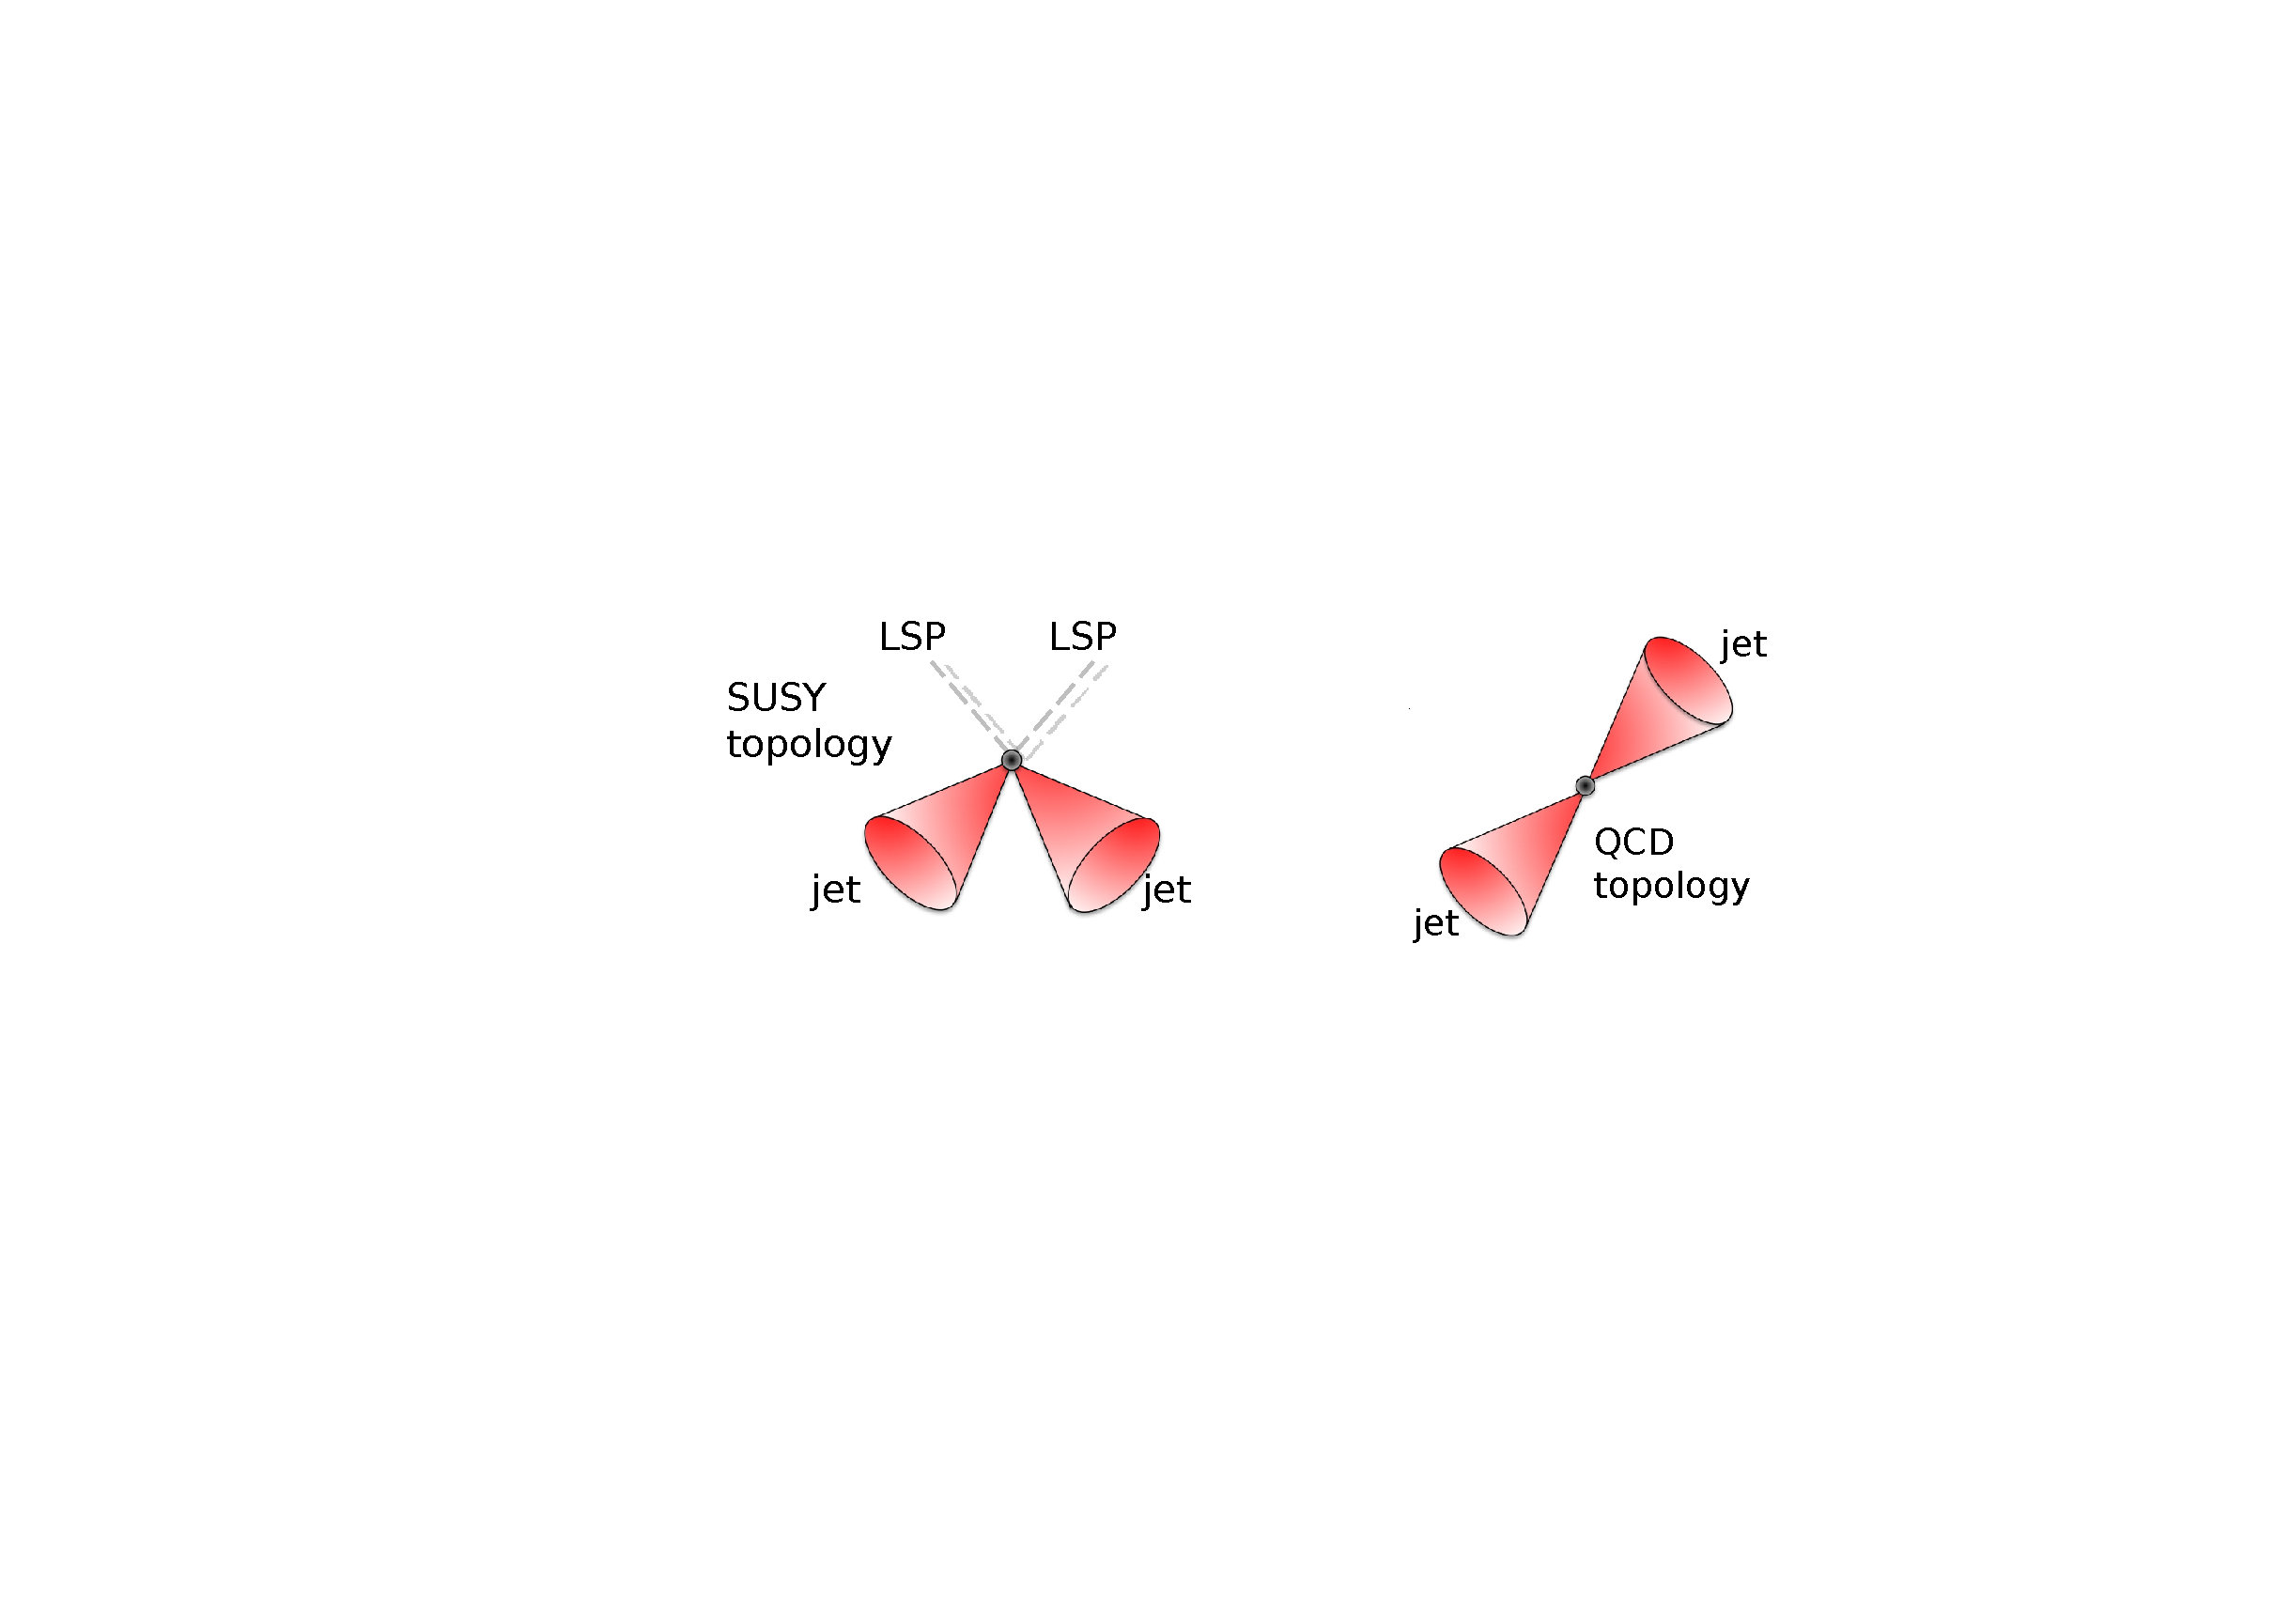
\includegraphics[width=0.90\textwidth]{plots/susy_topology.pdf}
\caption[The event topologies of background QCD diet events (right) and a generic \ac{SUSY} signature with genuine $\met$ (left).]{The event topologies of background QCD diet events (right) and a generic \ac{SUSY} signature with genuine $\met$ (left).}  
\label{fig:susytopology}
\end{figure}

 Exploiting this feature leads to the formulation of $\alphat$ (first inspired by \cite{PhysRevLett.101.221803}) in di-jet systems defined as,

\begin{equation}
\alphat = \frac {E^{j_{2}}_{T}}{M_{T}},
\end{equation} 

where $E^{j_{2}}_{T}$ is the transverse energy of the least energetic of the two jets and $M_{T}$ defined as:

\begin{equation}
\label{eq:transmass}
M_{T} = \sqrt{\left(\sum^{2}_{i=1}E^{j_{i}}_{T}\right)^{2}-\left(\sum^{2}_{i=1}p^{j_{i}}_{x}\right)^{2}-\left(\sum^{2}_{i=1}p^{j_{i}}_{y}\right)^{2}} \equiv \sqrt{H_{T}^{2} - \mht^{2}} .
\end{equation}

A perfectly balanced di-jet event i.e. $E_{T}^{j_{1}} = E_{T}^{j_{2}}$ would yield an \alphat value of 0.5. In processes where a W or Z recoils off a system of jets, these jets will not necessarily be perfectly balanced and $\alphat$ can then achieve values in excess of 0.5. Most importantly, balanced multi-jet events in which jets \emph{are} mis-measured, will generally result in an \alphat value of less than 0.5, thus giving the \alphat variable discriminating power between these processes.

$\alphat$ can be further extended to apply to any arbitrary number of jets. This is undertaken by modelling a system of $n$ jets as a di-jet system, through the formation of two pseudo-jets \cite{CMS-PAS-SUS-09-001}. The two pseudo-jets are built by merging the jets present, and are chosen to be as balanced as possible, i.e the $\Delta$\theht $\equiv \lvert E_{T}^{pj_{1}} - E_{T}^{pj_{2}}\rvert$ is minimised between the two pseudo jets. Using Equation (\ref{eq:transmass}), $\alphat$ can be rewritten as,

\begin{equation}
\label{eq:alphatmht}
\alphat = \frac{1}{2} \frac {\theht - \Delta\theht}{\sqrt{\theht^{2}-\mht^{2}}}= \frac{1}{2}\frac{1-\Delta\theht/\theht}{\sqrt{1-(\mht/\theht)^{2}}}.
\end{equation}

The distribution of $\alphat$ for the two jet multiplicity categories used within this analysis, 2$\leq n_{jet} \leq$3 and $ n_{jet} \geq 4$ jets, is shown in the Figure \ref{fig:fullalphatdistribution}. It can be seen that the distributions peak at an \alphat value of 0.5, before falling away sharply and being free of a simulated multi-jet background at larger \alphat values. These distributions serve to demonstrate the ability of the $\alphat$ variable to discriminate between multi-jet events and \ac{EWK} processes with genuine $\met$ in the final state. 

\begin{figure}[ht]
\centering
\begin{minipage}[b]{0.48 \linewidth}
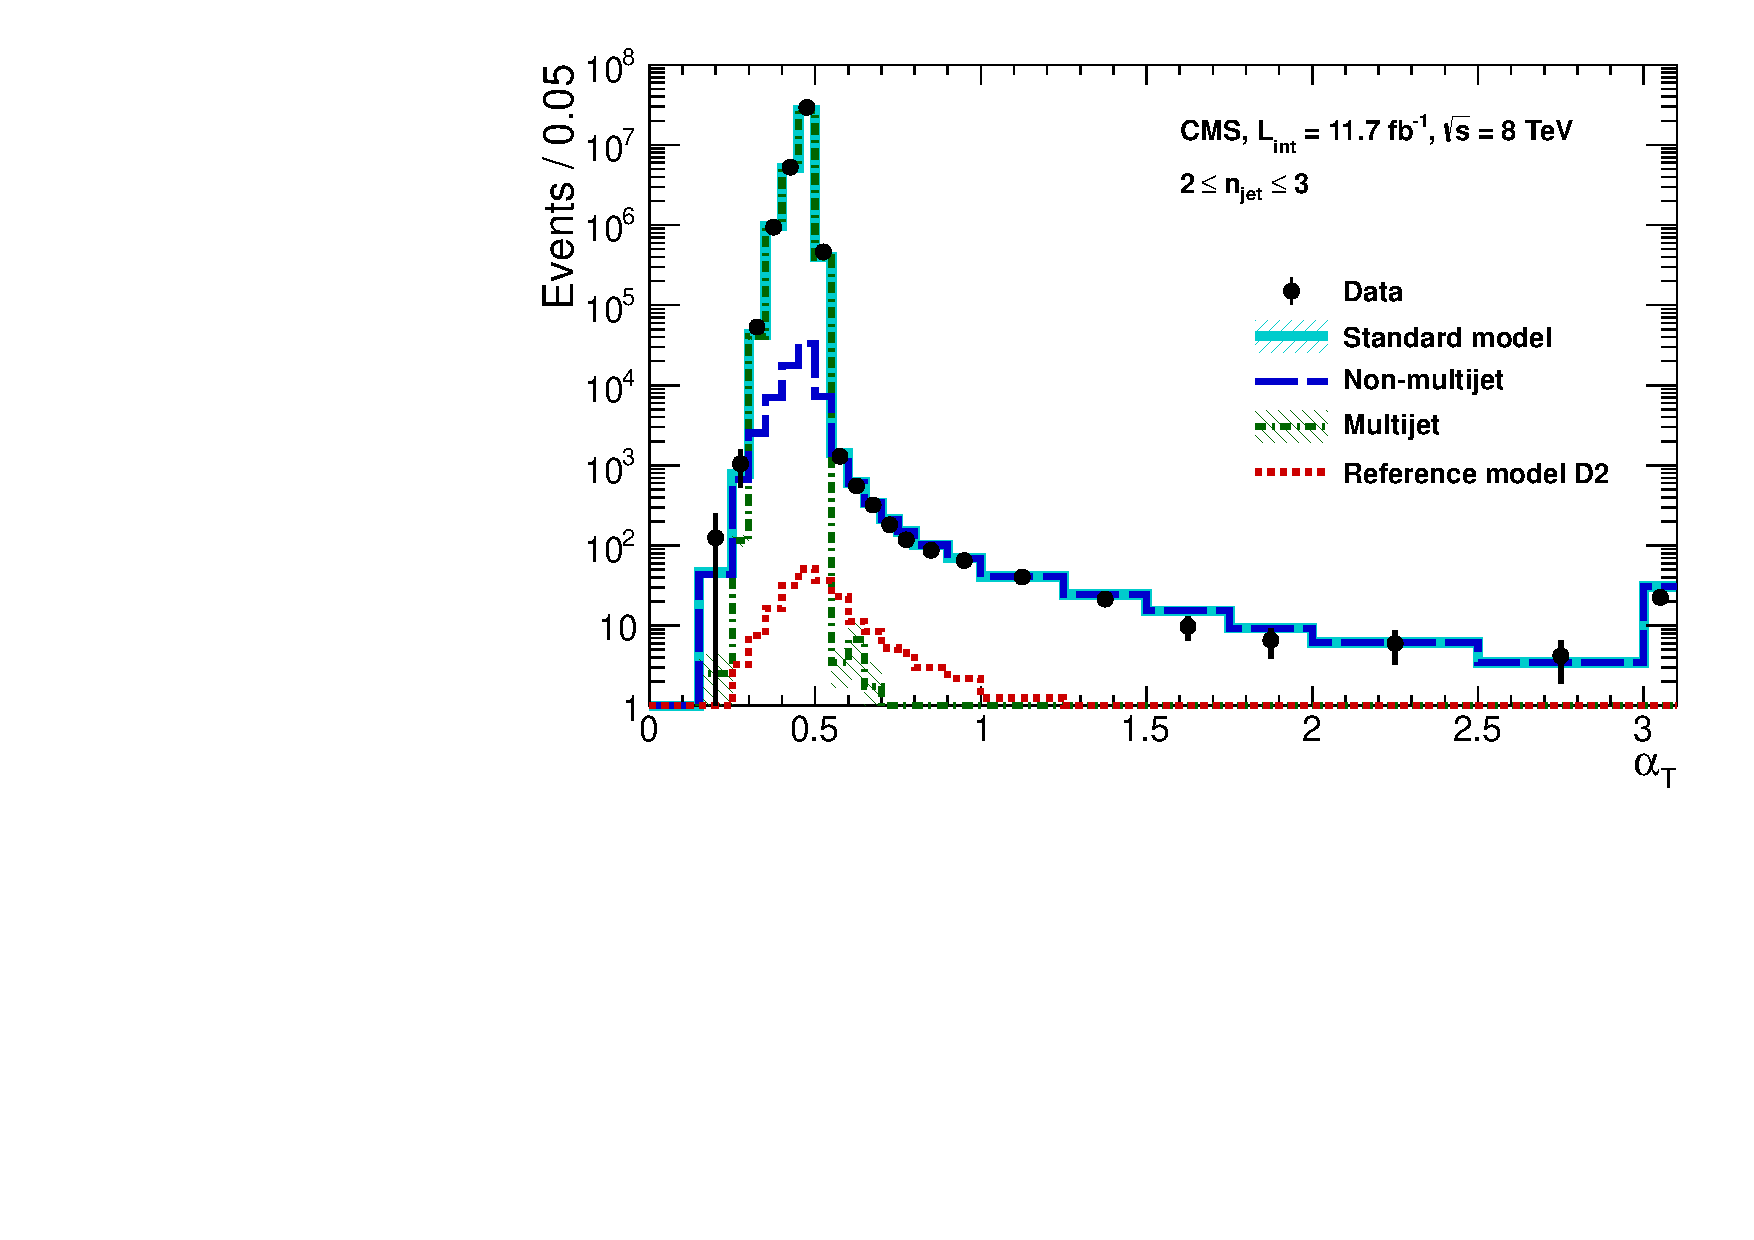
\includegraphics[width = 1.0\linewidth,height = 7.0cm]{plots/alphat_low.pdf}
\end{minipage}
\quad
\begin{minipage}[b]{0.48\linewidth}
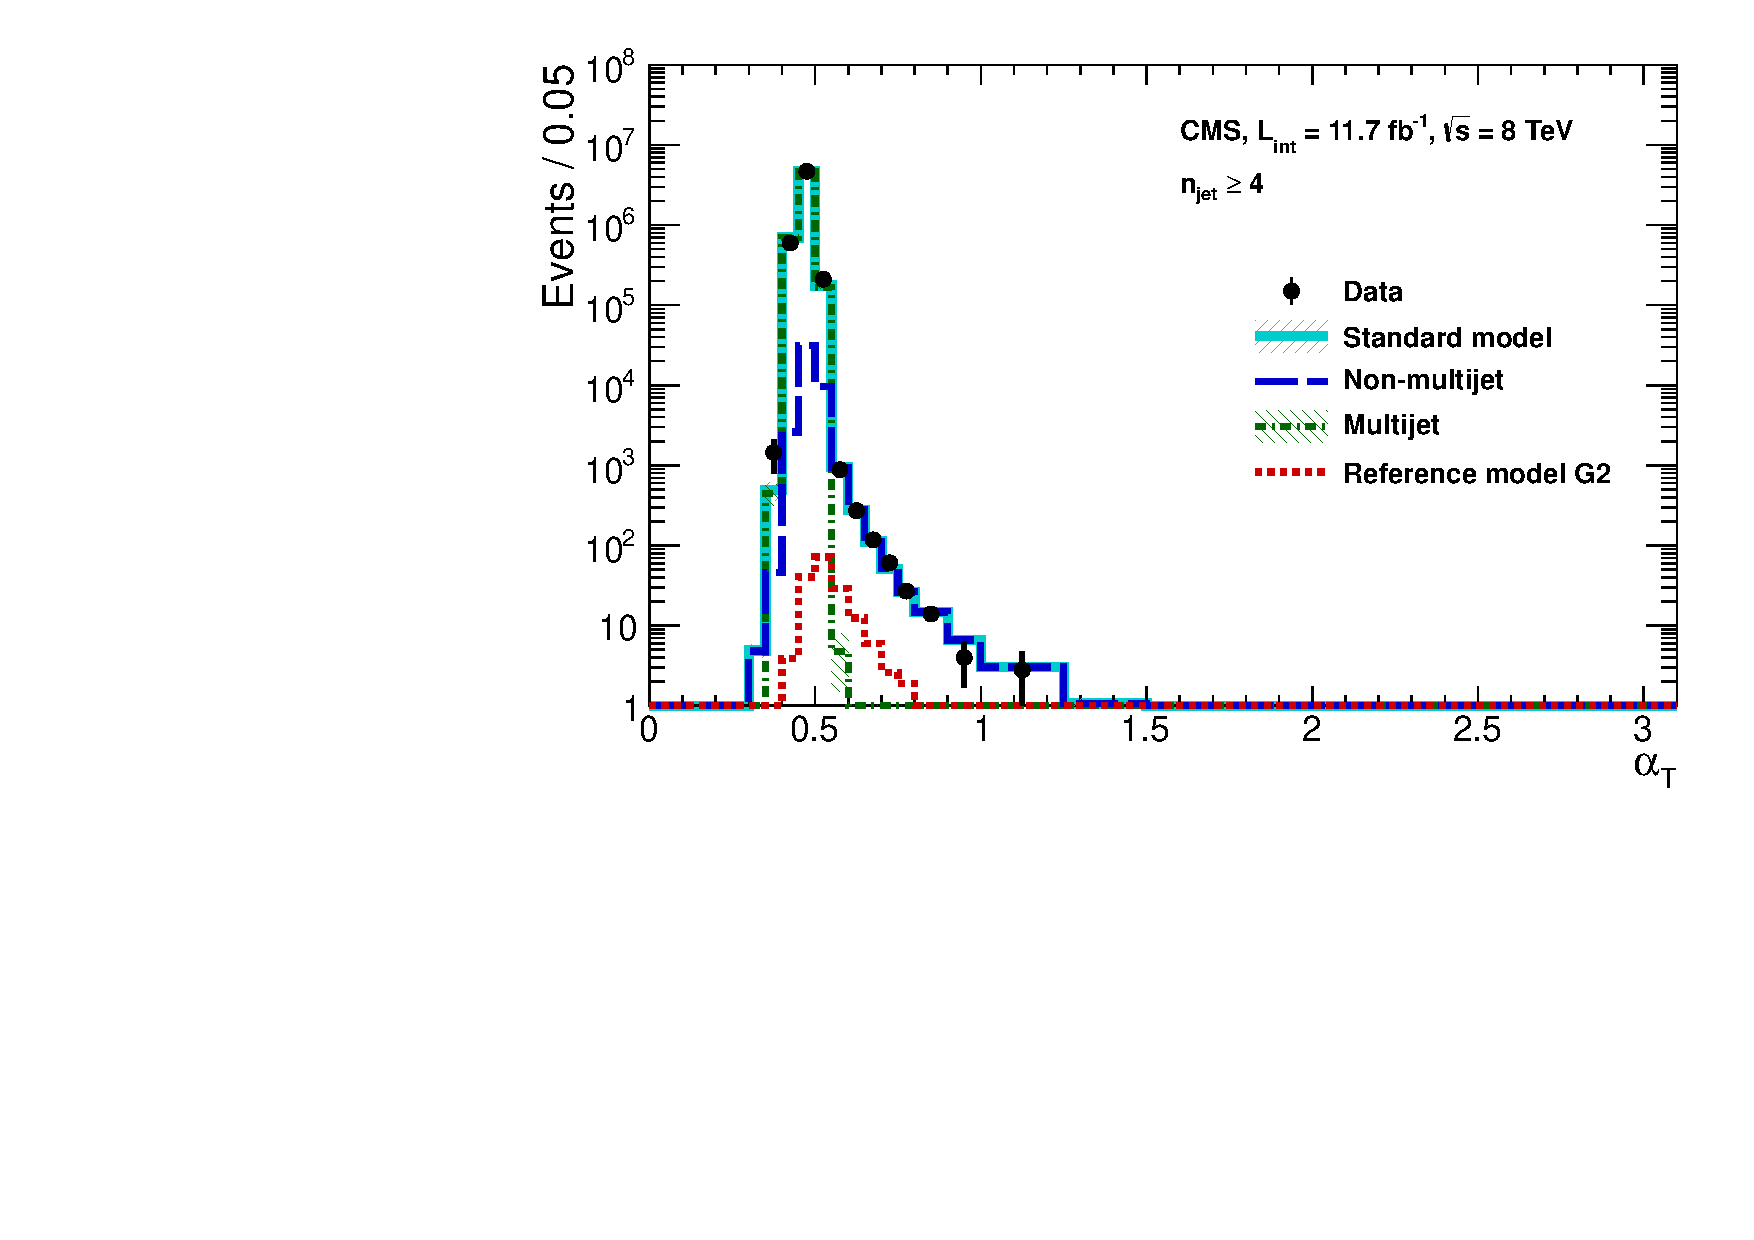
\includegraphics[width = 1.0\linewidth, height = 7.0cm]{plots/alphat_high.pdf}
\end{minipage}
\caption[ The $\alphat$ distributions for the low 2-3 (left) and high $\geq 4$ (right) jet multiplicities after a full analysis selection and $\theht > 375$ requirement.]{The $\alphat$ distributions for the low 2-3 (left) and high $\geq 4$ (right) jet multiplicities after a full analysis selection and $\theht > 375$ requirement. Data is collected using both prescaled $\theht$ triggers and dedicated $\alphat$ triggers for below and above $\alphat = 0.55$ respectively. Expected yields as given by simulation are also shown for multi-jet events (green dash-dotted line), \ac{EWK} backgrounds with genuine $\met$ (blue long-dashed line), the sum of all \ac{SM} processes (cyan solid line) and the reference signal model D2 (left, red dotted line) or G2 (right, red dotted line). }
\label{fig:fullalphatdistribution}
\end{figure}

The $\alphat$ requirement used within the search is chosen to be $\alphat >$ 0.55 to ensure that the QCD multi-jet background is negligible even in the presence of moderate jet mis-measurement. There still remain other effects which can cause multi-jet events to artificially have a large $\alphat$ value, methods to combat them are discussed in detail in Section (\ref{subsec:eventselection}).  


\section{Search Strategy}
\label{subsec:searchstrategy}

The aim of the analysis presented in this thesis is to identify an excess of events in data over the \ac{SM} background expectation in multi-jet final states and significant $\met$. The essential suppression of the dominant multi-jet background for such a search is addressed by the $\alphat$ variable, described in the previous section. For estimation of the remaining \ac{EWK} backgrounds, three independent data control samples are used to predict the different processes that compose the background :

\begin{itemize}
\item \mupjets control sample to determine W + jets, \ttbar and single top backgrounds,
\item \gpjets control sample to determine the irreducible \zinv + jets background,
\item \dimupjets control sample to also determine the irreducible \zinv + jets background.
\end{itemize}

These control samples are chosen to be rich in specific \ac{EWK} processes, free of QCD multi-jet events and to also be kinematically similar to the hadronic signal region that they are estimating the backgrounds of, see Section (\ref{subsec:controlsampledefinition}). The redundancy of using the \gpjets and \dimupjets sample to predict the same background within the signal region, brings an opportunity to reliably crosscheck and validate the background estimation method, and is utilised in both the determination of background estimation systematics (Section(\ref{subsec:sysuncertainties})) and in the maximum likelihood fit (Section(\ref{sec:statframework})).

To remain inclusive to a large range of possible \ac{SUSY} models, the signal region is split into the following categories to allow for increased sensitivity to different \ac{SUSY} topologies:

\begin{itemize}

\item[] \textbf{Sensitivity to a range of \ac{SUSY} mass splittings}

The hadronic signal region is defined by \theht $>$ 275, divided into eight bins in \theht. 

\begin{itemize}
\item Two bins of width 50 \GeV in the range 275 $<$ \theht $<$ 375 \GeV,
\item five bins of width 100 \GeV in the range 375 $<$ \theht$<$ 875 \GeV,
\item and a final open bin, \theht $>$ 875 \GeV.
\end{itemize}

The choice of the lowest \theht bin in the analysis is driven primarily by trigger constraints. The mass difference between the \ac{LSP} and the particle that it decays from is an important factor in the amount of hadronic activity in the event. 

A large mass splitting will lead to hard high \pt jets which contribute to the \theht sum. From Figure \ref{fig:htqcdbackground} it can be seen that the \ac{SM} background falls sharply at high \theht values, therefore many \theht categories will lead to easier identification of such signals. Conversely, smaller mass splittings lead to softer jet \pt's which will subsequently fall into the lower \theht range.

\item[] \textbf{Sensitivity to production method of \ac{SUSY} particles}

The production mechanism of any potential \ac{SUSY} signal can lead to different event topologies. One such way to discriminate between gluino ($g\widetilde{g}$ - ``high multiplicity''), and direct squark ($q\widetilde{q}$ - ``low multiplicity'') induced production of \ac{SUSY} particles is realised through the number of reconstructed jets in the final state.  

The analysis is thus split into two jet categories: 2 $\leq \njet \leq$ 3 jets, $\njet \geq$ 4 jets to give sensitivity to both of these mechanisms. 

\item[] \textbf{Sensitivity to  ``Natural \ac{SUSY}'' via tagging jets from b-quarks}

Jets originating from the hadronisation of bottom quarks (b-jets) are identified through vertices that are displaced with respect to the primary interaction. The algorithm used in the analysis to identify b-jets is the \acf{CSVM} tagger, described within Section (\ref{subsec:cmsobjects-btagging}). A cut is placed on the discriminator variable of $> 0.679$, leading to a gluon/light-quark tagging efficiency of $\sim$ 1\%, a c-quark tagging efficiency of $\sim$ 20\% and a jet p$_{\text{T}}$ dependant b-tagging efficiency of 60-70\% \cite{btagscalefactor}.

Natural \ac{SUSY} models would be characterised through final-state signatures rich in bottom quarks. A search relying on methods to identify jets originating from bottom quarks through b-tagging, will significantly improve the sensitivity to this class of signature. This gain in sensitivity stems from a vast reduction in the vector boson + jet backgrounds (W, Z) at higher b-tag jet multiplicities, which typically have no b-flavoured quarks in their decays.  

Therefore, events are categorised according to the number of offline reconstructed b-tagged jets, \nbreco, identified within each event. The following five categories are used; \nbreco =0, =1, =2, =3 and $\geq$ 4. In the \nbreco $\geq$ 4 category, due to a limited number of expected signal and background events just three \theht bins are employed: 275-325 \GeV, 325-375 \GeV, $\geq$ 375 \GeV.

This characterisation is identically mirrored in all control samples, with the information from all samples and b-tag categories used simultaneously in the likelihood model, see Section (\ref{sec:statframework}).

\end{itemize}
 
 The combination of the \theht, jet multiplicity and b-tag categorisation of the signal region as described above, results in 67 different bins in which the analysis is interpreted in. A visualisation of the analysis categorisation is depicted in Figure \ref{fig:analysisbinning}. 
 
 \begin{figure}[!h]
 \centering
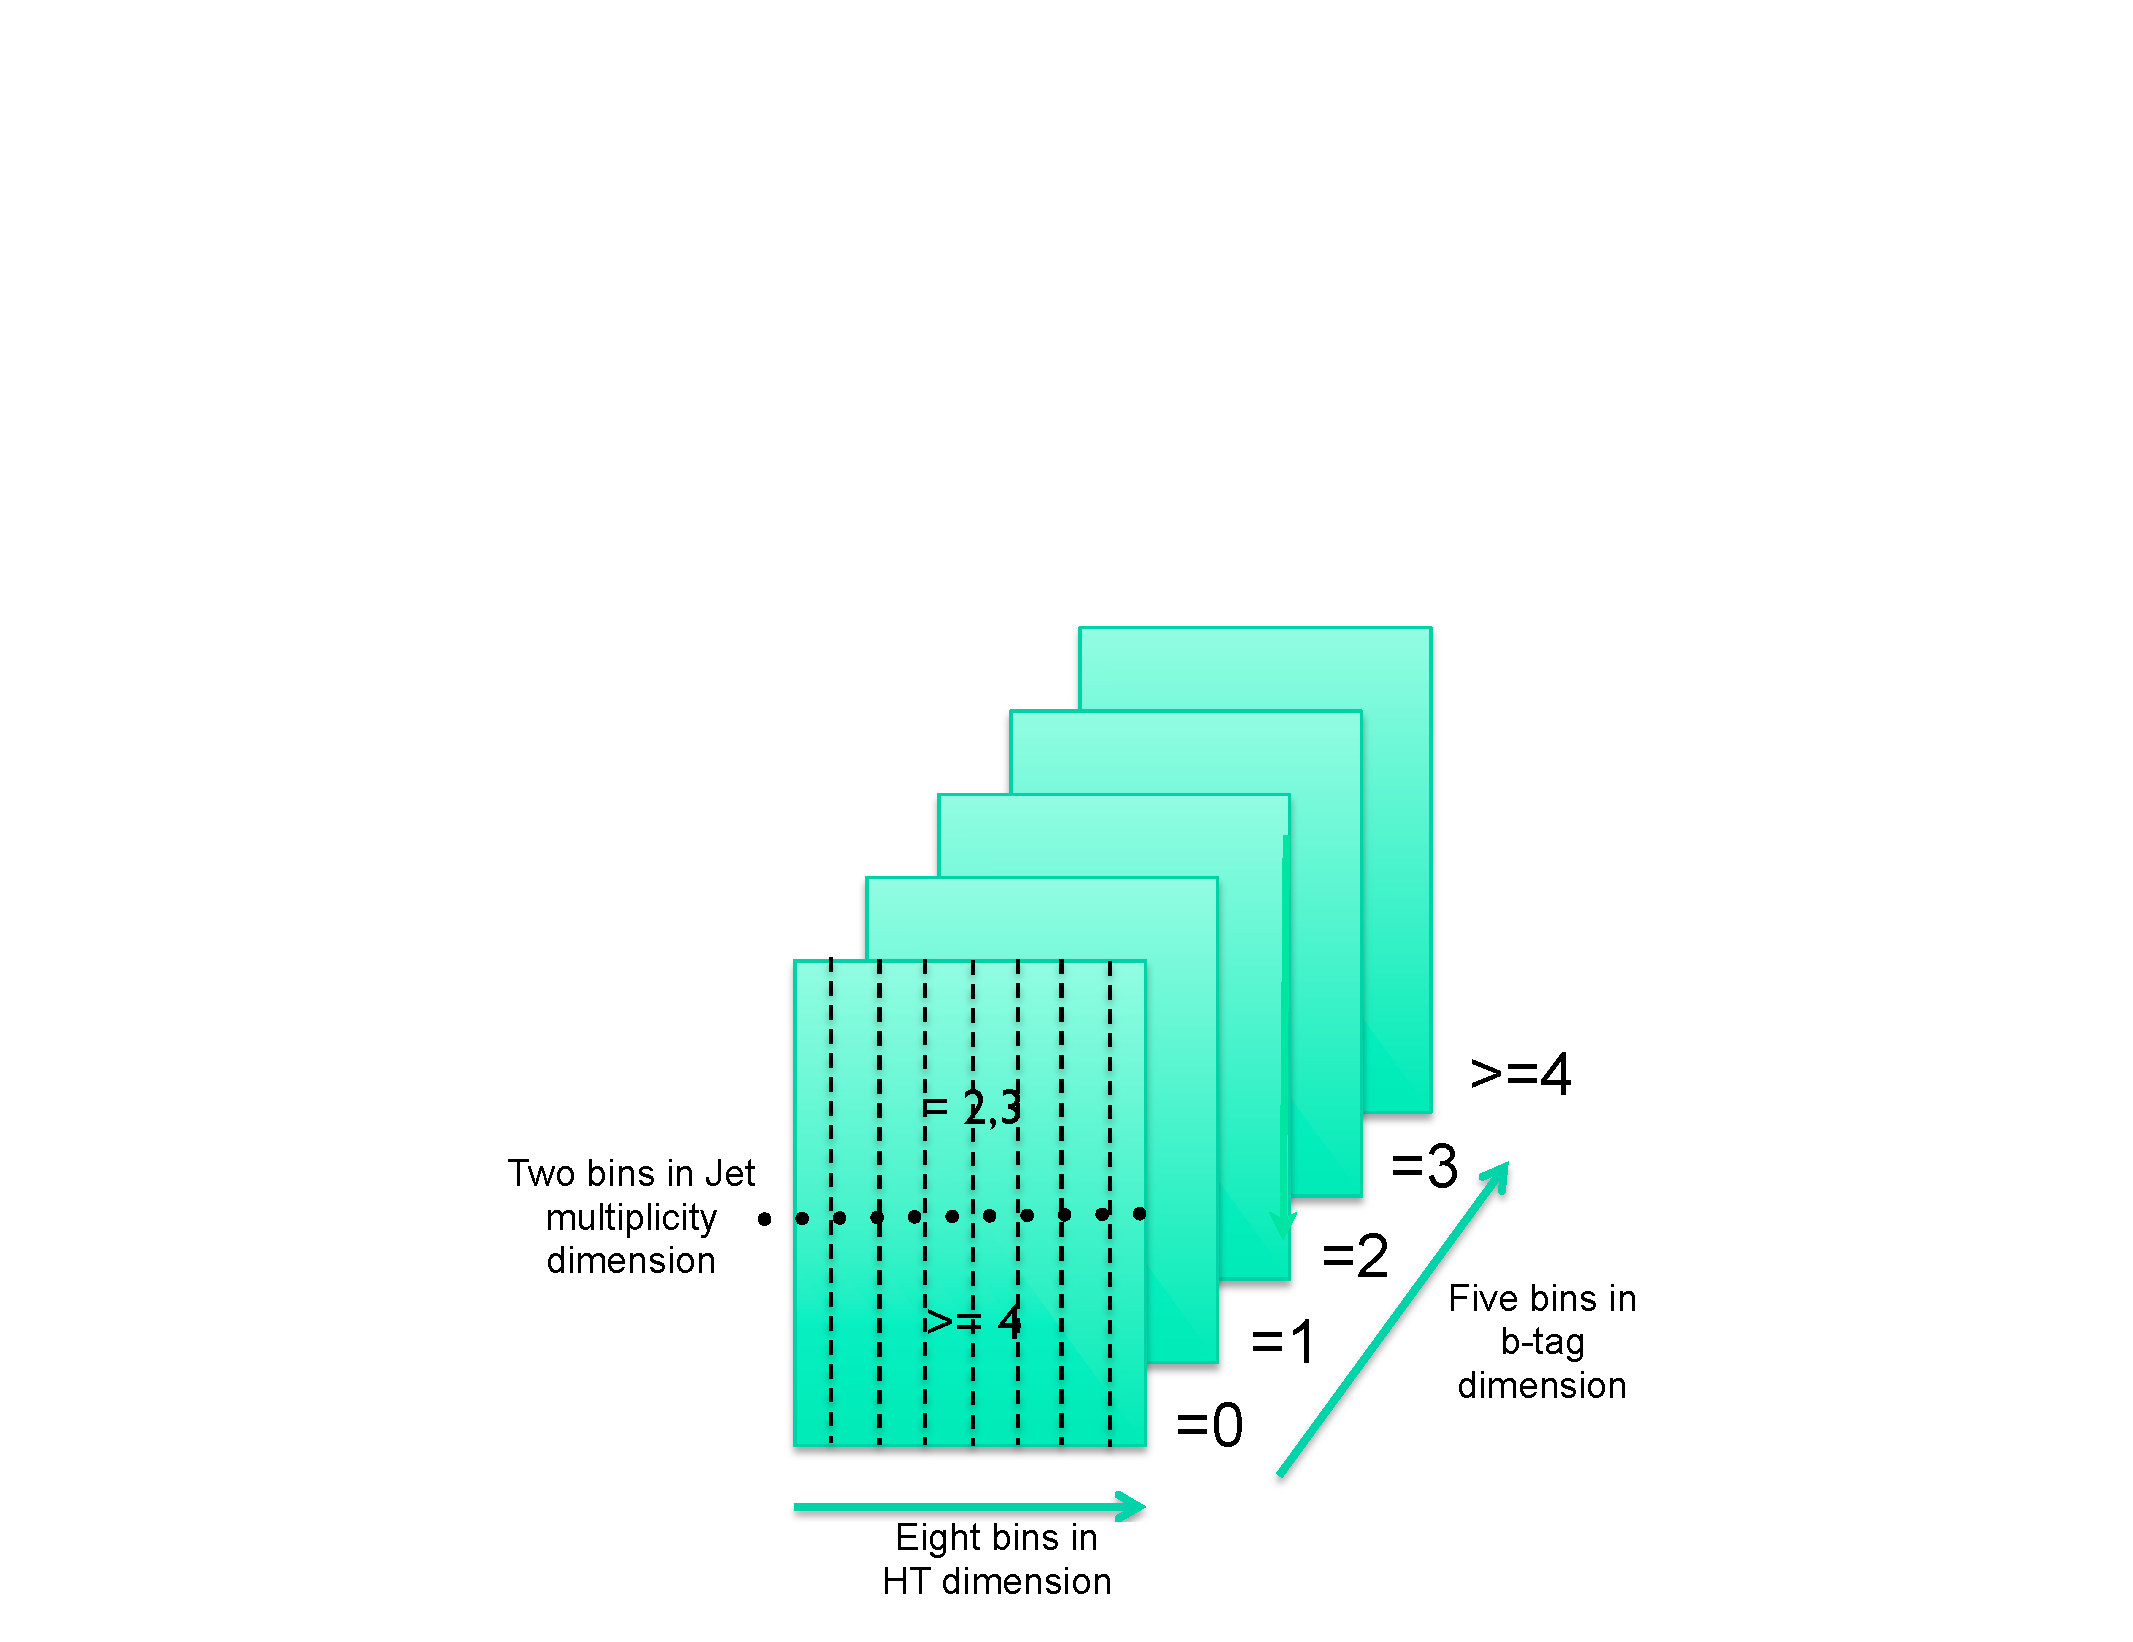
\includegraphics[width=0.70\textwidth]{plots/analysis_binning.pdf}
\caption[Pictorial depiction of the analysis strategy employed by the $\alphat$ search to increase sensitivity to a wide spectra of \ac{SUSY} models.]{Pictorial depiction of the analysis strategy employed by the $\alphat$ search to increase sensitivity to a wide spectra of \ac{SUSY} models.}  
\label{fig:analysisbinning}
\end{figure}
\FloatBarrier
\subsection{Physics Objects}
\label{subsec:physicsobjects}

The physics objects used in the analysis are defined below, and follow the recommendation of the various \ac{CMS} \acf{POGs}. 

\begin{itemize}

\item \textbf{Jets}

The jets used in this analysis are CaloJets, reconstructed as described in Section (\ref{subsec:cmsobjects-jets}) using the anti-k$_{T}$ jet clustering algorithm. 

To ensure the jet object falls within the calorimeter systems a pseudo-rapidity requirement of \abeta $<$ 3 is applied. Each jet must pass a ``loose'' identification criteria to reject jets resulting from unphysical energy, the criteria of which are detailed in Table \ref{tabapp:calojetid} \cite{CMS-PAS-JME-09-008}.

\item \textbf{Muons}

Muons are selected in the \mupjets and \dimupjets control samples, and vetoed in the signal region. The same cut based identification criteria is applied to muons in both search regions and is summarised in Table \ref{tab:muonidtable} \cite{2012JInst...7P0002T}.

\begin{table}[h!]
\footnotesize
\begin{center}
\begin{tabulary}{0.98\textwidth}{LL}
\cline{1-2}
Variable & Definition \\ 
\hline\hline
Is Global Muon \qquad\qquad\qquad\qquad\qquad\qquad\qquad\qquad\qquad\qquad& Muon contains both a hit in the muon chamber and a matched track in the inner tracking system.\\
$\chi^{2}$$<$ 10 & $\chi^{2}$ of global muon track fit. Used to suppress hadronic punch-through and muons from decays in flight.  \\
Muon chamber hits $>$ 0 &  At least one muon chamber hit included in global muon track fit.\\
Muon station hits $>$ 1 & Muon segment hits in at least two muon stations, which  suppresses hadronic punch-through and accidental track-to-segment matches. \\
d$_{xy} <$ 0.2mm & The tracker track transverse impact parameter w.r.t the primary vertex. Suppresses cosmic muons and muons from decays in flight. \\
d$_{z} <$ 0.5mm & The longitudinal distance of the tracker track w.r.t the primary vertex. Loose selection requirement to further suppress cosmic muons, muons from decays in flight and tracks from pileup.\\
Pixel hits $>$ 0 & Suppresses muons from decays in flight by requiring at least one pixel hit in the tracker. \\
Track layer hits $>$ 5 & Number of tracker layers with hits, to guarantee a good \pt measurement. Also suppresses muons from decays in flight.\\
PF Iso  $<$0.12 & Isolation based upon the sum of the charged and neutral hadrons and photon objects within a $\Delta$R 0.4 cone of the muon object, corrected for pile up effects on the isolation sum.   \\
\cline{1-2}
\end{tabulary}
\end{center}
\caption[Muon identification criteria used within the analysis for selection/veto purposes in the muon control/signal selections.]{Muon identification criteria used within the analysis for selection/veto purposes in the muon control/signal selections.}
\label{tab:muonidtable}
\end{table}
\FloatBarrier
Additionally muons are required to be within the acceptance of the muon tracking systems. For the muon control samples, trigger requirements necessitate a \abeta $<$ 2.1 for the selection of muons. In the signal region where muons are vetoed, these conditions are relaxed to  \abeta $<$ 2.5 and a minimum threshold of \pt $> 10 $ \GeV is required of muon objects. 

\item \textbf{Photons} 

Photons are selected within the \gpjets control sample and vetoed in all other selections. Photons are identified in both cases according to the cut based criteria listed in Table \ref{tab:photonidtable} \cite{CMS-PAS-SUS-12-018}.

\setlength\LTleft{1.5cm}
\setlength\LTright{\LTleft}
\begin{footnotesize}
\begin{center}
\begin{longtable}{@{\extracolsep{\fill}}p{2.0cm}p{10cm}}

\hline \multicolumn{2}{r}{\textit{Continued on next page}} \\ 
\endfoot

\endlastfoot
\hline
Variable & Definition \\ 
\hline\hline \\
H/E $< $ 0.05  \qquad\qquad\qquad\qquad\qquad\qquad & The ratio of hadronic energy in the \ac{HCAL} tower directly behind the \ac{ECAL} super-cluster and the \ac{ECAL} super-cluster itself. \\
$\sigma_{i\eta i\eta}< 0.011$ \qquad\qquad\qquad\qquad\qquad\qquad\qquad\qquad  & The log energy weighted width ($\sigma$), of the extent of the shower in the $\eta$ dimension.\\
R9 $<$ 1.0 & The ratio of the energy of the 3$\times$3 crystal core of the super-cluster compared to the total energy stored in the 5$\times$5 super-cluster. \\
Combined Isolation $<$ 6 \GeV &  The photons are required to be isolated with no electromagnetic or hadronic activity within a radius $\Delta$R = 0.3 of the photon object. A combination of the pileup subtracted \cite{Cacciari:2007fd}, \ac{ECAL}, \ac{HCAL} and tracking isolation sums are used to determine the combined total isolation value.  \\
\hline
\caption[Photon identification criteria used within the analysis for selection/veto purposes in the \gpjets control/signal selections. ]{Photon identification criteria used within the analysis for selection/veto purposes in the \gpjets control/signal selections.}
\label{tab:photonidtable}
\end{longtable}
\end{center}
\end{footnotesize}

\FloatBarrier
Photon objects are also required to have a minimum momentum of \pt $>$ 25 \GeV.

\item \textbf{Electrons}

Electron identification is defined for veto purposes. They are selected according to the following cut-based criteria listed in Table \ref{tab:electronidtable}, utilising PF-based isolation.

\begin{table}[h!]
\footnotesize
\begin{center}
\begin{tabulary}{1.0\textwidth}{LCCL}
\cline{1-4}
Variable & Barrel &  EndCap & Definition\\ 
\hline\hline
$\Delta \eta_{In}$ \qquad\qquad\qquad\qquad\qquad\qquad\qquad\qquad\qquad\qquad\qquad\qquad & $<$0.007 \qquad\qquad\qquad\qquad\qquad & $<$0.009 \qquad\qquad\qquad\qquad\qquad\qquad& $\Delta\eta$ between SuperCluster position and the coordinate of the associated track at the interaction vertex, assuming no radiation. \\
$\Delta \phi_{In}$ & $<$0.15 & $<$0.10 & $\Delta\phi$ between SuperCluster position and track direction at interaction vertex extrapolated to ECAL assuming no radiation. \\
$\sigma_{i\eta i\eta}$ & $<$0.01 & $<$0.03 & Cluster shape covariance, measure the $\eta$ dispersion of the electrons electromagnetic shower over the  \ac{ECAL} supercluster. \\
H/E & $<$0.12 & $<$0.10 & The ratio of hadronic energy in the \ac{HCAL} tower directly behind the \ac{ECAL} super-cluster and the \ac{ECAL} super-cluster itself.\\
d0 (vtx) & $<$0.02 & $<$0.02 & The tracker track transverse impact parameter w.r.t the primary vertex.  \\
dZ (vtx) & $<$0.20 & $<$0.20 & The longitudinal distance of the tracker track w.r.t the primary vertex.\\
$\lvert(\frac{1}{E_{ECAL}} - \frac{1}{p_{track}})\rvert$ & $<$0.05 & $<$0.05 & Comparison of energy at supercluster 1/E$_{ECAL}$ and that of the track momentum at the vertex 1/p$_{track}$. Causes suppression of fake electrons at low \pt. \\
PF Iso & $<$0.15 & $<$0.15 & Combined PF isolation of charged hadrons, photons, neutral hadrons within a $\Delta$R $<$ 0.3 cone size. Isolation sum is corrected for pileup using effective area corrections for neutral particles. \\
\cline{1-4}
\end{tabulary}
\end{center}
\caption[Electron identification criteria used within the analysis for veto purposes.]{Electron identification criteria used within the analysis for veto purposes.}
\label{tab:electronidtable}
\end{table}

Electrons are required to be identified at \abeta $<$ 2.5, with a minimum \pt $>$ 10 \GeV threshold to ensure that the electrons fall within the tracking system of the detector.

\FloatBarrier

\item \textbf{Noise and \met Filters}

A series of noise filters are applied to veto events which contain spurious non-physical jets that are not picked up by the jet id, and events which give large unphysical \met values. These filters are listed within Table \ref{tab:noiseid}.

\begin{table}[h!]
\footnotesize
\begin{center}
\begin{tabulary}{0.80\textwidth}{p{4cm}L}
\cline{1-2}
\multicolumn{2}{l}{Noise Filters} \\
Variable & Definition \\ 
\hline\hline
 CSC tight beam halo filter \qquad\qquad\qquad\qquad\qquad & As proton beams circle the \ac{lhc}, proton interactions with the residual gas particles or the beam collimators can occur, producing showers of secondary particles which can interact with the \ac{CMS} detector. \\
 HBHE noise filter with isolated noise rejection & Anomalous noise in the \ac{HCAL} not due to electronics noise, but rather due to instrumentation issues associated with the \ac{HPD}'s and \acf{RBXs}. \\
 HCAL laser filter & The \ac{HCAL} uses laser pulses for monitoring the detector response. Some laser pulses have accidentally been fired in the physics orbit, and ended up polluting events recorded for physics analysis. \\
 ECAL dead cell trigger primitive (TP) filter & \ac{EB} and \ac{EE} have single noisy crystals which are masked in reconstruction. Use the \acf{TP} information to assess how much energy was lost in masked cells. \\
 Bad EE Supercrystal filter & Two supercrystals in \ac{EE} are found to occasionally produce high amplitude anomalous pulses in several channels at once, causing a large \met spike. \\
 ECAL Laser correction filter & A laser calibration multiplicative factor is applied to correct for transparency loss in each crystal during irradiation. A small number of crystals receive unphysically large values of this correction and become very energetic, resulting in \met. \\
\cline{1-2}
\end{tabulary}
\end{center}
\caption[Noise filters that are applied to remove spurious and non-physical \met signatures within the \ac{CMS} detector.]{Noise filters that are applied to remove spurious and non-physical \met signatures within the \ac{CMS} detector.}
\label{tab:noiseid}
\end{table}  


\end{itemize}

\FloatBarrier

\subsection{Event Selection}
\label{subsec:eventselection}

The selection criteria for events within the analysis are detailed below. A set of common cuts are applied to both signal  (maximise acceptance to a range of \ac{SUSY} signatures),  and control samples (retain similar jet kinematics for background predictions), with additional selection cuts applied to each control sample to enrich the sample in a particular \ac{EWK} processes, see Section (\ref{subsec:controlsampledefinition}).

The jets considered in the analysis are required to have a transverse momentum \pt $>$ 50 \GeV, with a minimum of two jets required in the event. The highest \et jet is required to lie within the central tracker acceptance \abeta $<$ 2.5, and the two leading \pt jets must each have \pt $>$ 100 \GeV.  Any event which has a jet with \pt $>$ 50 \GeV that either fails the ``loose'' identification criteria described in Section(\ref{subsec:physicsobjects}) or has \abeta $>$ 3.0, is rejected. Similarly events in which an electron, muon or photon fails object identification but passes \eta and \pt restrictions, are identified as an ``odd'' lepton/photon and the event is vetoed.

At low \theht, the jet \pt threshold requirements required to be considered as part of the analysis and enter the \theht sum are scaled downwards. These are scaled down in order to extend phase space at low \theht, preserving similar jet multiplicities and background admixture seen at higher \theht, as listed in Table \ref{tab:jetthresholdtable}.

\begin{table}[h!]
\footnotesize
\begin{center}
\begin{tabular*}{0.65\textwidth}{@{\extracolsep{\fill}}lcc}
\hline
\multicolumn{1}{c}{\theht bin} & minimum jet \pt &  second leading jet \pt \\
\hline \hline
275 $<$ \theht$<$ 325 & 36.7 & 73.3 \\
325 $<$ \theht$<$ 375 & 43.3 & 86.6 \\
375 $<$ \theht & 50.0 & 100.0 \\
\end{tabular*}
\end{center}
\caption[Jet thresholds used in the three \theht regions of the analysis.]{Jet thresholds used in the three \theht regions of the analysis.}
\label{tab:jetthresholdtable}
\end{table}

Within the signal region, to suppress \ac{SM} processes with genuine \met from neutrinos, events containing isolated electrons or muons are vetoed. Furthermore to ensure a pure multi-jet topology, events are vetoed if an isolated photon is found with \pt $>$ 25 \GeV. 

An \alphat requirement of $>$ 0.55 is required to reduce the QCD multi-jet background to a negligible amount. Finally, additional cleaning cuts are applied to protect against pathological deficiencies such as reconstruction failures or severe energy mis-measurements due to detector inefficiencies:

\begin{itemize}
\item Significant \mht can arise in events with no real \met due to multiple jets falling below the \pt threshold for selecting jets. This in turn leads to events which can then incorrectly pass the \alphat requirements of the analysis. This effect can be negated by requiring that the missing transverse momentum reconstructed from jets alone does not greatly exceed the missing transverse momentum reconstructed from all of the detector's calorimeter towers,
\begin{equation}
R_{miss} = \mht / \met < 1.25. \nonumber
\end{equation}  

\item Fake \met and \mht can arise due to significant jet mis-measurements caused by a small number of non-functioning \ac{ECAL} regions. These regions absorb electromagnetic showers which are subsequently not added to the jet energy sum. To circumvent this problem the following procedure is employed: For each jet in the event, the angular separation

\begin{equation}
\Delta\phi_{j}^{*}\equiv \Delta\phi(p_{j}^{\rightarrow}-\sum_{i\neq j}p_{i}^{\rightarrow}),
\end{equation}

is calculated where that jet is itself removed from the event. Here $\Delta\phi^{*}$ is a measure of how aligned the \mht of an event is with a jet. A small value (i.e. the \mht vector lies along the jet axis) is indicative of an inherently balanced event in which a jet has been mis-measured. For every jet in an event with $\Delta\phi^{*} <$ 0.5, if the $\Delta R$ distance between the selected jet and the closest dead \ac{ECAL} region is also $<$ 0.3, then the event is rejected. Similarly events are rejected if the jet points within $\Delta R <$ 0.3 of the \ac{ECAL} barrel-endcap gap at \abeta $=$ 1.5.

\end{itemize}

Some of the key distributions of the analysis are compared to simulated \ac{SM} processes, shown in Figure \ref{fig:hadmcplots}. The simulated samples are normalised to a luminosity of 11.7 \fb,  with no requirement placed upon the number of b-tagged jets or number of jets in the distributions shown. In the case of this inclusive selection, the dominant backgrounds in the signal regions are, \zinv and W + jet processes, with a smaller \ttbar background accompanied by other residual backgrounds. 

The distributions shown are presented for purely illustrative purposes, with the simulation not used in absolute terms for the estimation of background processes within the signal region, see Sections (\ref{subsec:controlsampledefinition}, \ref{subsec:backgroundestimation}). However it is nevertheless important to demonstrate that good agreement exists between the modelling of key variables in simulation and data.

\begin{minipage}{\linewidth}
\centering
\begin{minipage}{.48\textwidth}
\centering
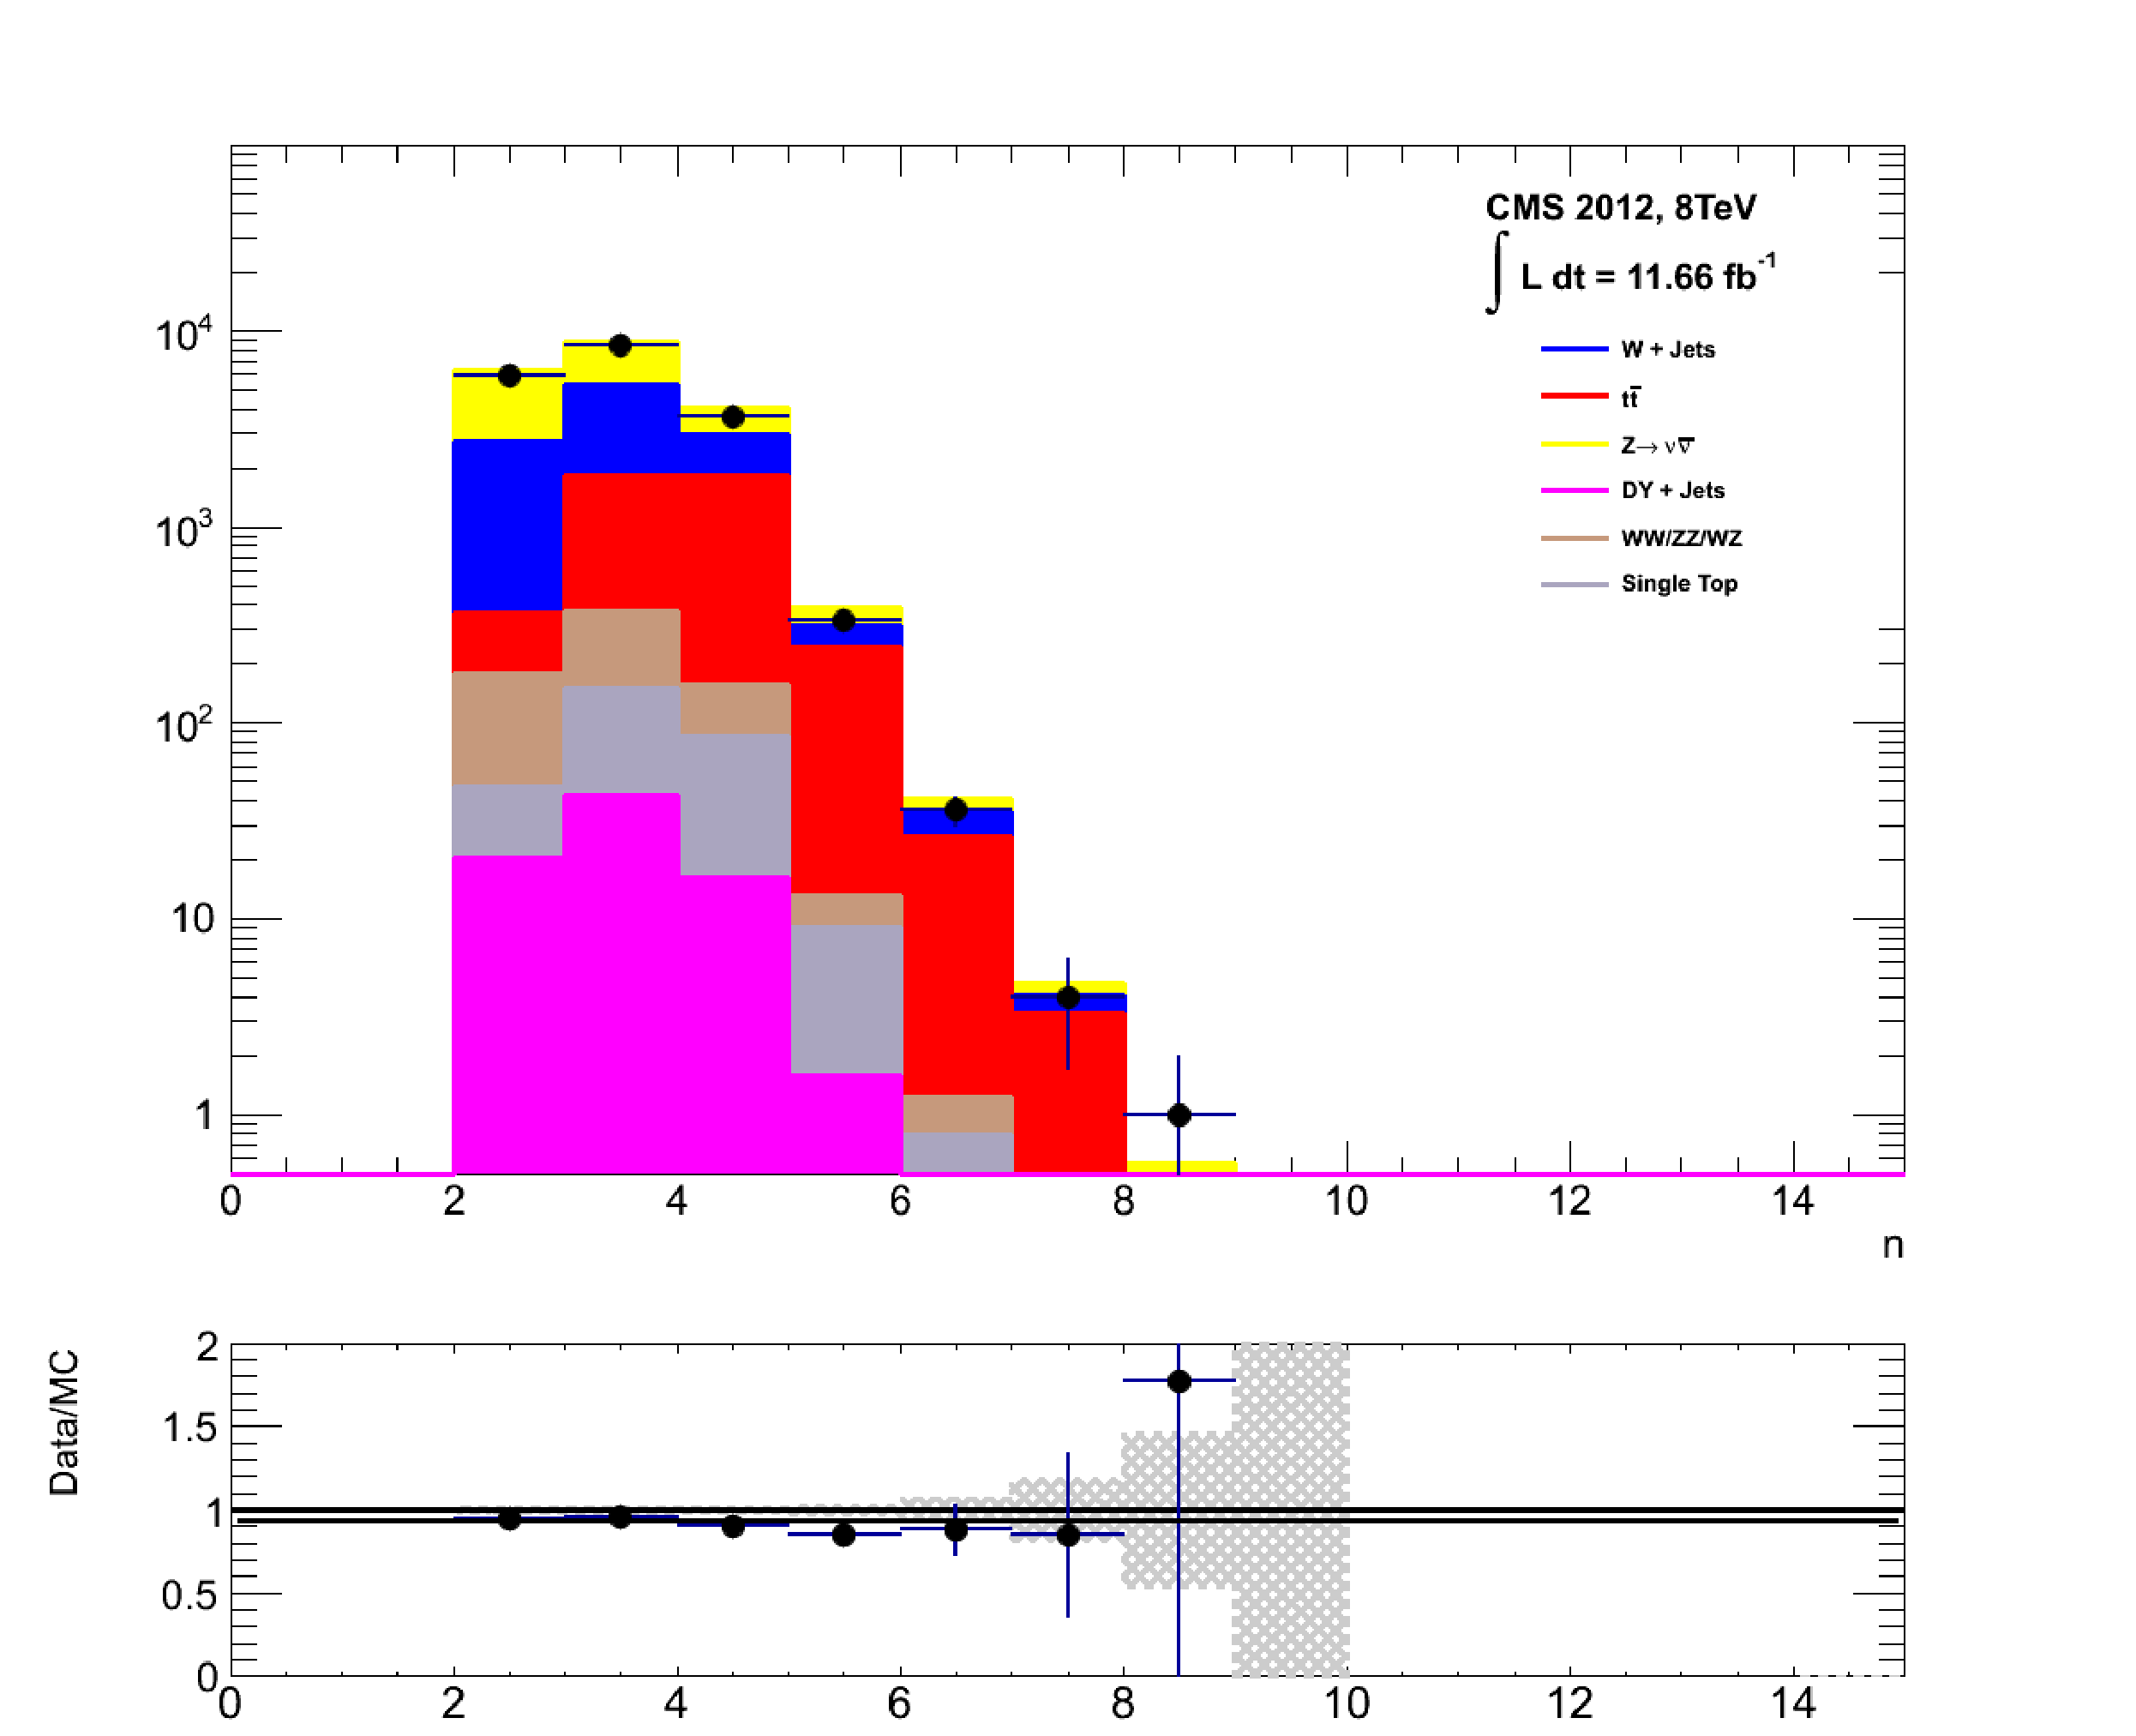
\includegraphics[width = 3.3in]{plots/had_njet_datamc.pdf}
(a) Jet Multiplicity
\end{minipage}
\begin{minipage}{.48\textwidth}
\centering
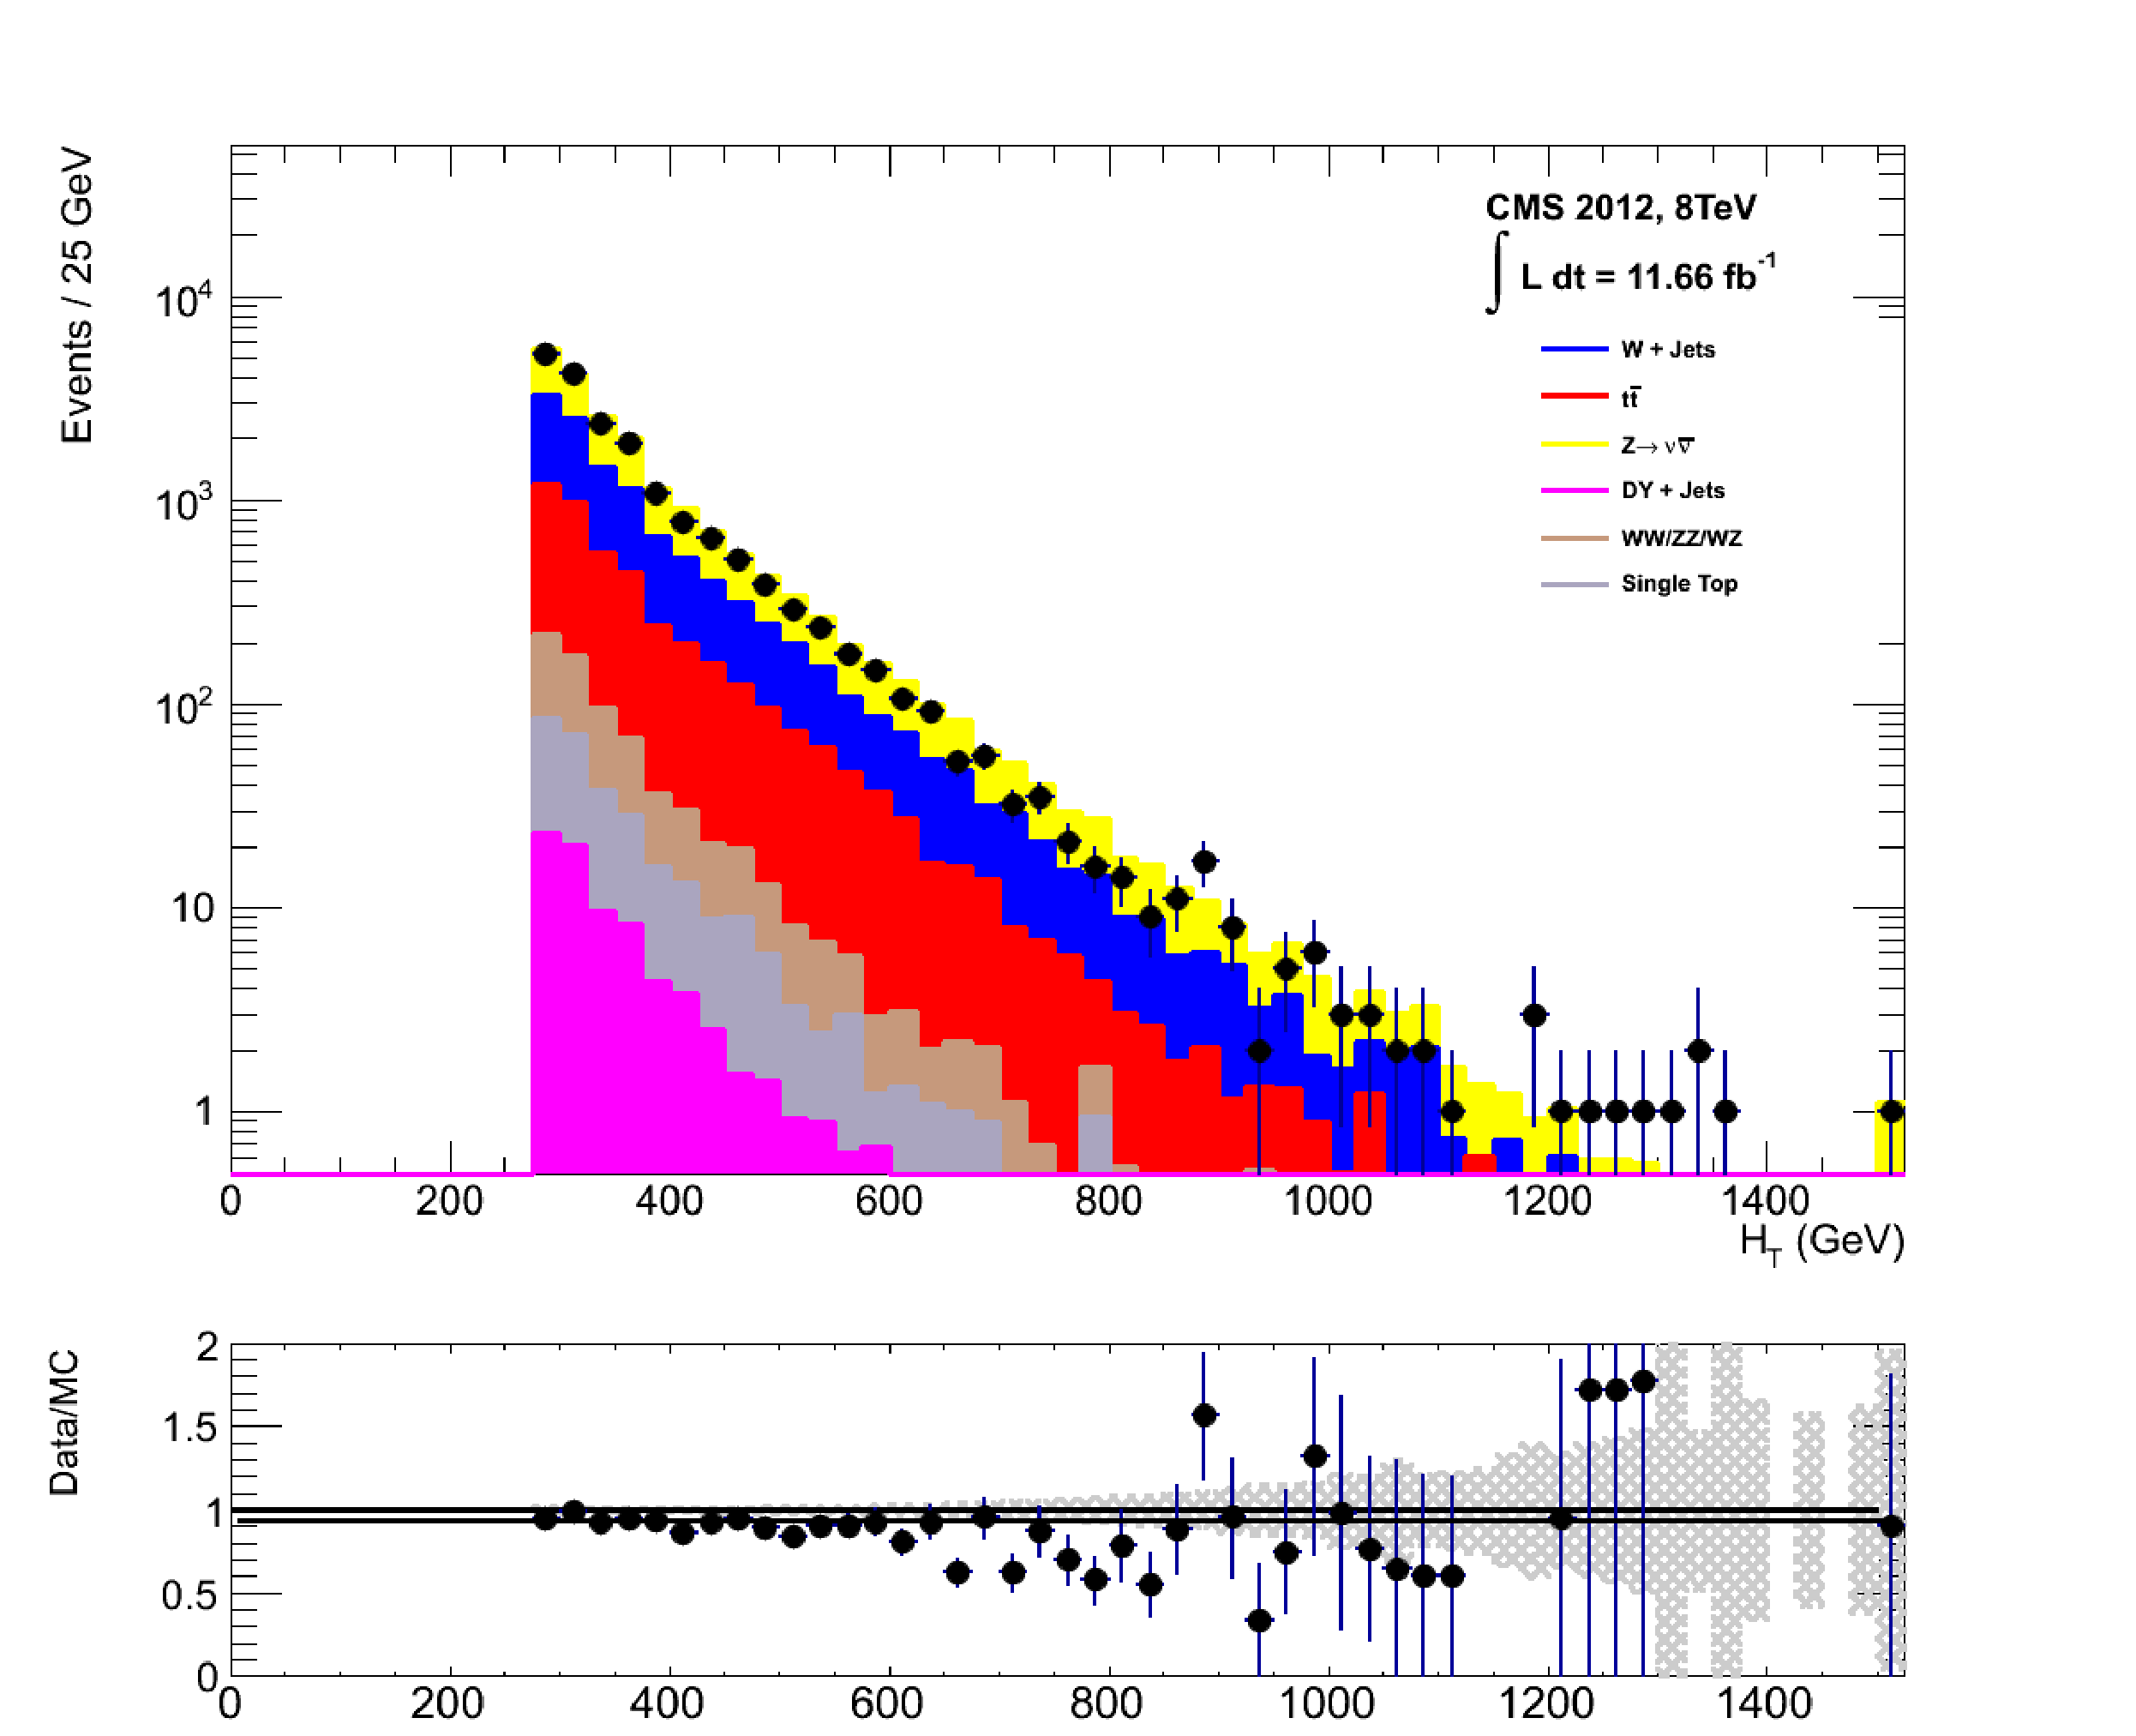
\includegraphics[width = 3.3in]{plots/had_ht_datamc.pdf}
(b) \theht
\end{minipage}
\end{minipage}

\xspace

\begin{minipage}{\linewidth}
\begin{minipage}{.48\textwidth}
\centering
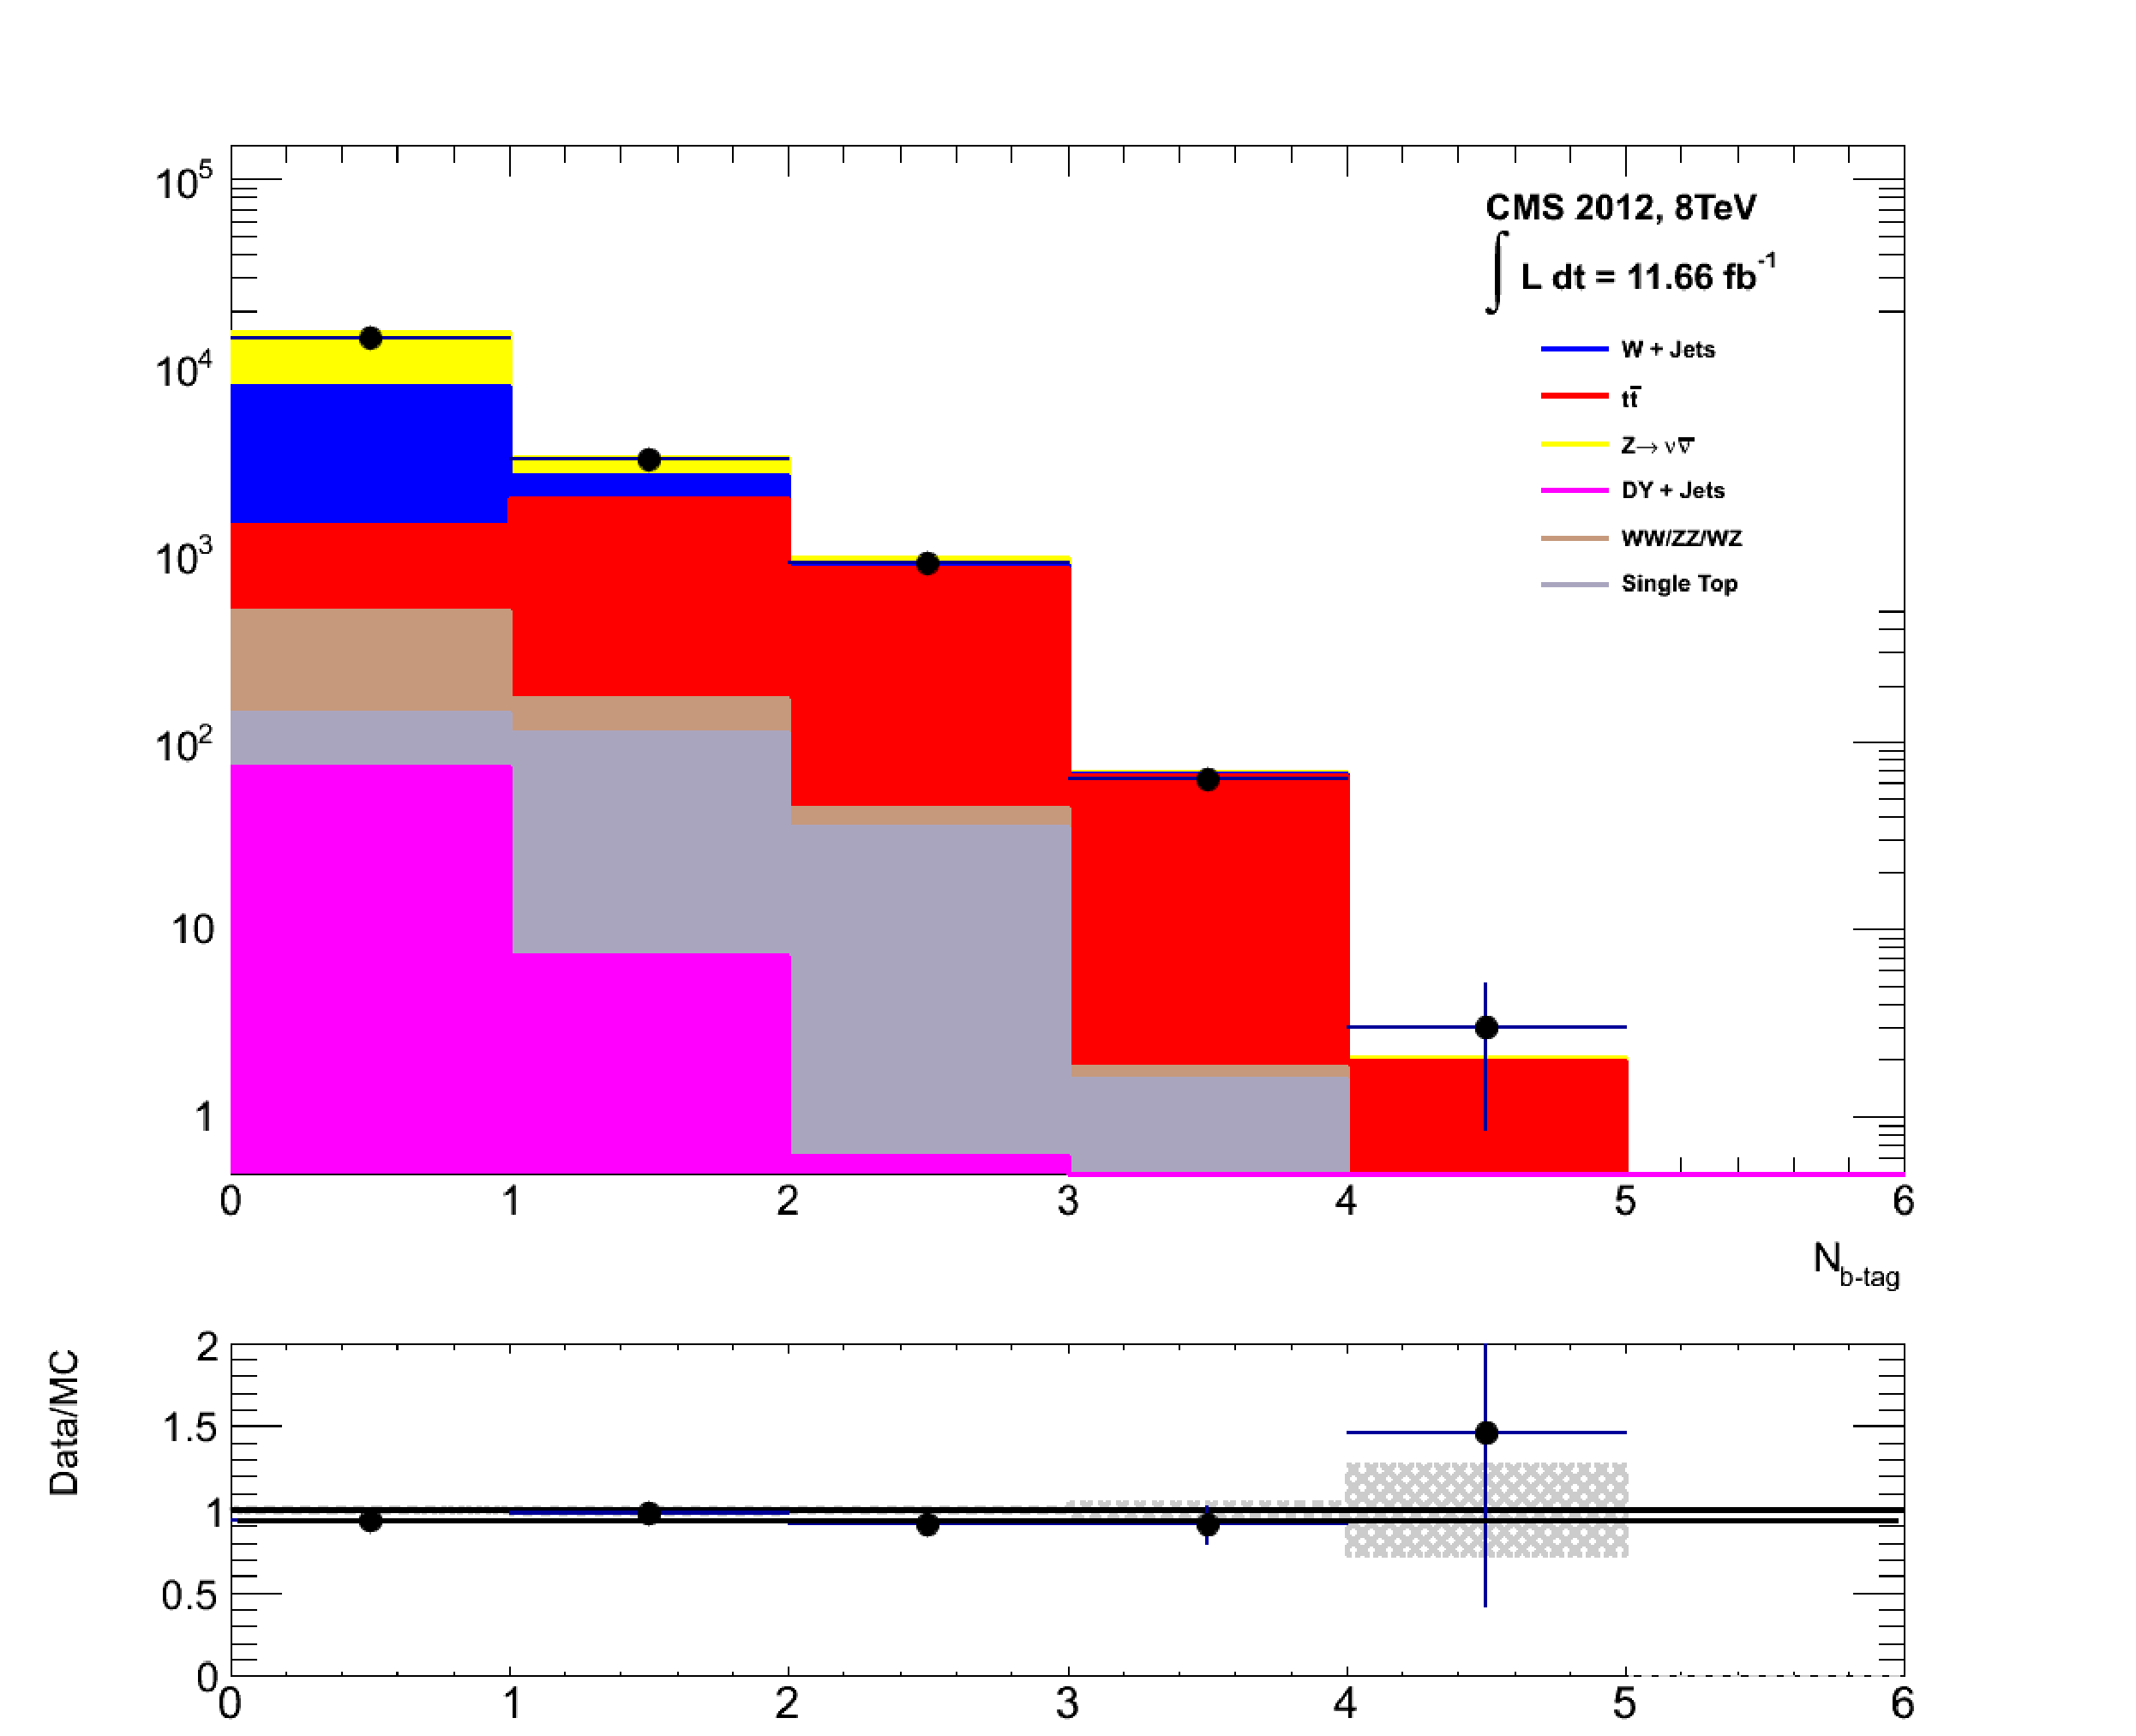
\includegraphics[width = 3.3in]{plots/had_nbtag_datamc.pdf}
$\text{(c}$) Btag Multiplicity
\end{minipage}
\begin{minipage}{.48\textwidth}
\centering
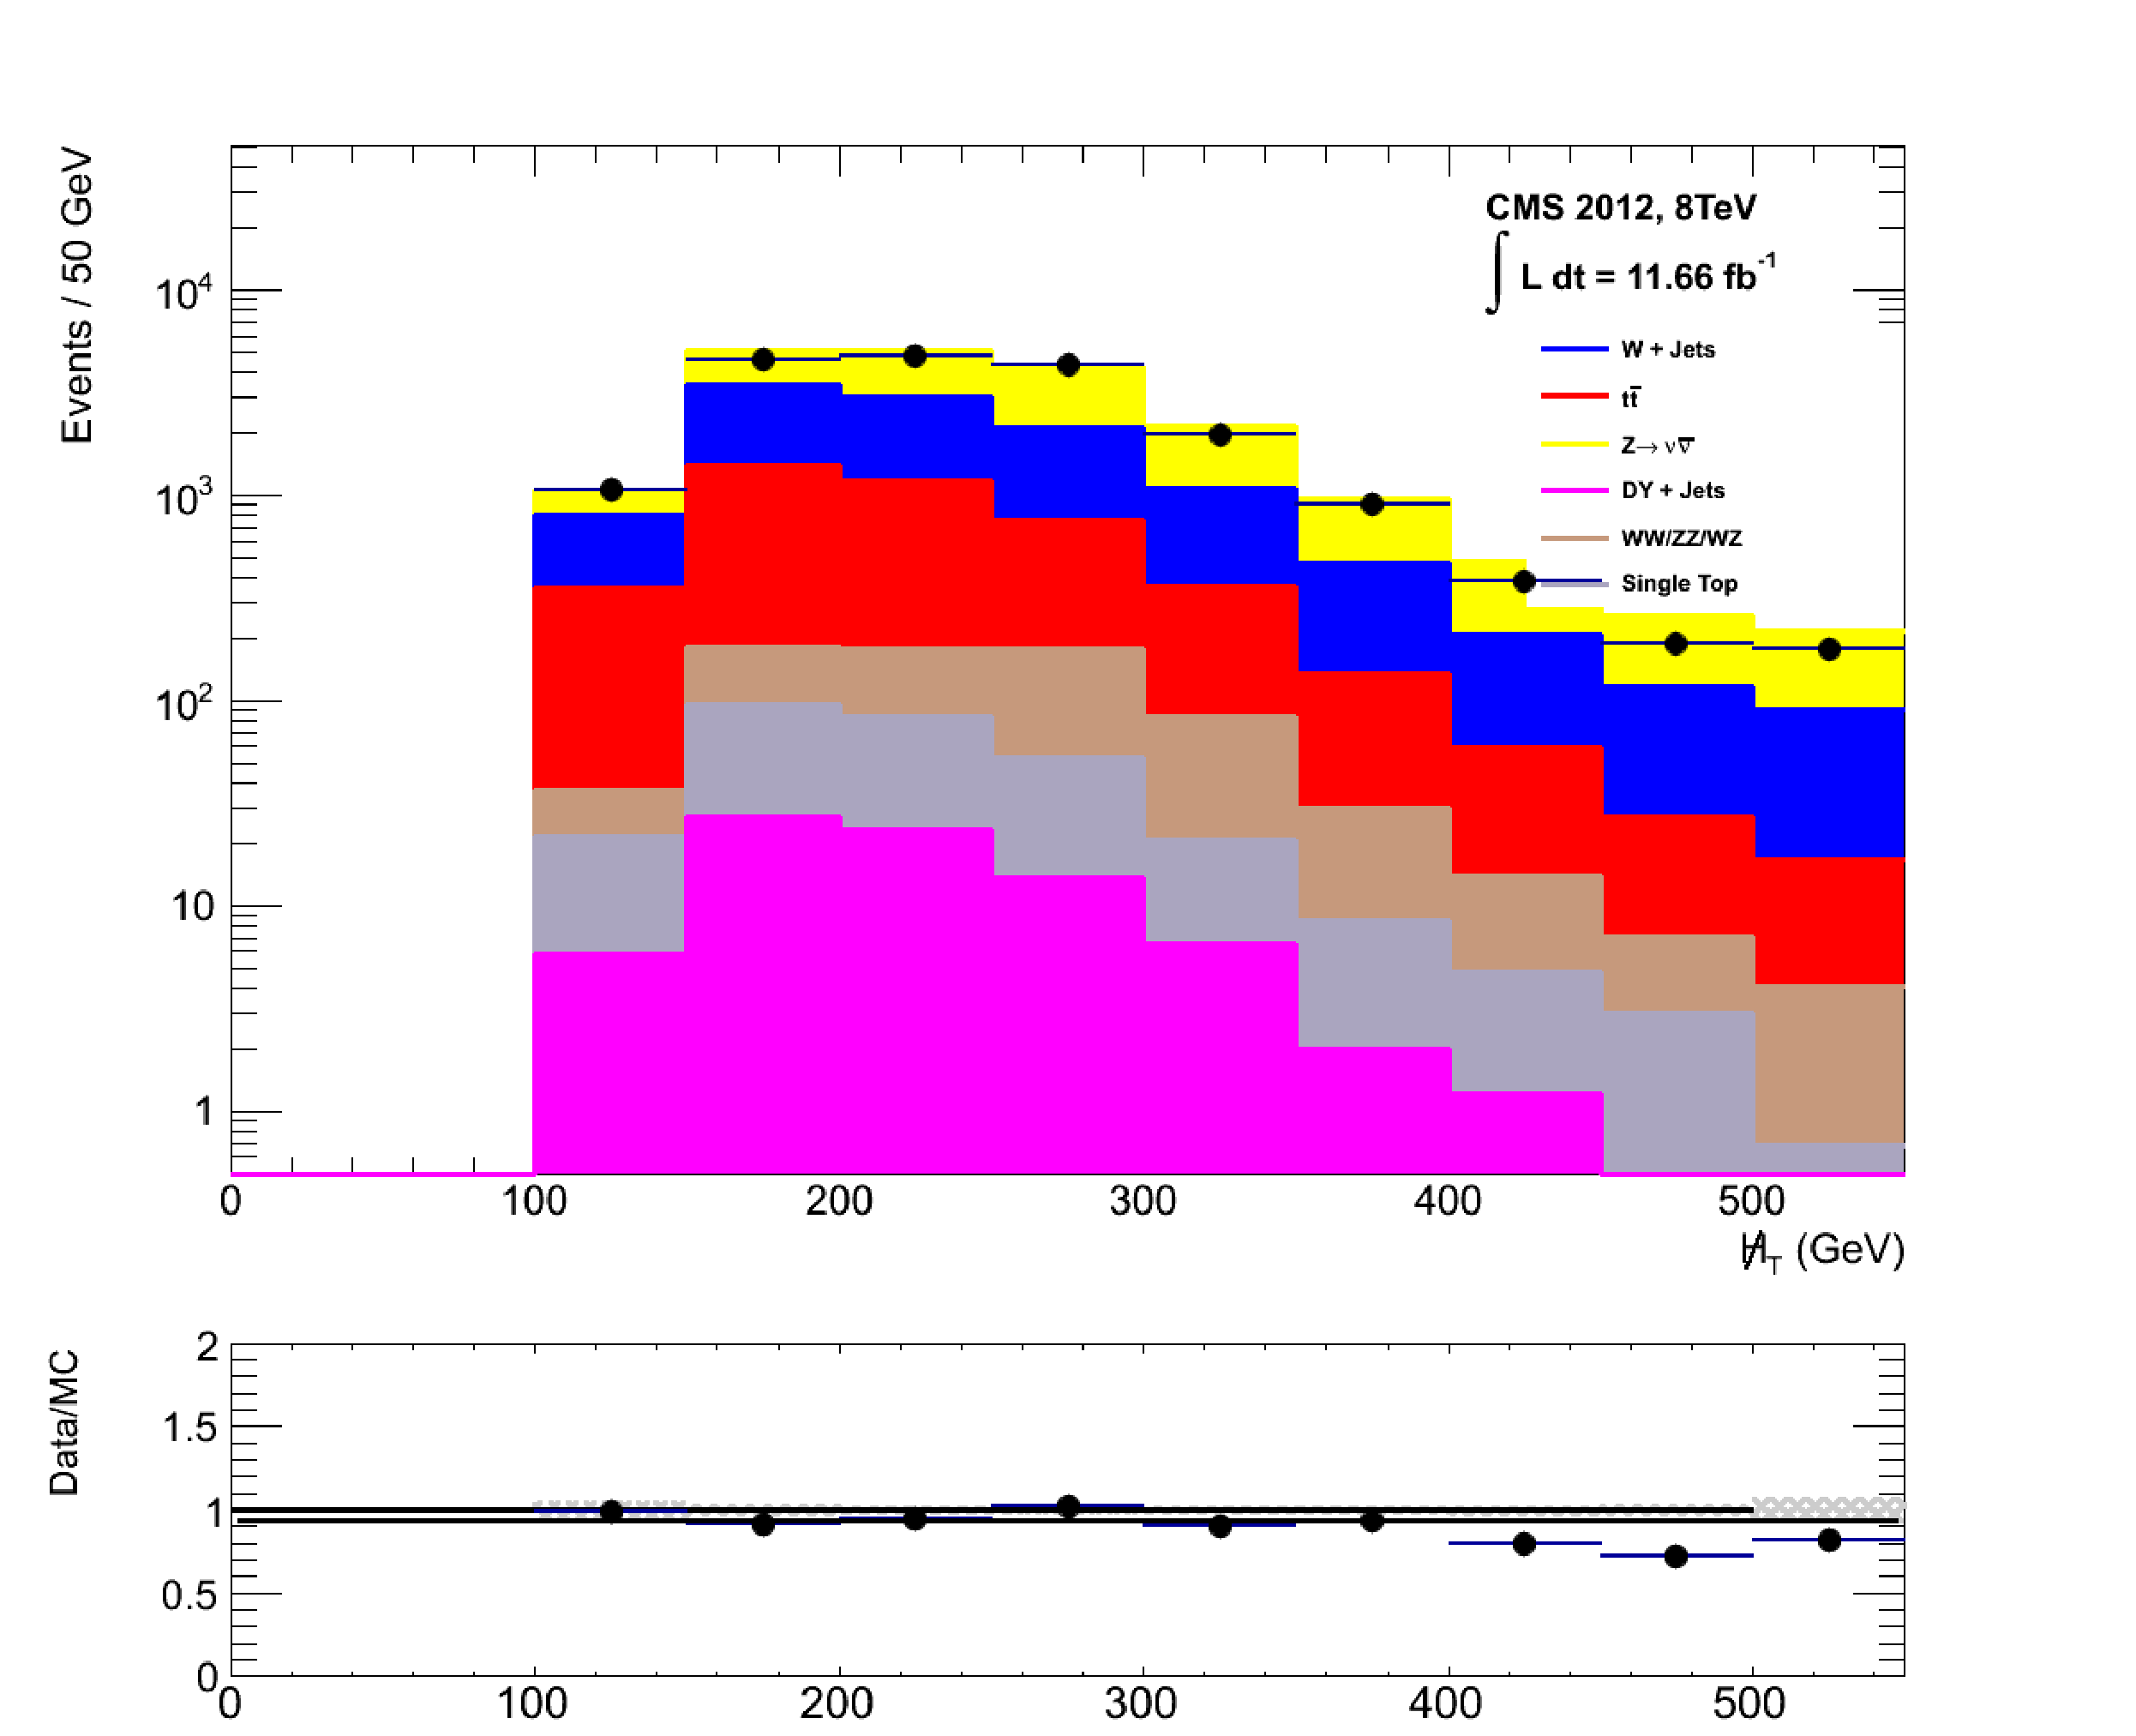
\includegraphics[width = 3.3in]{plots/had_mht_datamc.pdf}
(d) \mht
\end{minipage}
\captionof{figure}[Data/MC comparisons of key variables for the hadronic signal region.]{Data/MC comparisons of key variables for the hadronic signal region, following the application of the hadronic selection criteria and the requirements of \theht $>$ 275 \GeV and \alphat $>$ 0.55. Bands represent the uncertainties due to the statistical size of the MC samples. No requirement is made upon the number of b-tagged jets or jet multiplicity in these distributions.}\label{fig:hadmcplots}
\end{minipage}

\subsection{Control Sample Definition and Background Estimation}
\label{subsec:controlsampledefinition}

The method used to estimate the background contributions in the hadronic signal region relies on the use of a \acf{TF}. This is determined from simulation in both the control, $\text{N}_{\text{MC}}^{\text{control}}$, and signal, $\text{N}_{\text{MC}}^{\text{signal}}$, region to transform the observed yield measured in data for a control sample,  $\text{N}_{\text{obs}}^{\text{control}}$, into a background prediction, $\text{N}_{\text{pred}}^{\text{signal}}$, via Equation (\ref{eq:transfactor}),

\begin{equation}
\label{eq:transfactor}
\text{N}_{\text{pred}}^{\text{signal}} = \frac{\text{N}_{\text{MC}}^{\text{signal}}}{ \text{N}_{\text{MC}}^{\text{control}}} \times  \text{N}_{\text{obs}}^{\text{control}}.
\end{equation}

All simulation samples are normalised to the luminosity of the data samples of the relevant selection they are being applied to. Through this method, ``vanilla'' predictions for the \ac{SM} background in the signal region can be made by considering separately the sum of the prediction from the combination of either the \mupjets and \gpjets, or \mupjets and \dimupjets samples. 

It must be noted that the final background estimation from which results are interpreted, is calculated via a fitting procedure defined formally by the likelihood model described in Section (\ref{sec:statframework}). 

The sum of the expected yields from all simulated processes listed in Section (\ref{sec:alphatintroduction}), enter the denominator, $\text{N}_{\text{MC}}^{\text{control}}$, of the \ac{TF} defined in Equation (\ref{eq:transfactor}) for each control sample. However, only the specific processes being estimated by the control sample enter the numerator, $\text{N}_{\text{MC}}^{\text{signal}}$.

For the \mupjets sample the processes entering the numerator are,

\begin{equation} 
\text{N}_{\text{MC}}^{\text{signal}}(\theht,n_{\text{jet}}) = N_{W} + N_{\ttbar} + N_{DY} + N_{t} + N_{di-boson},
\end{equation}

whilst for both the \dimupjets and \gpjets samples the only simulated processes used in the numerator is,

\begin{equation} 
\text{N}_{\text{MC}}^{\text{signal}}(\theht,n_{\text{jet}}) = N_{\zinv}.
\end{equation}

The control samples and the \ac{EWK} processes they are specifically tuned to select are defined below, with distributions of key variables for each of the control samples shown for illustrative purposes in Figures \ref{fig:muonmcplots}, \ref{fig:dimuonmcplots} and \ref{fig:photonmcplots}. No requirement is placed upon the number of b-tagged jets or jet multiplicity in the distributions shown. The distributions highlight the background compositions of each control sample, where in general, good agreement is observed between data and simulation, giving confidence that the samples are well understood. The contribution from QCD multi-jet events is expected to be negligible: 

\begin{itemize} 

\item[] \textbf{The \mupjets control sample}

Events from W + jets and \ttbar processes enter into the hadronic signal sample due to unidentified leptons from acceptance effects or reconstruction inefficiencies and hadronic tau decays. These leptons originate from the decay of high \pt W bosons. 

The control sample specifically identify $W \rightarrow \mu\bar{\nu}$ decays within a similar phase-space of the signal region, where the muon is subsequently ignored in the calculation of event level variables, i.e. \theht, \mht, \alphat. 

All kinematic jet-based selection criteria are identical to those applied in the hadronic search region (with the exception of an \alphat, requirement discussed below) detailed in Section (\ref{subsec:eventselection}), with the same \theht, jet multiplicity and b-jet multiplicity categorisation described previously. Furthermore, the following selection criteria are also required:

\begin{itemize}
\item Muons originating from W boson decays are selected by requiring one tightly isolated muon defined in Table \ref{tab:muonidtable}, with a \pt $>$ 30 \GeV and \abeta $<$ 2.1. Both of these thresholds arise from trigger restrictions.  
\item The transverse mass of the W candidate must satisfy \mt$(\mu,\met) >$ 30 \GeV ( to suppress QCD multi-jet events). 
\item Events which contain a jet overlapping with a muon $\Delta \text{R}(\mu,\text{jet}) <$ 0.5 are vetoed to remove events from muons produced as part of a jet's hadronisation process. 
\item Events containing a second muon candidate which has failed id, but passing \pt and \abeta requirements, are checked to have an invariant mass that satisfies $ \lvert M_{\mu\mu} - m_{Z}\rvert >$ 25, thus removing $Z \rightarrow \mu\mu$ contamination.
\end{itemize}


\begin{minipage}{\linewidth}
\centering
\begin{minipage}{.48\textwidth}
\centering
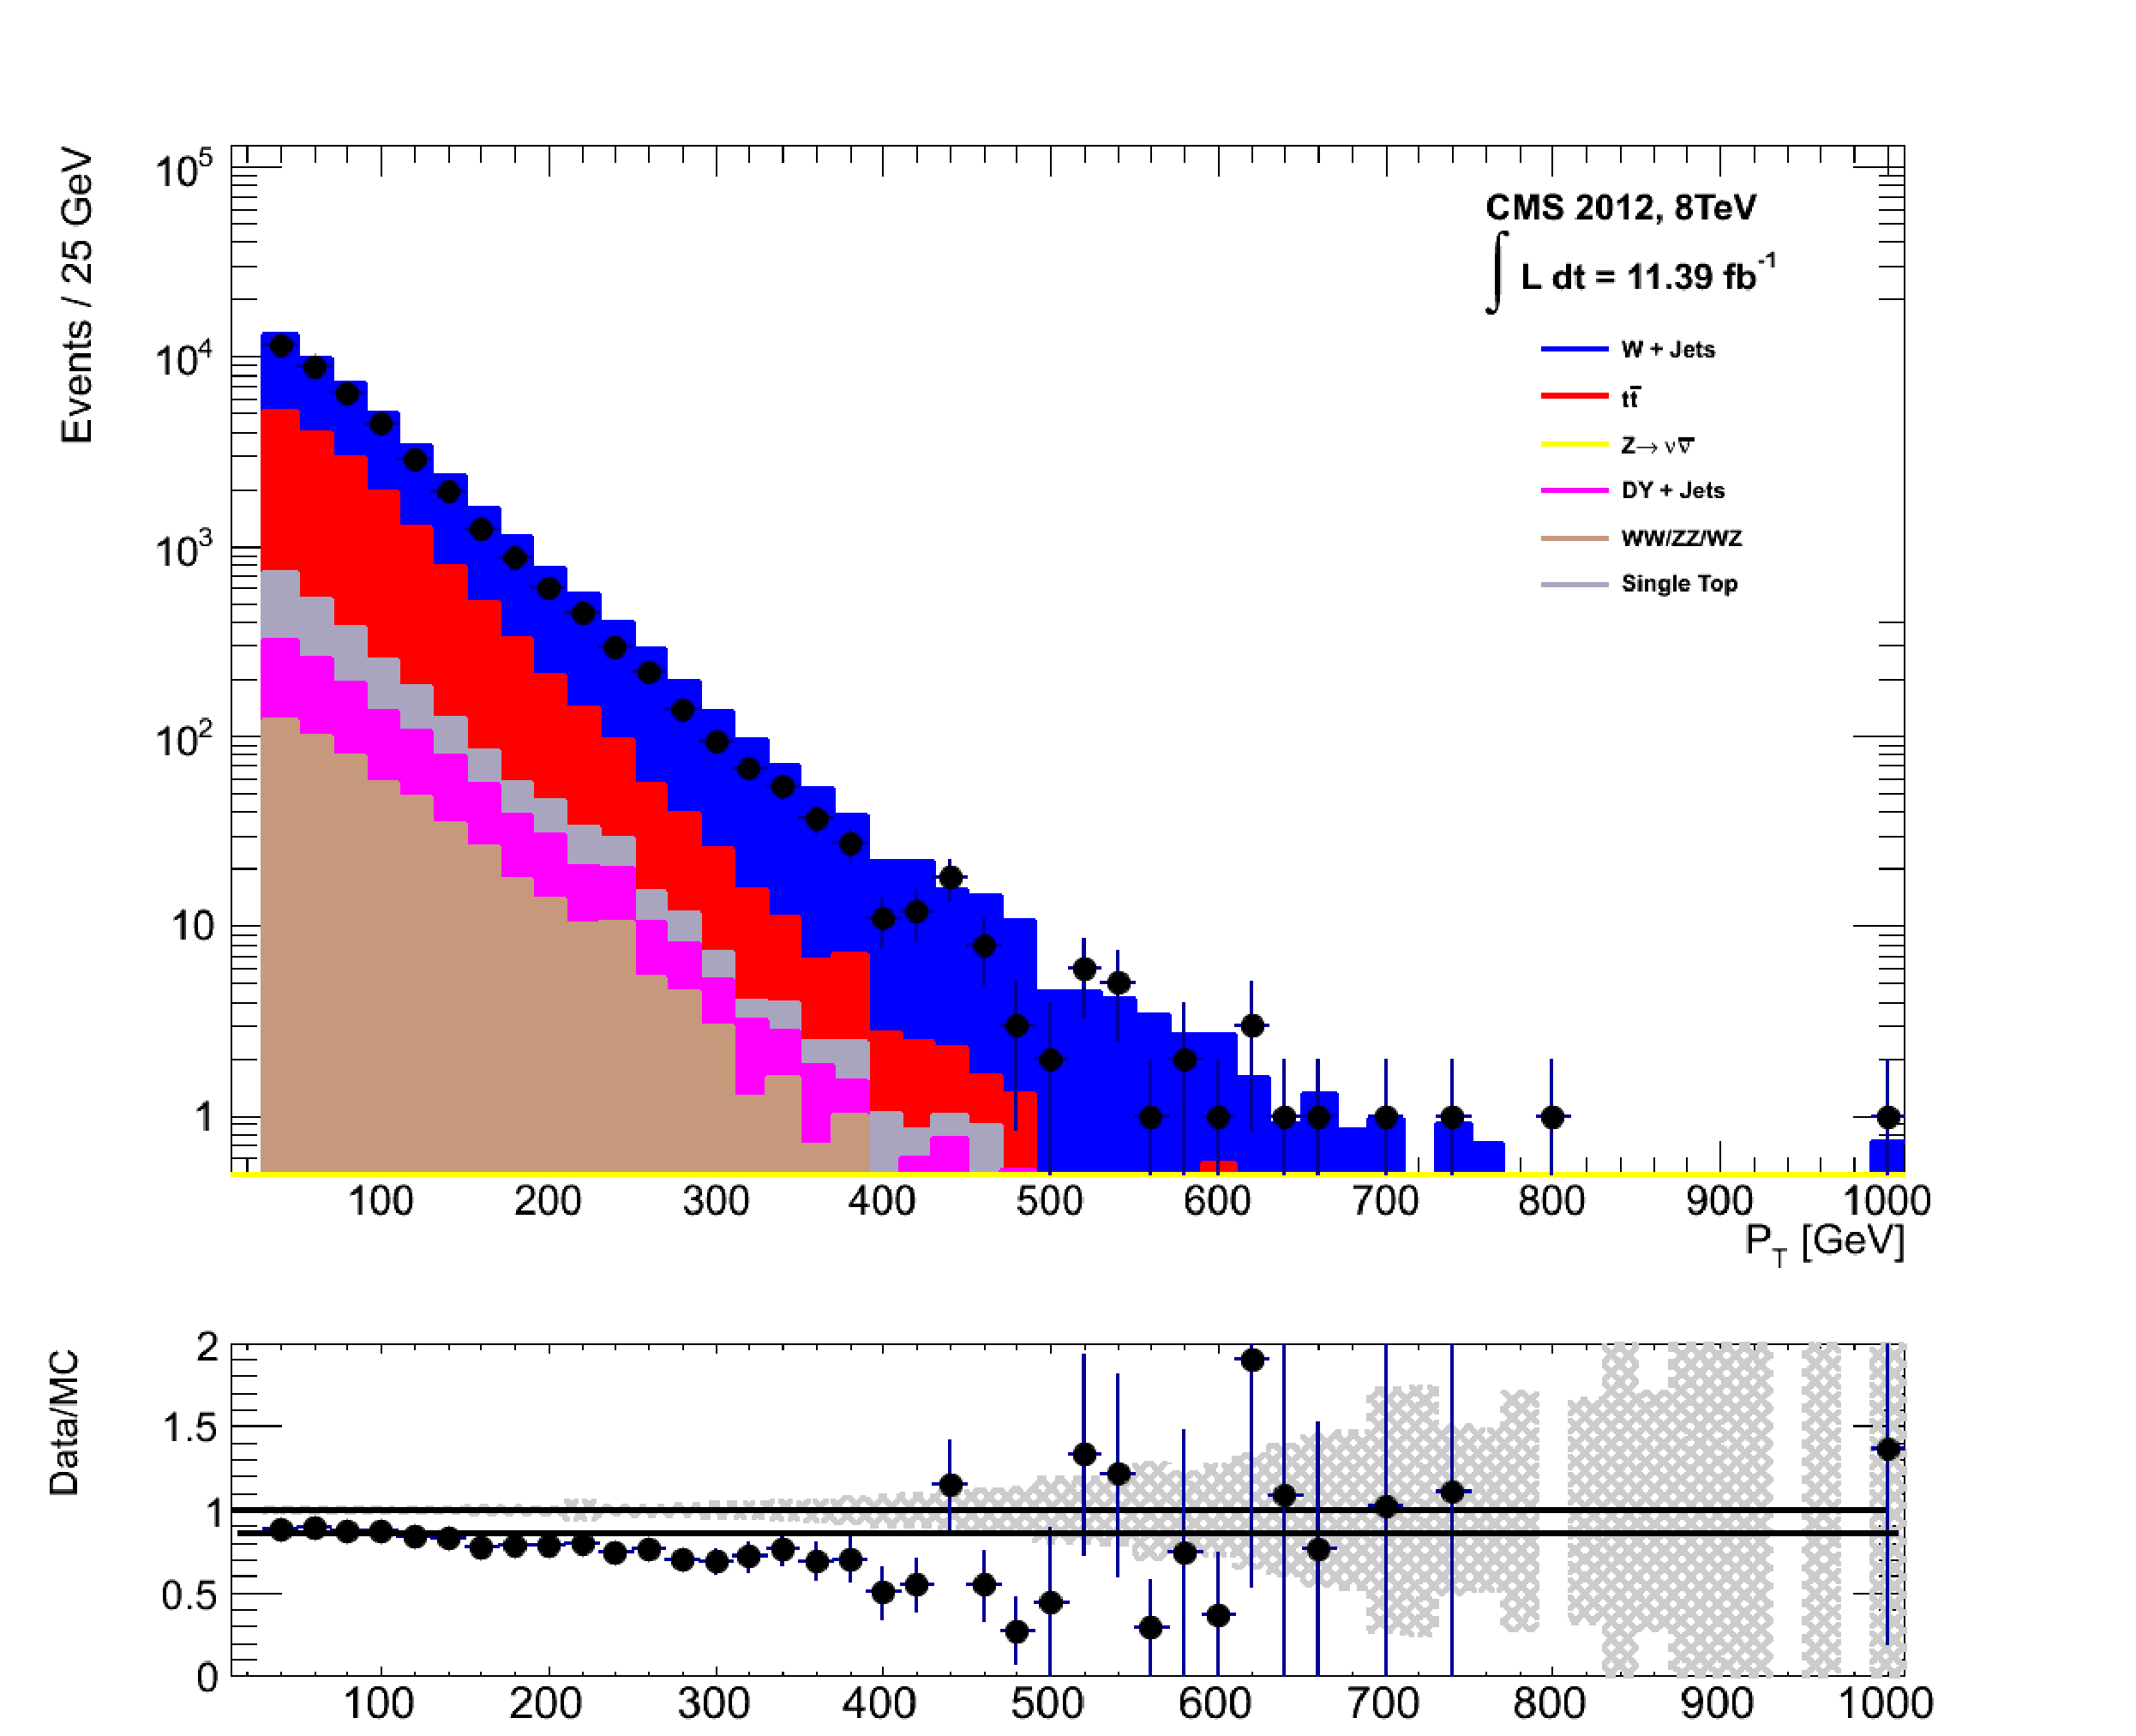
\includegraphics[width = 3.2in]{plots/muon_leadmu_datamc.pdf}
(a) Lead Muon \pt
\end{minipage}
\begin{minipage}{.48\textwidth}
\centering
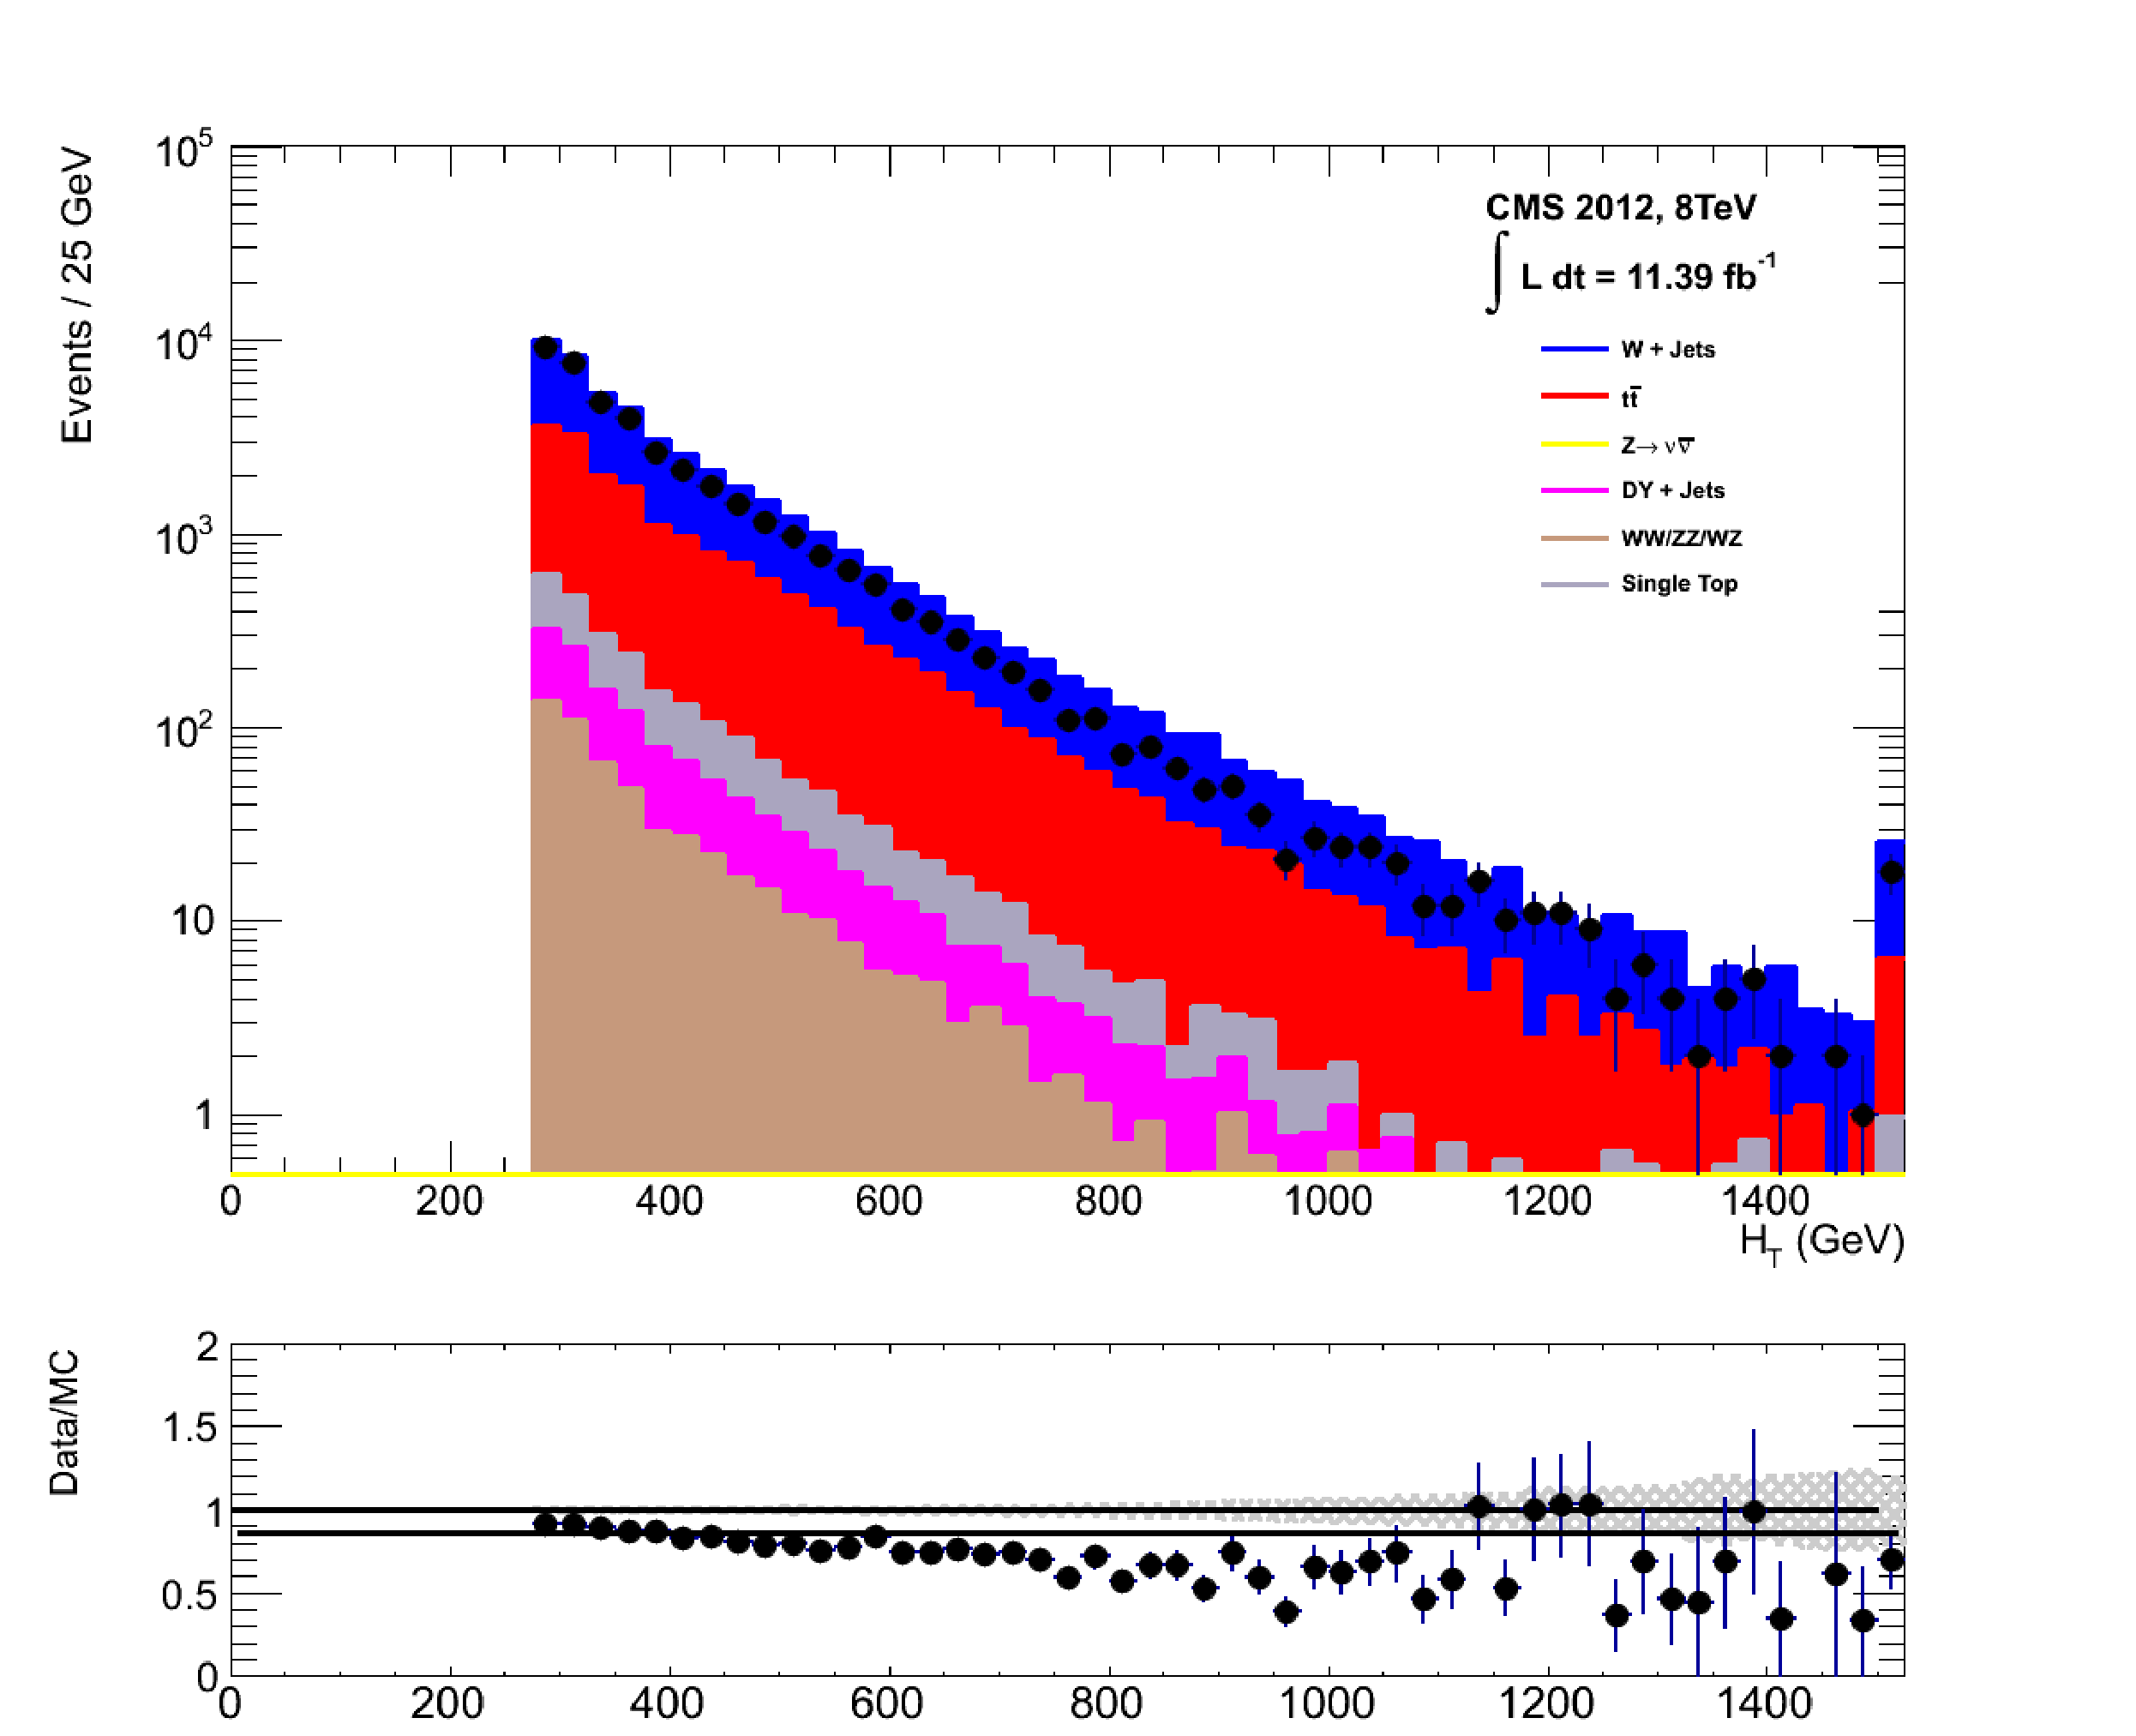
\includegraphics[width = 3.2in]{plots/muon_ht_datamc.pdf}
(b) \theht
\end{minipage}
\end{minipage}

\xspace

\begin{minipage}{\linewidth}
\centering
\begin{minipage}{.48\textwidth}
\centering
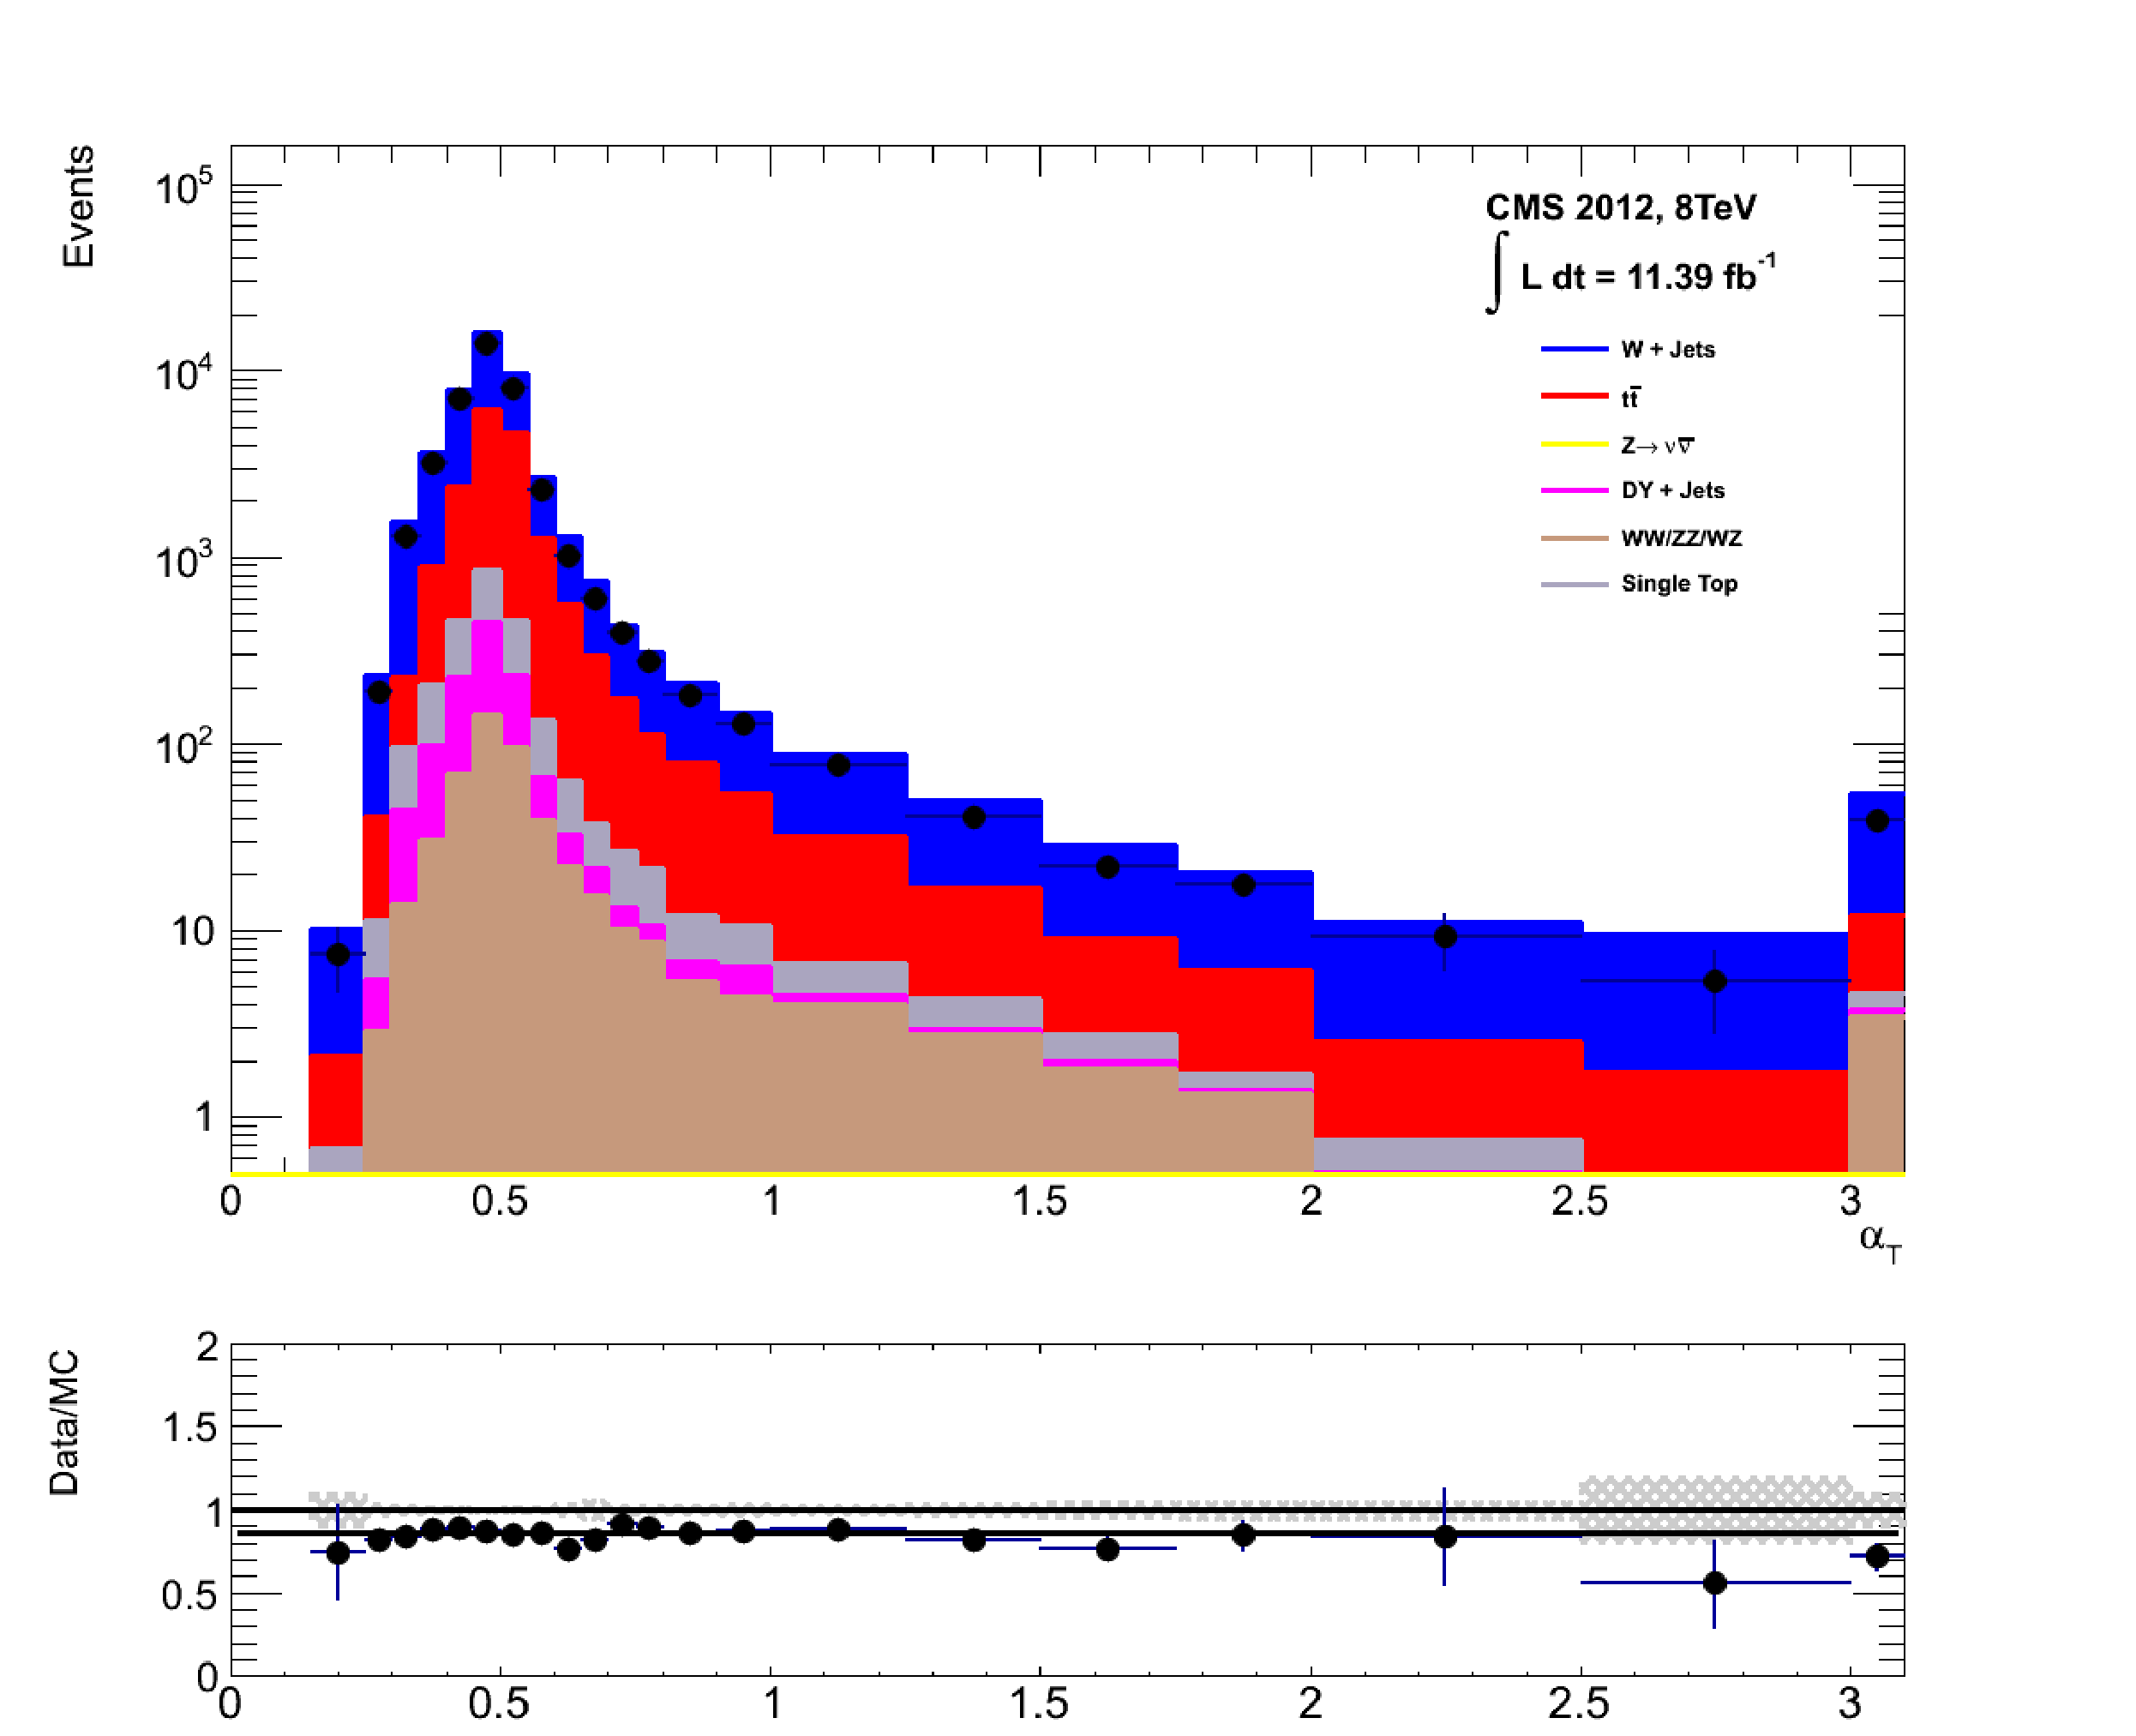
\includegraphics[width = 3.2in]{plots/muon_alphat_datamc.pdf}
$\text{(c}$) \alphat
\end{minipage}
\begin{minipage}{.48\textwidth}
\centering
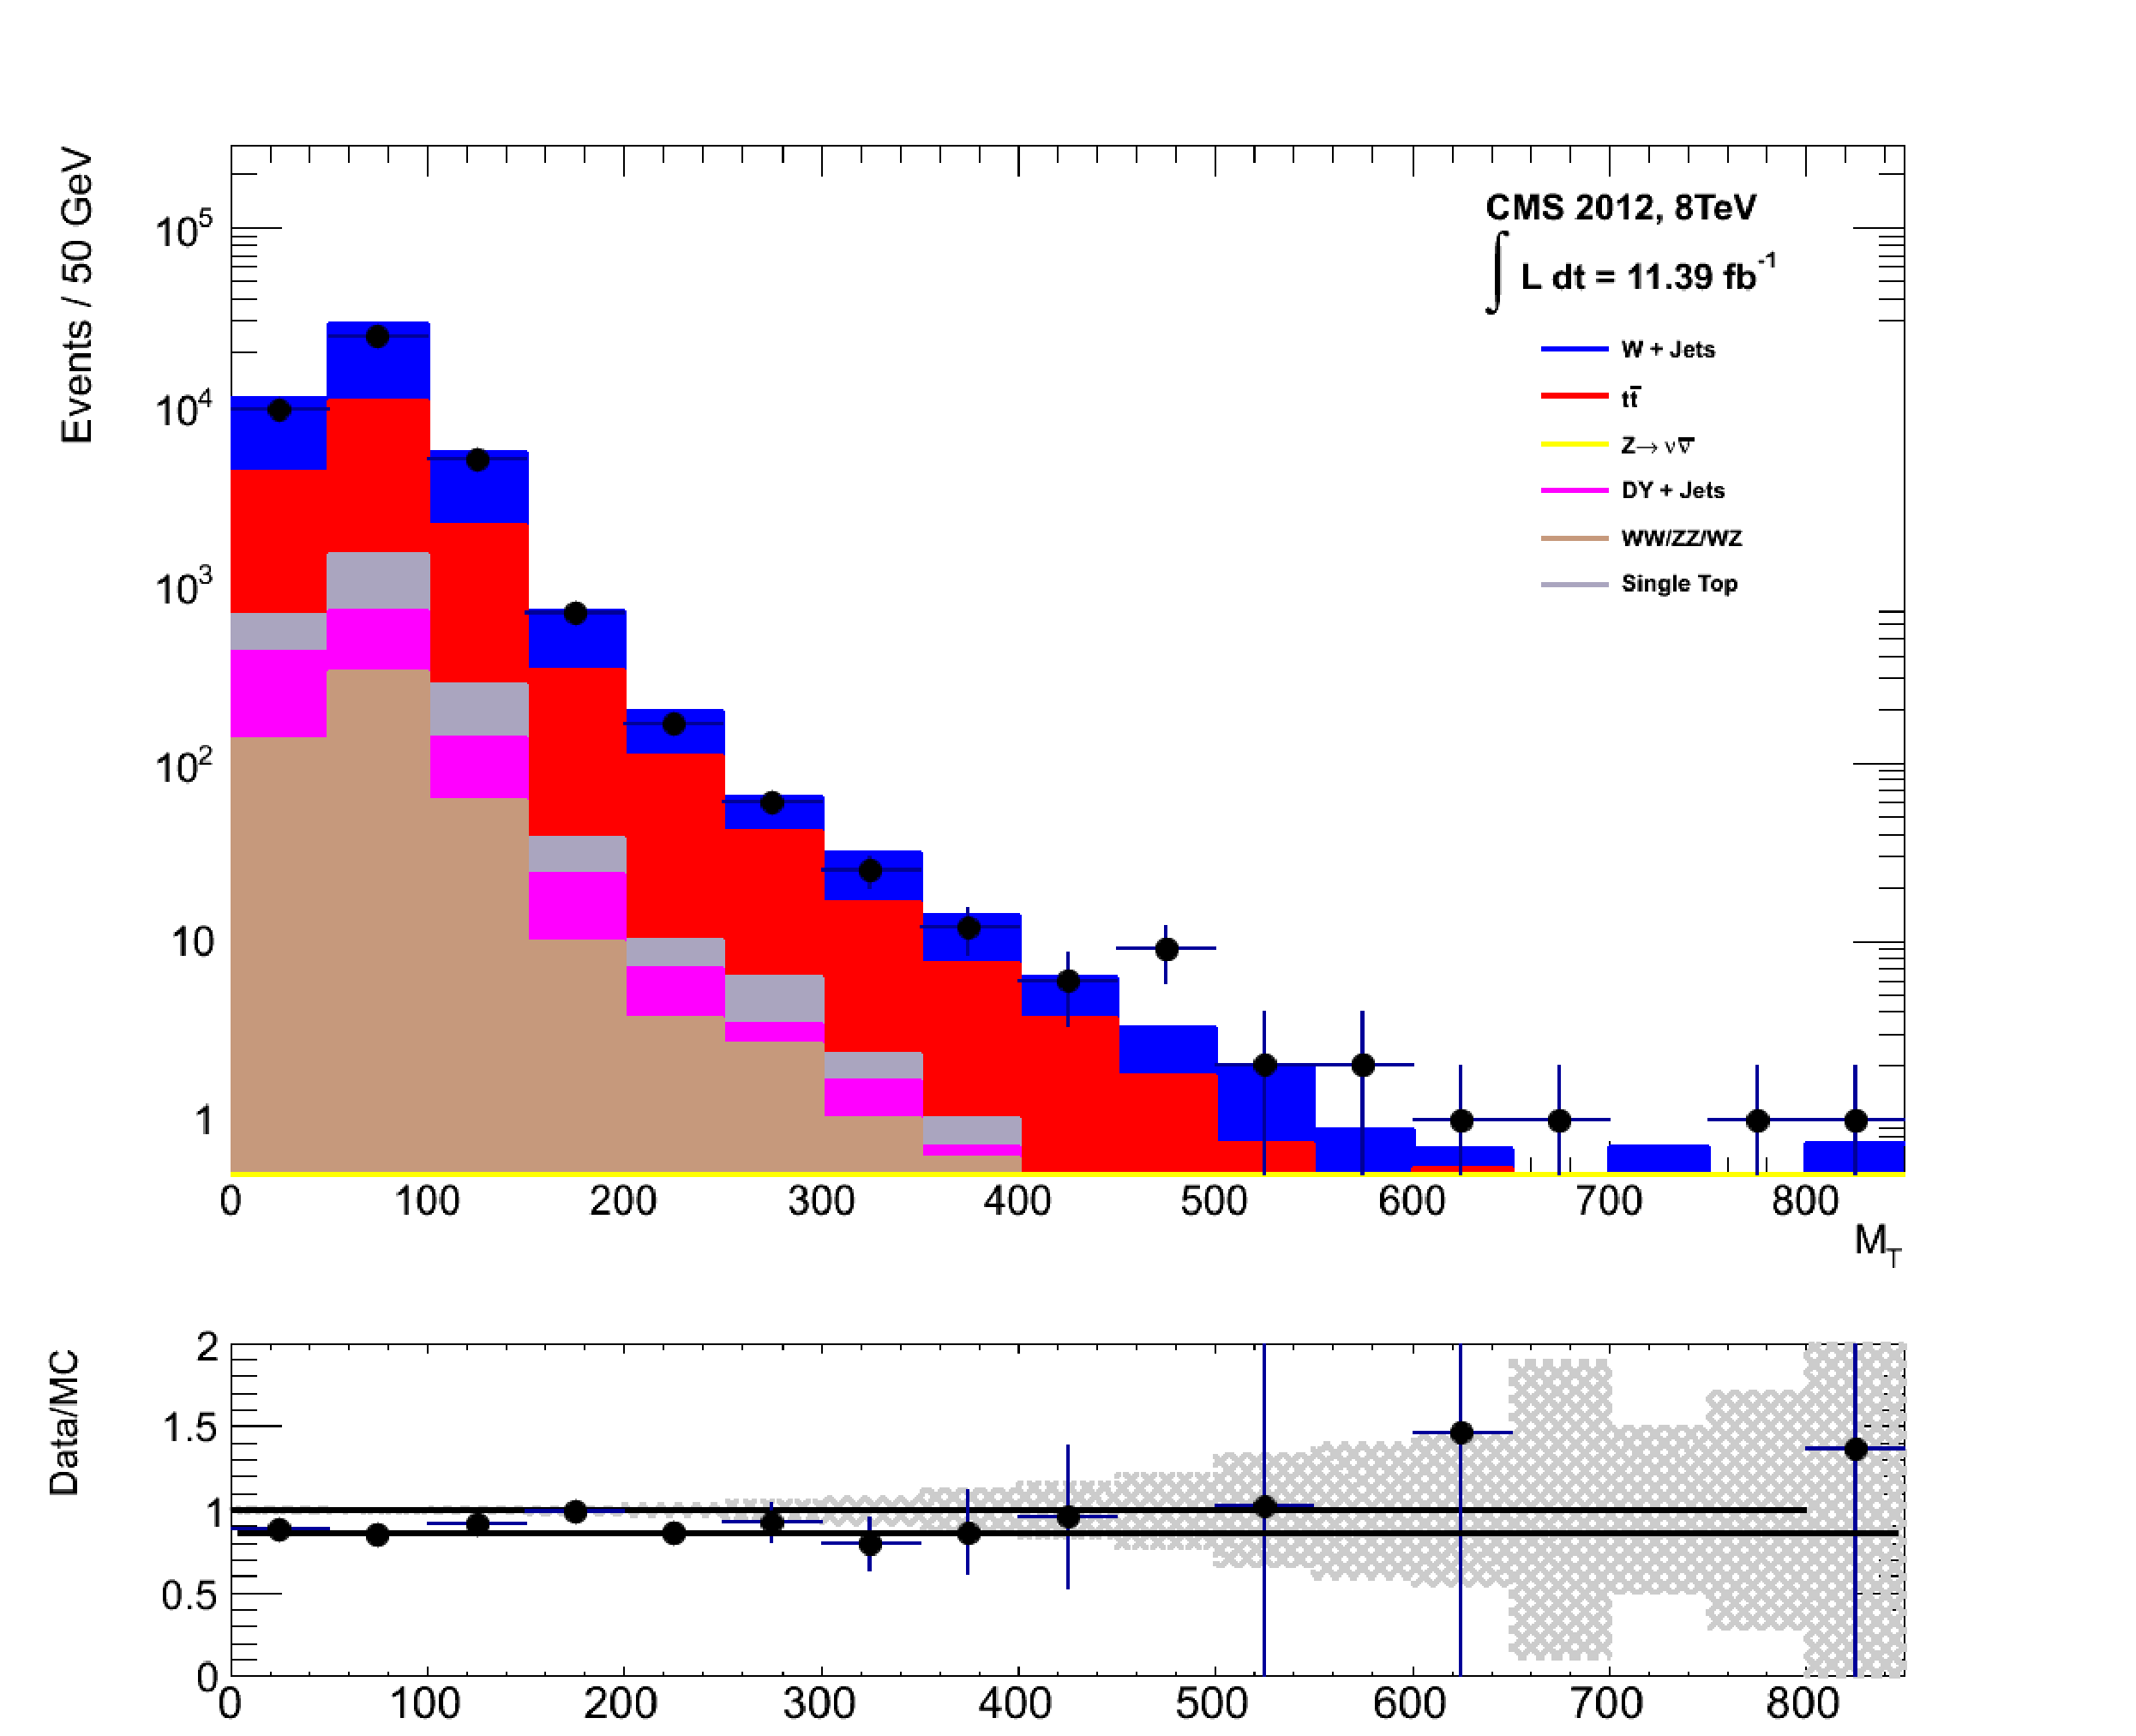
\includegraphics[width = 3.2in]{plots/muon_mt_datamc.pdf}
(d) Transverse mass $M_{T}$
\end{minipage}
\captionof{figure}[Data/MC comparisons of key variables for the \mupjets selection.]{Data/MC comparisons of key variables for the \mupjets selection,following the application of selection criteria and the requirements that \theht $>$ 275 \GeV. Bands represent the uncertainties due to the statistical size of the MC samples. No requirement is made upon the number of b-tagged jets or jet multiplicity in these distributions.}\label{fig:muonmcplots}
\end{minipage}

\item[] \textbf{The \dimupjets control sample}

An irreducible \zinv + jets background enters into the signal region from genuine \met from the escaping neutrinos. This background is estimated using two control samples, the first of which is the \zmumu + jets process, which posses identical kinematic properties, but with a different acceptance and branching ratio \cite{pdg2012}.

The same acceptance requirements as the \mupjets selection for muons is applied, as defined in Table  \ref{tab:muonidtable}. Muons in the event are ignored for the purpose of the calculation of event level variables. In addition to kinematic jet-based selection criteria (with the exception of an \alphat requirement, discussed below) and event categorisation, which are identical to the hadronic search region, the following selection criteria are also specified:

\begin{itemize}
\item Muons originating from a Z boson decay are selected, requiring exactly two tightly isolated muons. Due to trigger requirements the leading muon is required to have  \pt $>$ 30 \GeV and \abeta $<$ 2.1. The requirement of the \pt on the second muon is relaxed to 10 \GeV.
\item Events are vetoed if containing a jet overlapping with a muon $\Delta \text{R}(\mu,\text{jet}) <$ 0.5. 
\item In order to specifically select two muons both originating from a single Z boson decay, the invariant mass of the two muons must satisfy $ \lvert M_{\mu\mu} - m_{Z}\rvert <$ 25. 
\end{itemize}

The \dimupjets sample is able to make predictions in the signal region of the two lowest \theht bins, providing coverage where the \gpjets sample is unable to, due to trigger requirements. In higher \theht bins, the higher event statistics of the \gpjets sample is also used in determining the \zinv estimation.

\begin{minipage}{\linewidth}
\centering
\begin{minipage}{.48\textwidth}
\centering
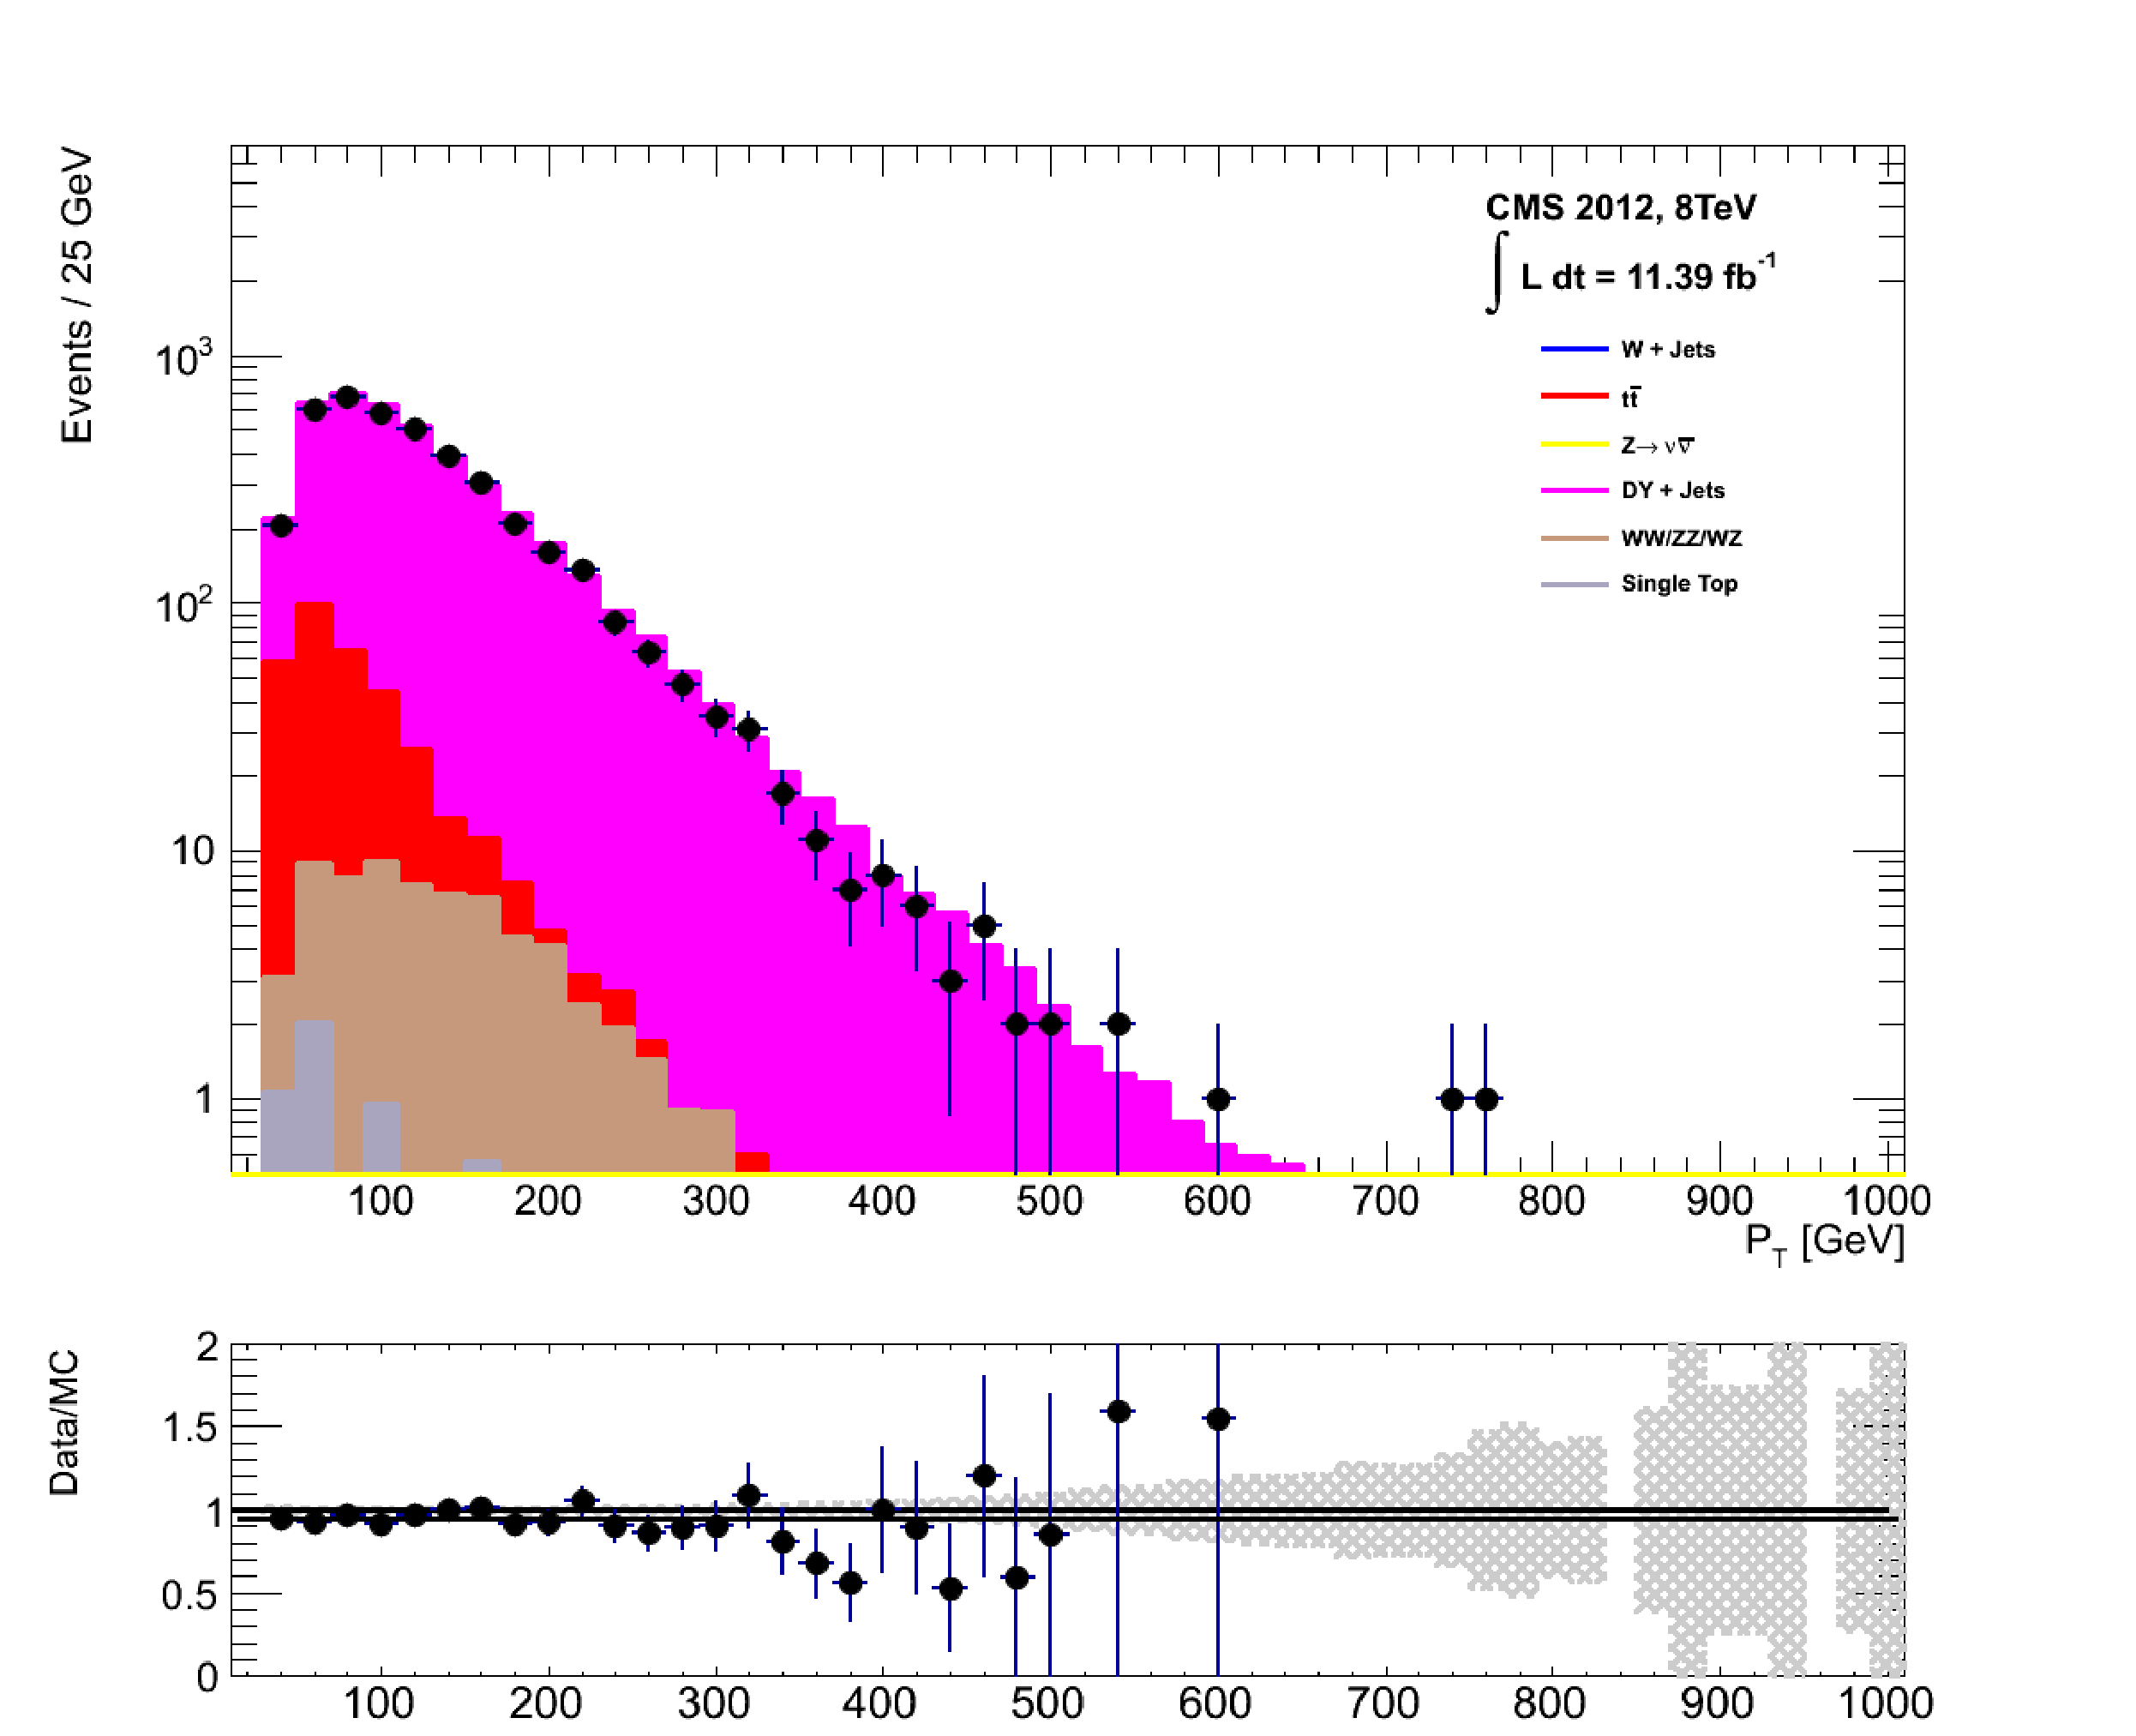
\includegraphics[width = 3.2in]{plots/dimuon_leadmu_datamc.pdf}
(a) Lead Muon \pt
\end{minipage}
\begin{minipage}{.48\textwidth}
\centering
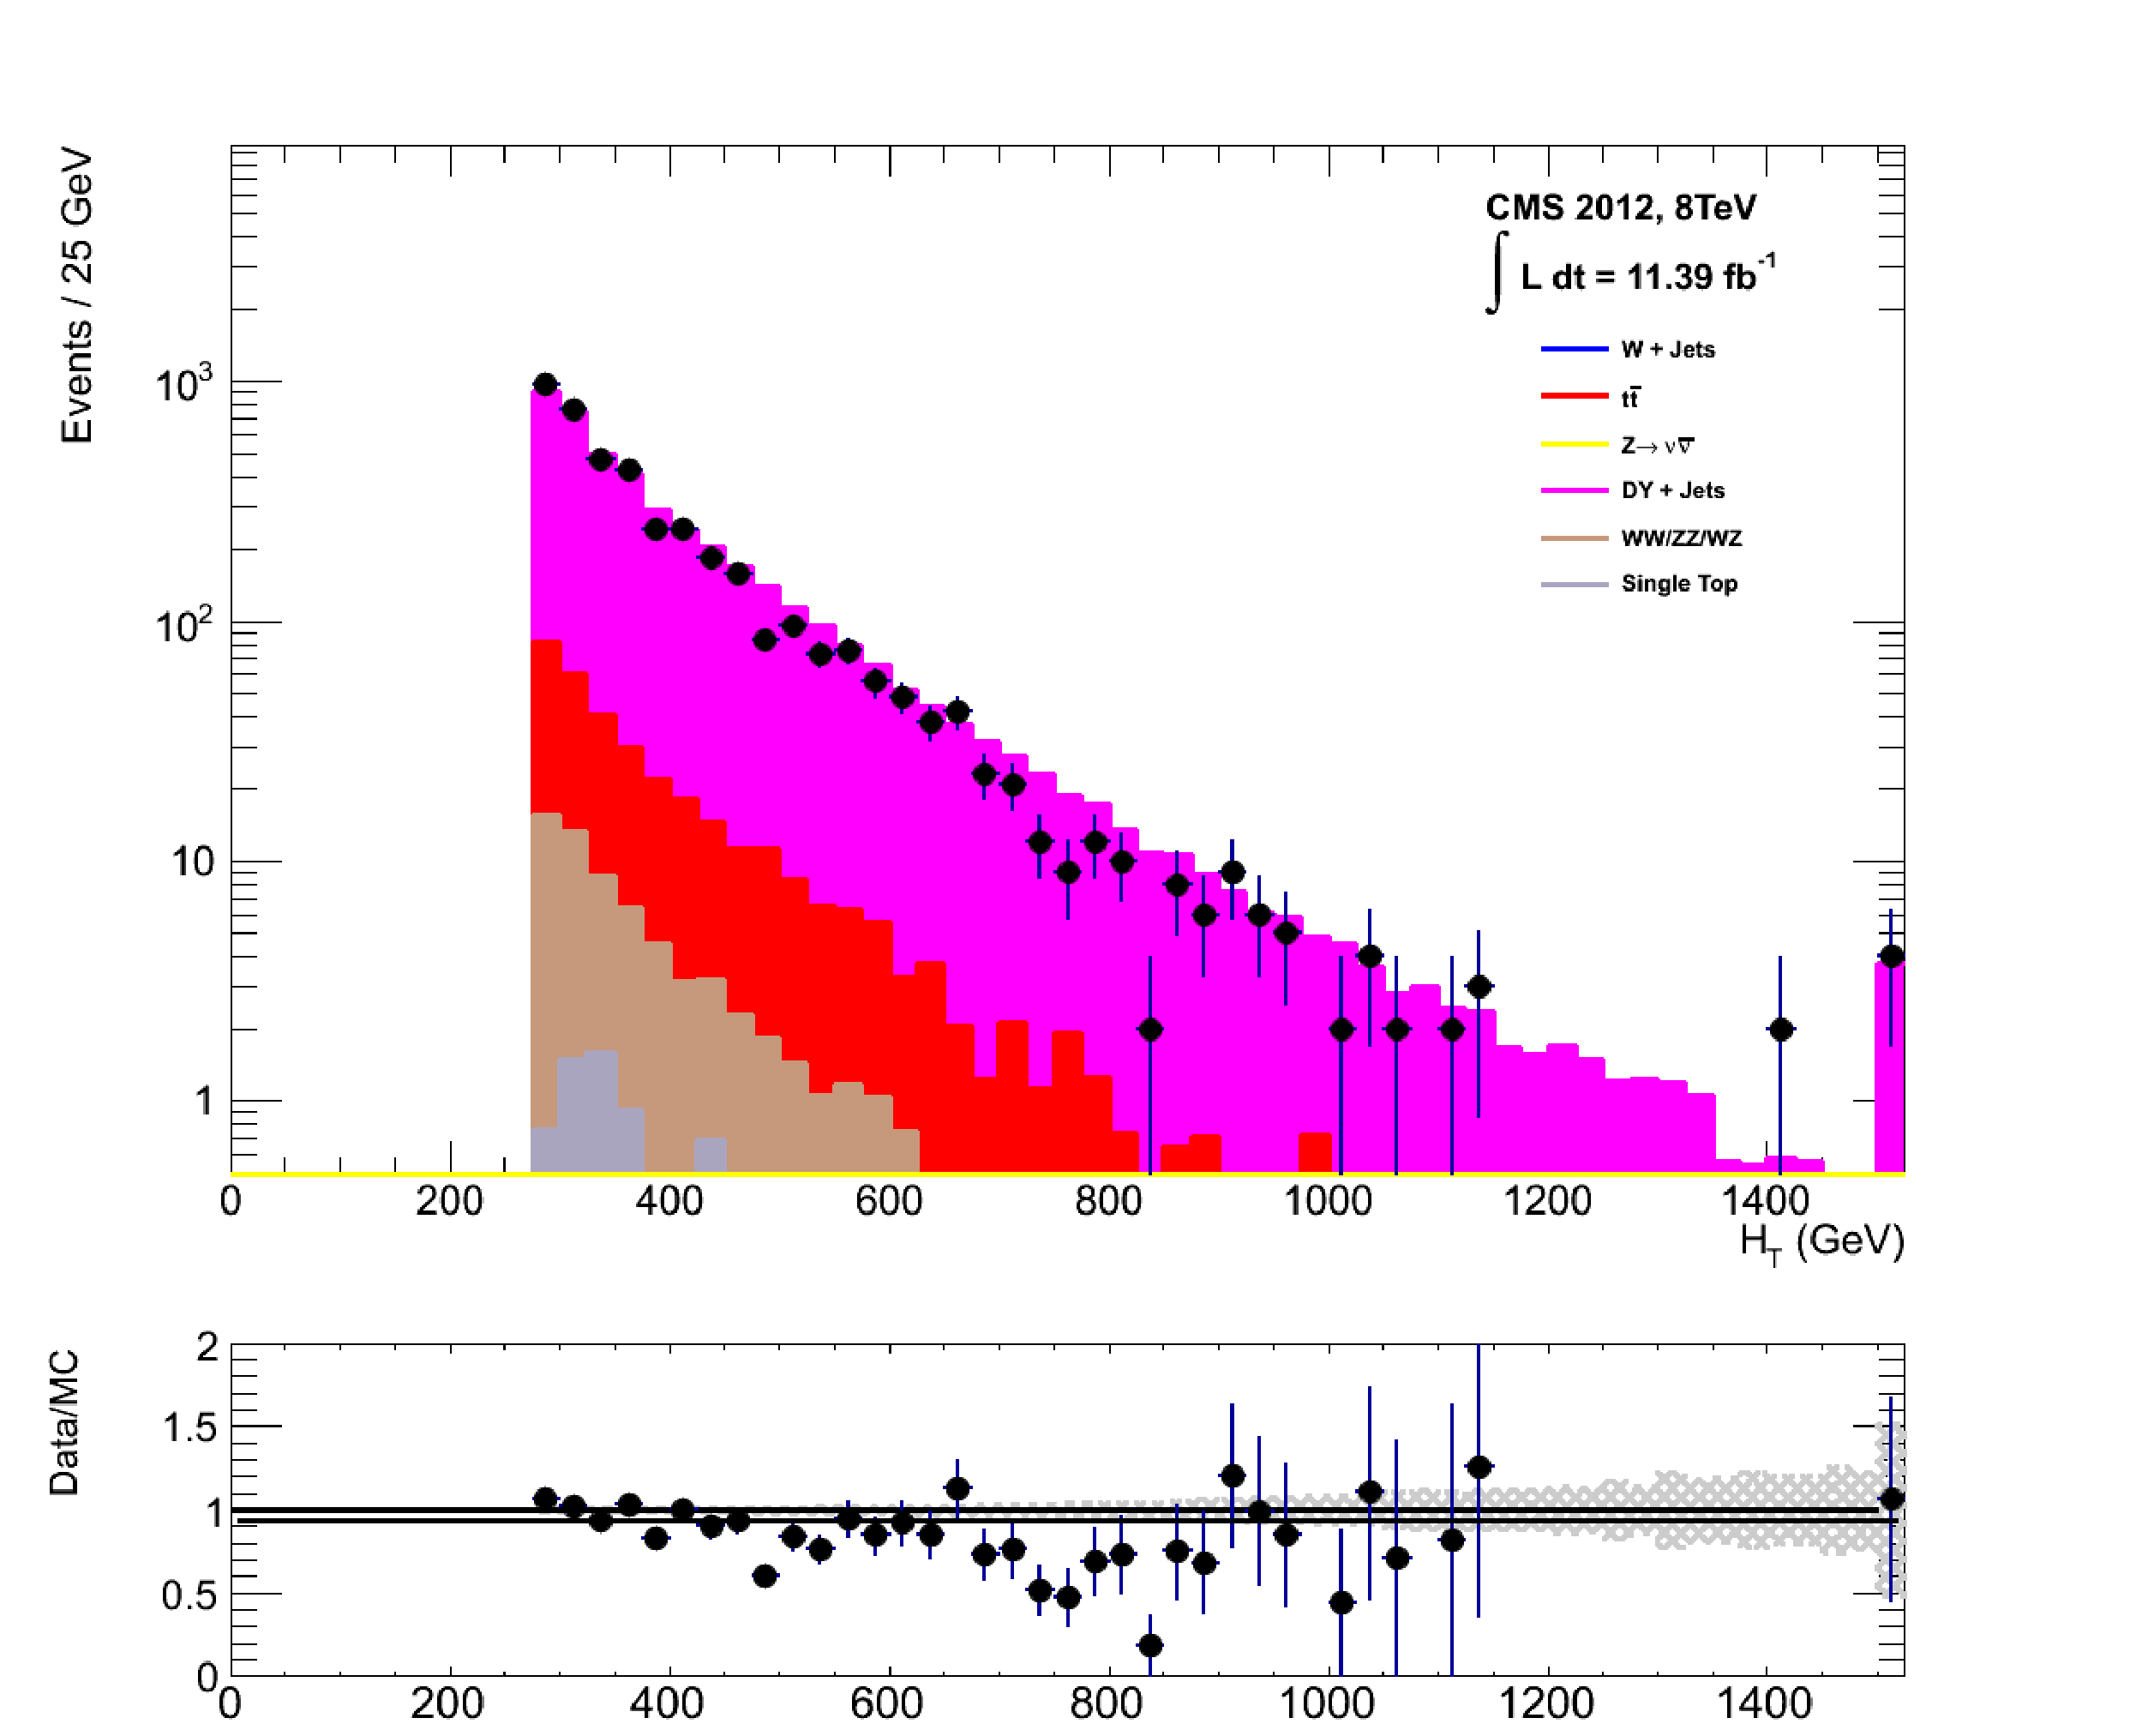
\includegraphics[width = 3.2in]{plots/dimuon_ht_datamc.pdf}
(b) \theht
\end{minipage}
\end{minipage}

\xspace

\begin{minipage}{\linewidth}
\centering
\begin{minipage}{.48\textwidth}
\centering
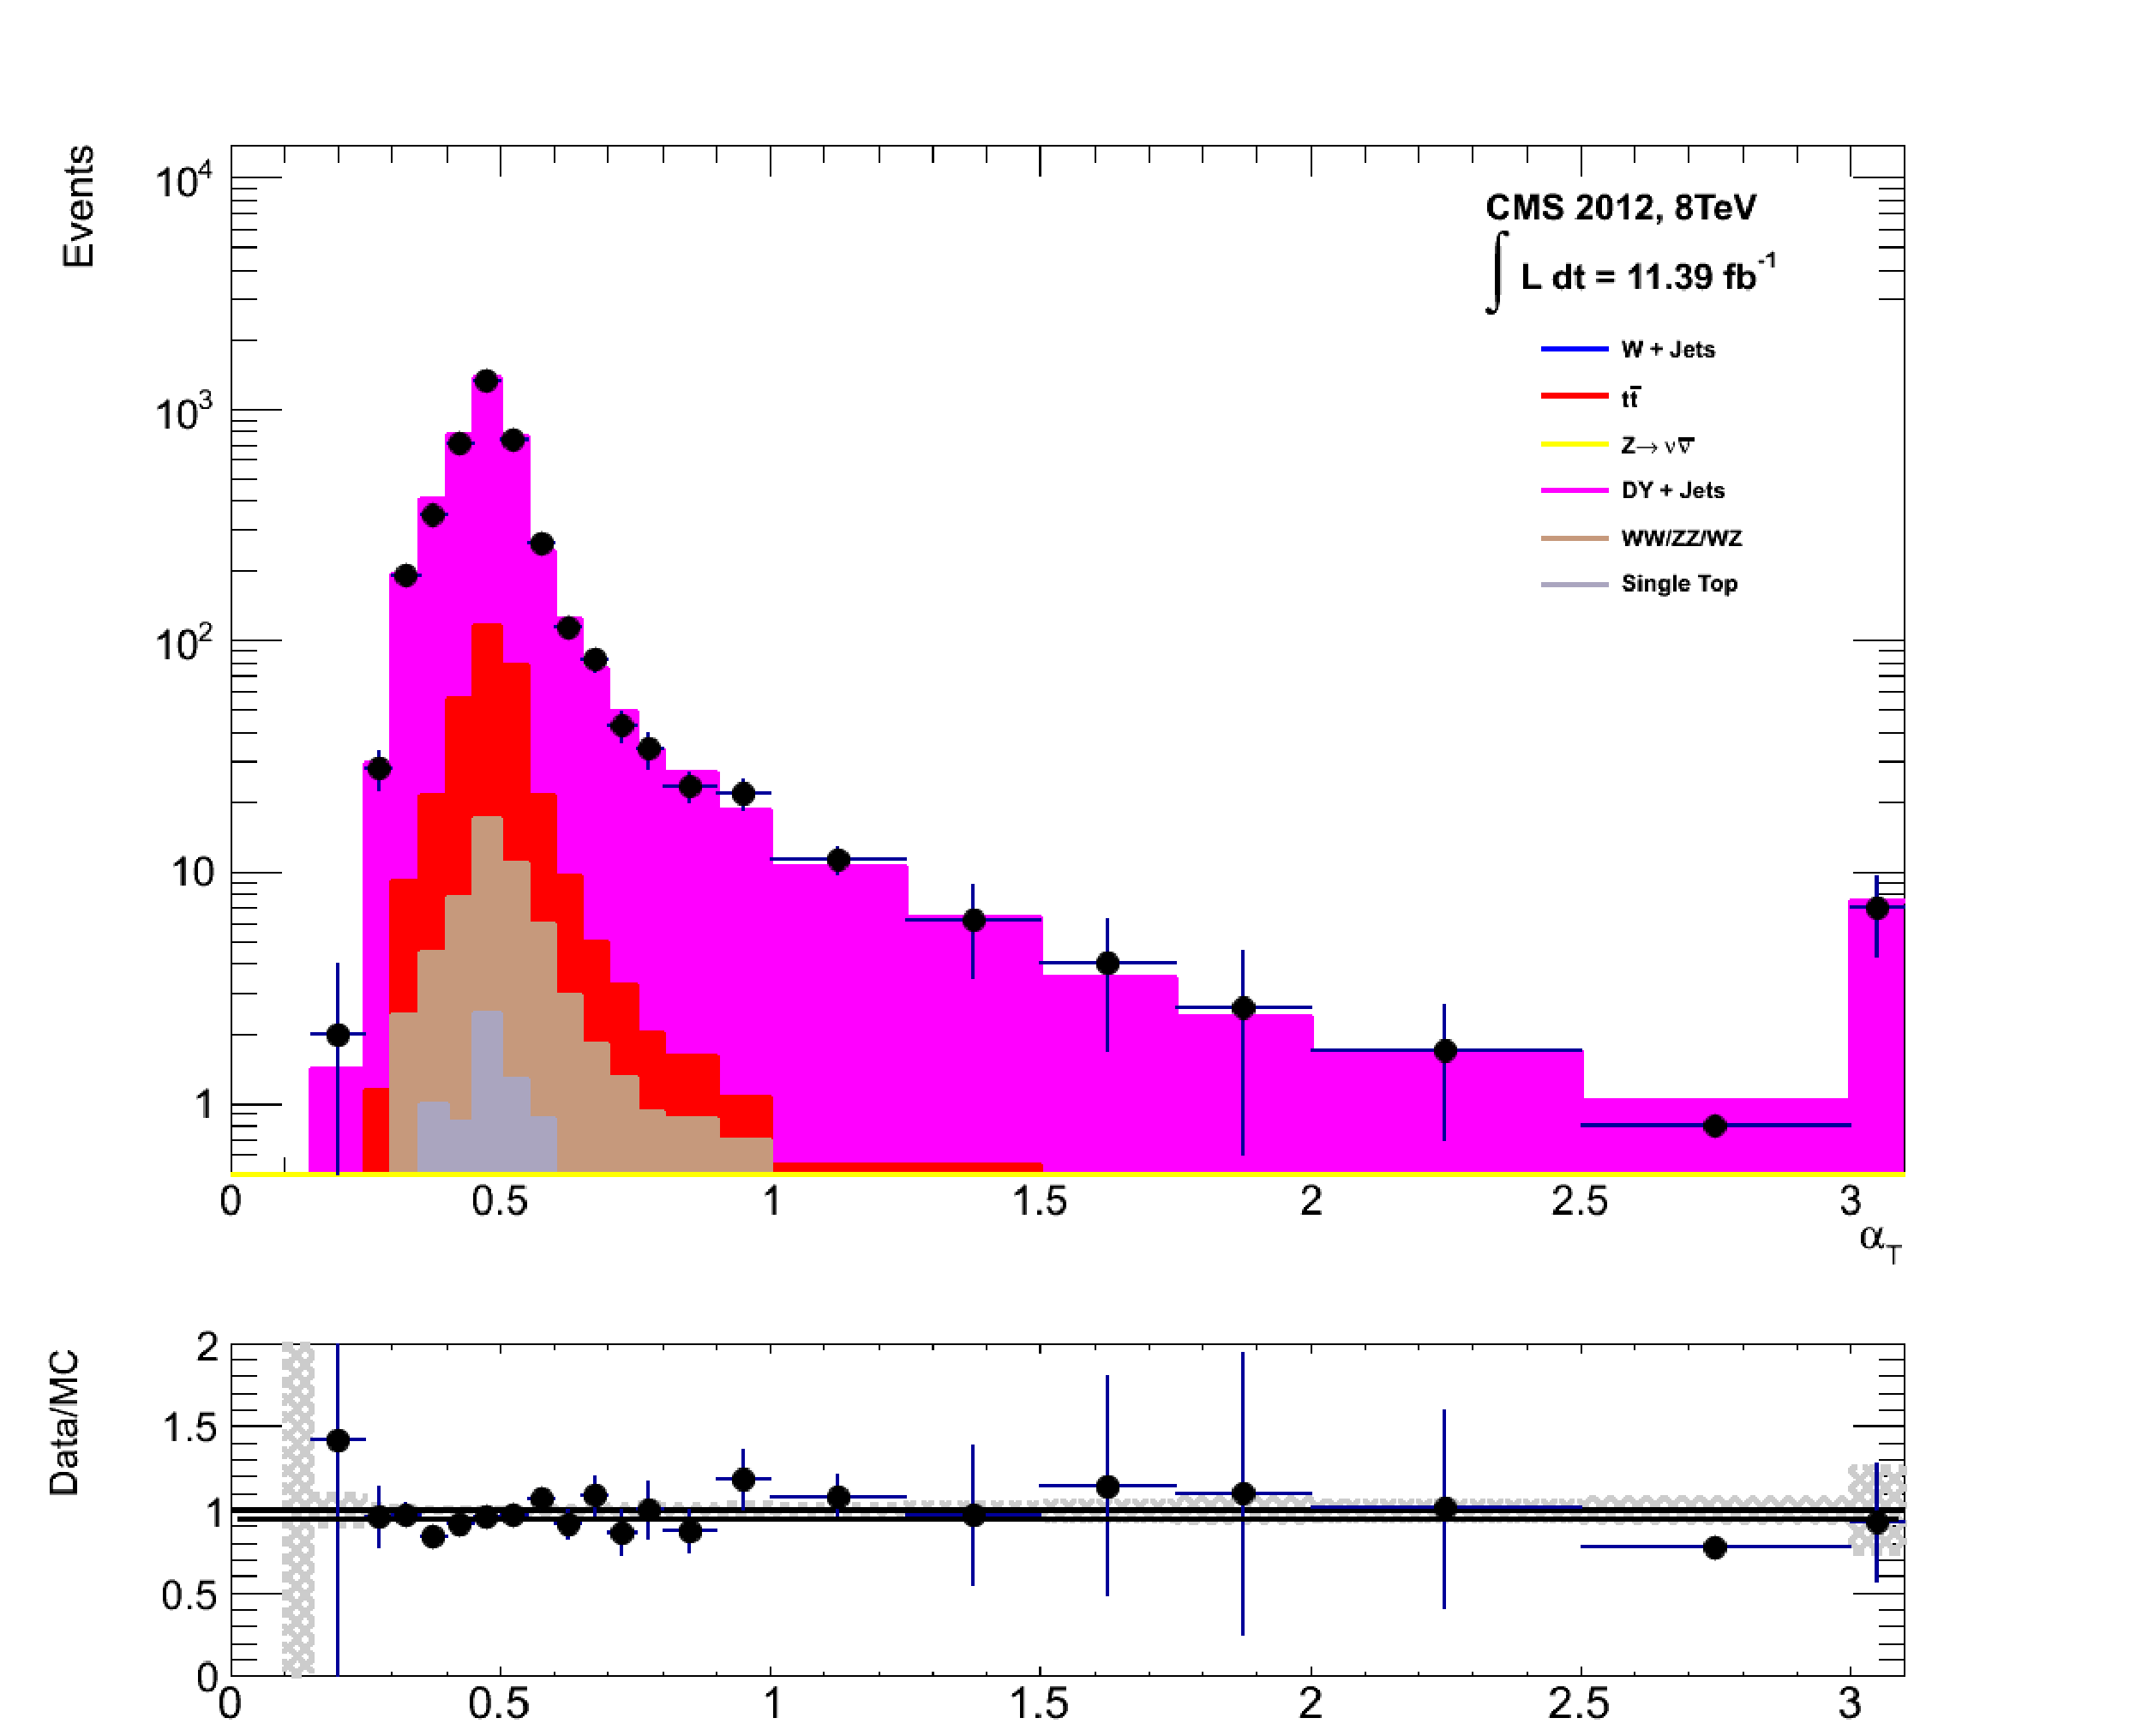
\includegraphics[width = 3.2in]{plots/dimuon_alphat_datamc.pdf}
$\text{(c}$) \alphat
\end{minipage}
\begin{minipage}{.48\textwidth}
\centering
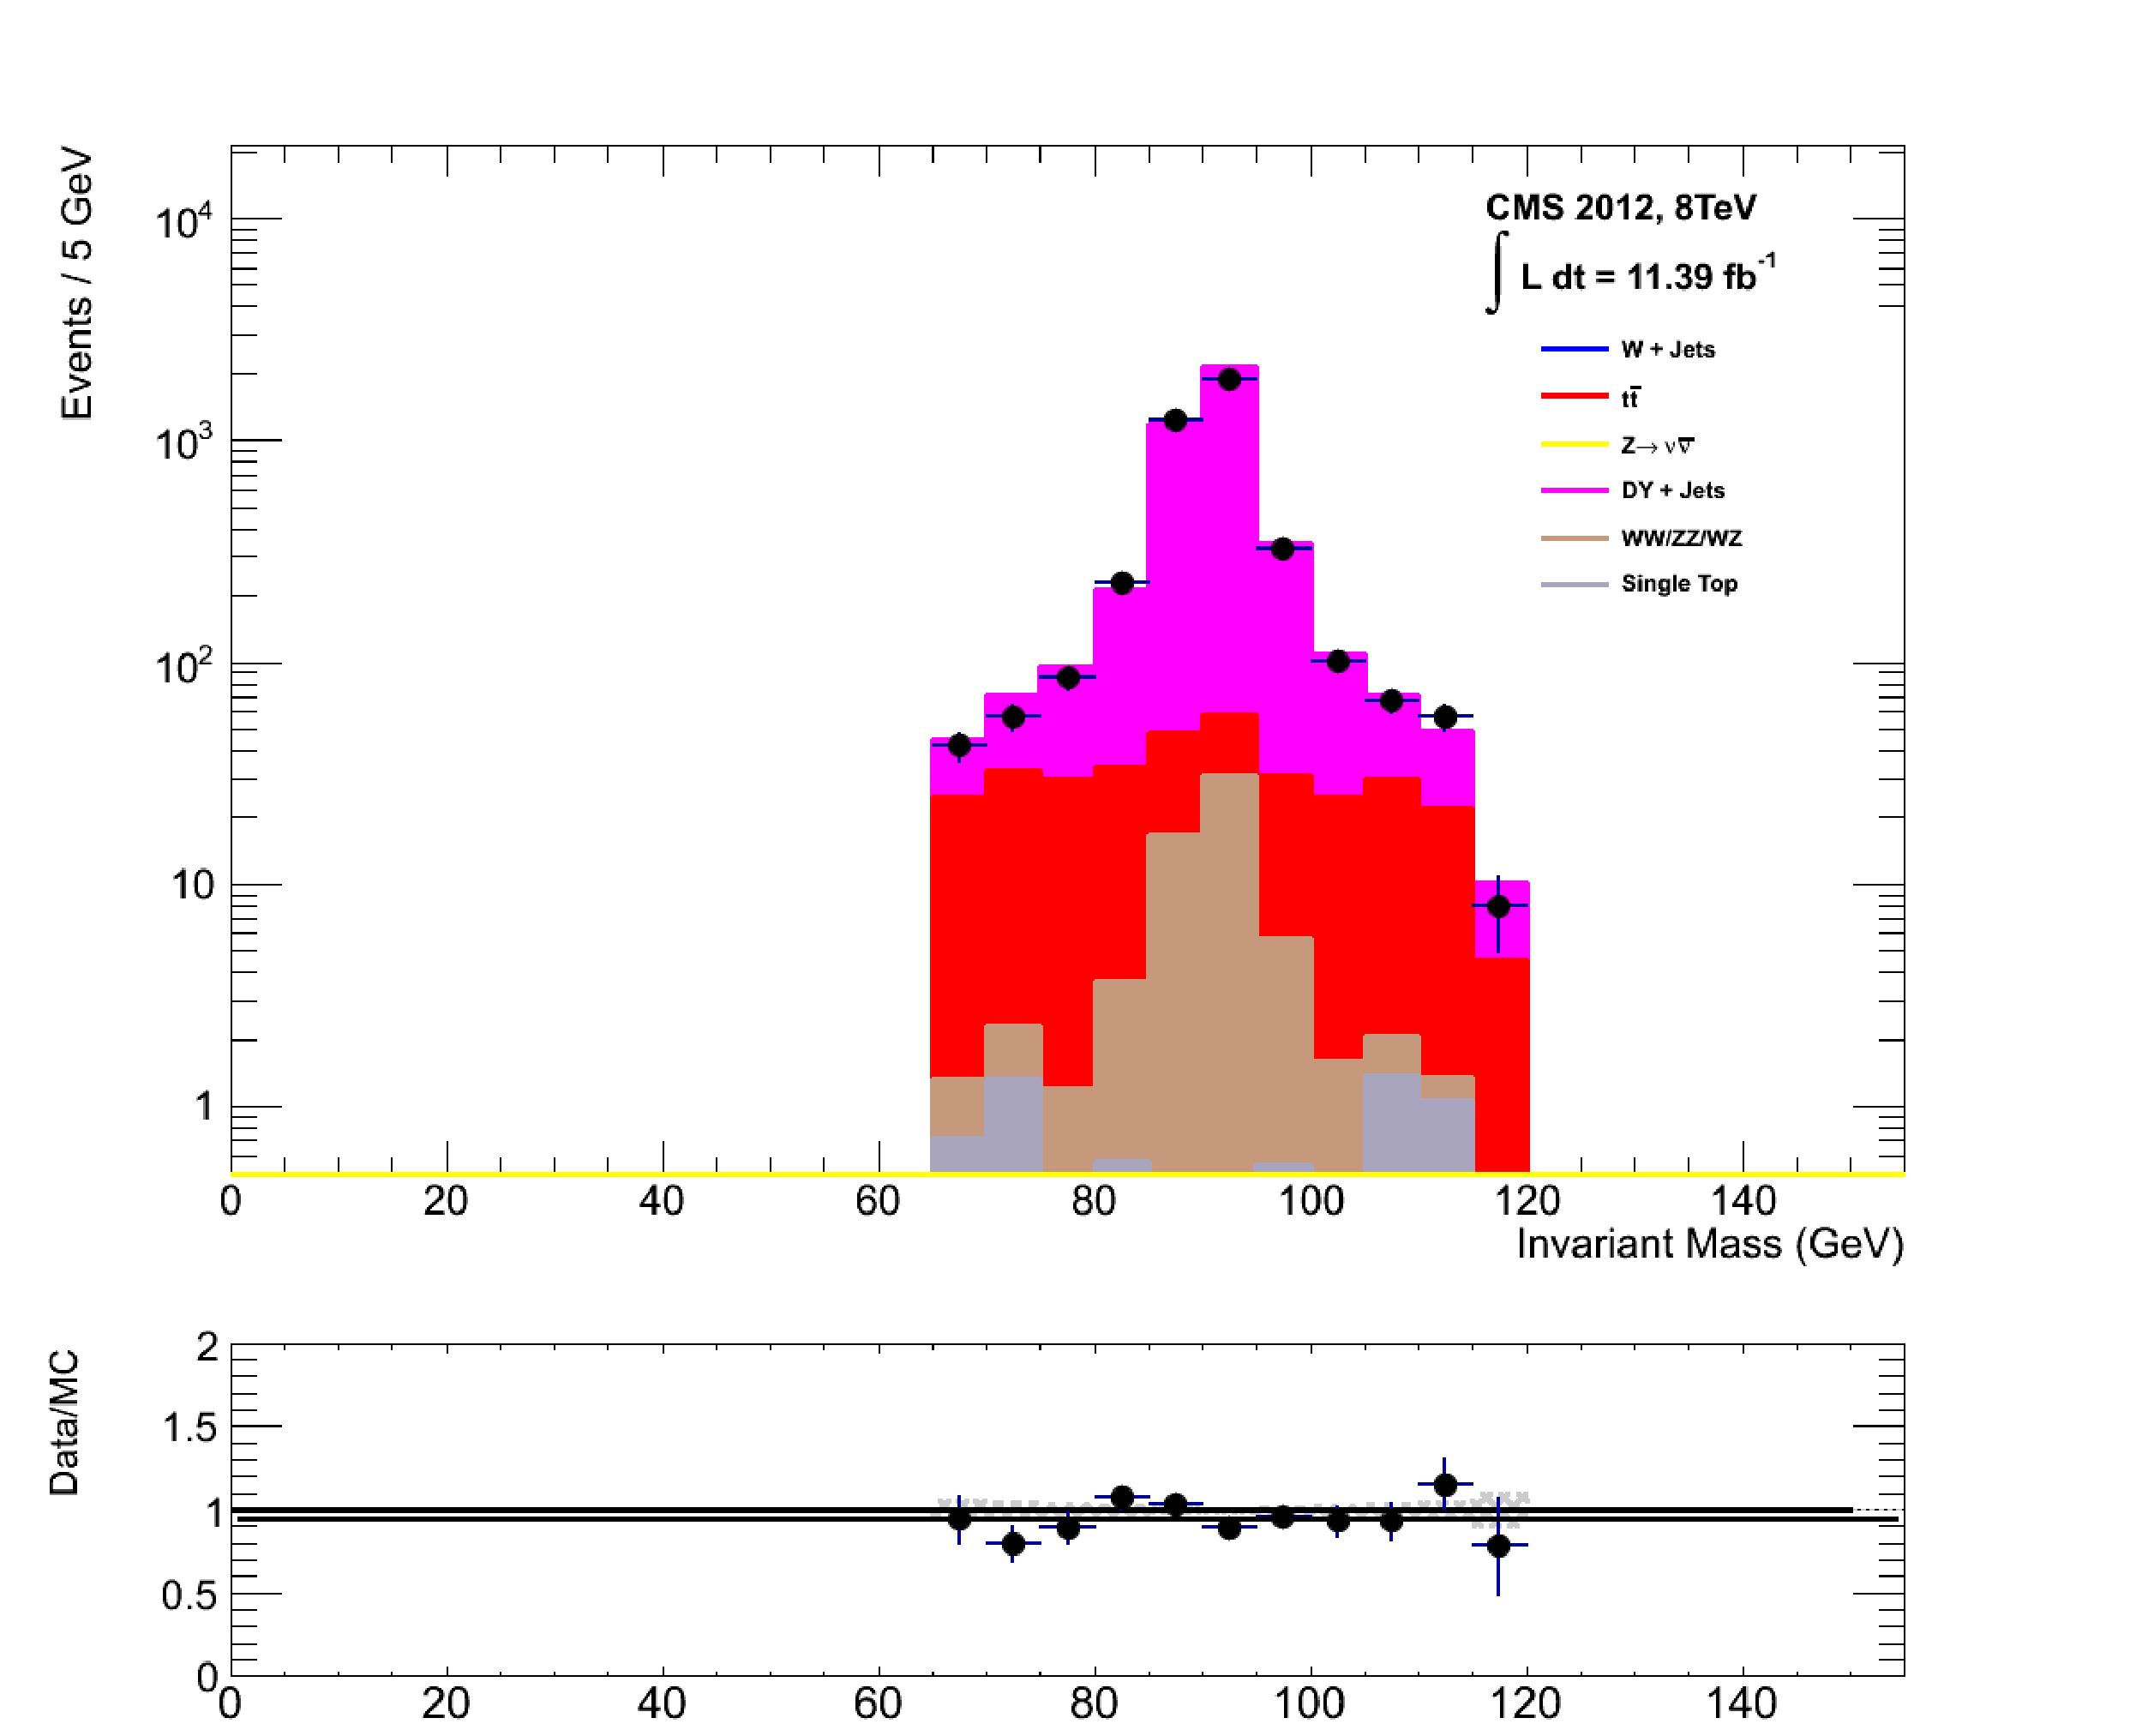
\includegraphics[width = 3.2in]{plots/dimuon_zmass_datamc.pdf}
(d) $\mu\mu$ invariant mass
\end{minipage}
\captionof{figure}[Data/MC comparisons of key variables for the \dimupjets selection.]{Data/MC comparisons of key variables for the \dimupjets selection,following the application of selection criteria and the requirements that \theht $>$ 275 \GeV. Bands represent the uncertainties due to the statistical size of the MC samples. No requirement is made upon the number of b-tagged jets or jet multiplicity in these distributions.}\label{fig:dimuonmcplots}
\end{minipage}


\item[] \textbf{The \gpjets control sample}

The \zinv + jets background is also estimated from a \gpjets control sample. When the $E_{T}$ of the photon is greater than the mass of the Z, it possesses a larger cross-section and has kinematic properties similar to those of \zinv events if the photon is ignored \cite{PhysRevD.84.114002}. 

Within the control channel, the photon is ignored for the purpose of the calculation of event level variables, and identical selection criteria to the hadronic signal region are applied. In addition the follow requirements are also made:

\begin{itemize}
\item Exactly one photon is selected, satisfying identification criteria as detailed in Table \ref{tab:photonidtable}, with a minimum \pt $> $165 \GeV to satisfy trigger thresholds and \abeta $<$ 1.45 to ensure the photon remains in the barrel of the detector.
\item A selection criteria of $\Delta R(\gamma,jet) <$ 1.0, between the photon and all jets is applied to ensure the acceptance of only well isolated \gpjets events. 
\item Given that the photon is ignored, this control sample can only be applied in the \theht region $>$ 375 \GeV, due to the trigger thresholds on the minimum \pt of the photon, and the \mht requirement of an \alphat $>$ 0.55 cut from Equation (\ref{eq:alphatmht}). This is maintained in this control sample due to contamination from QCD processes in the absence of an \alphat cut.
\end{itemize}


\begin{minipage}{\linewidth}
\centering
\begin{minipage}{.48\textwidth}
\centering
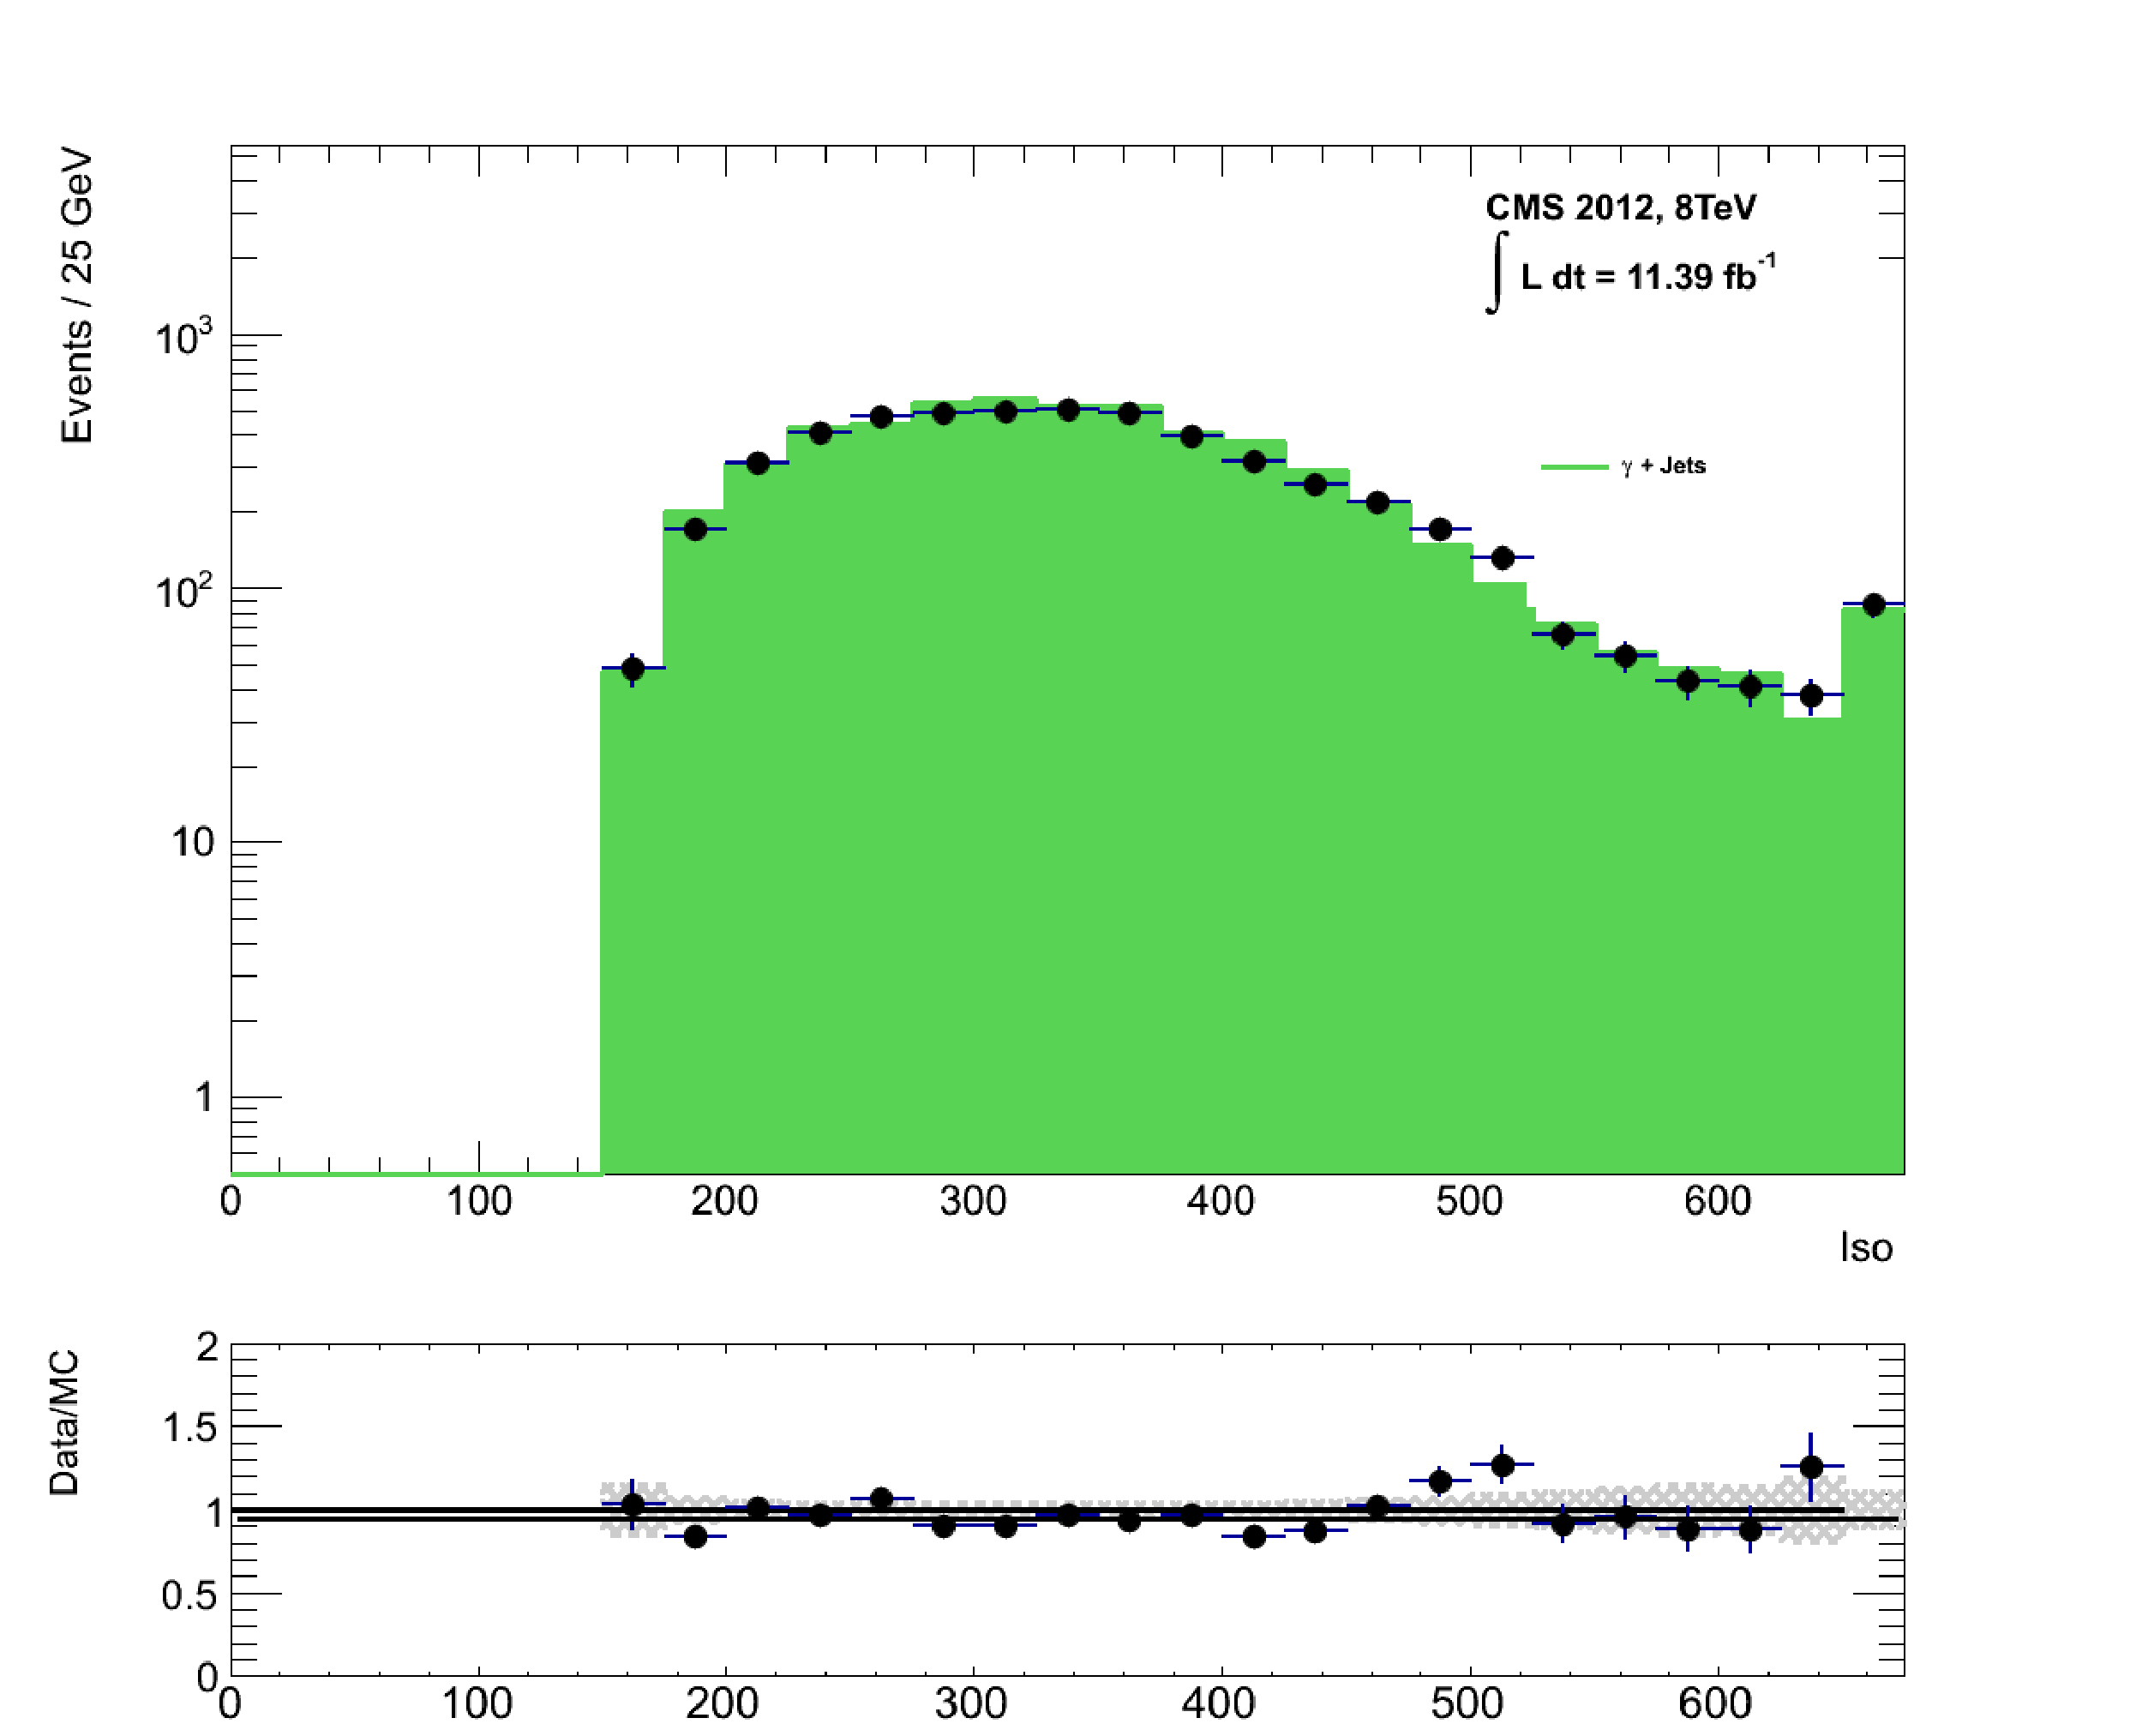
\includegraphics[width = 3.2in]{plots/photon_leadphoton_datamc.pdf}
(a) Lead Photon \pt
\end{minipage}
\begin{minipage}{.48\textwidth}
\centering
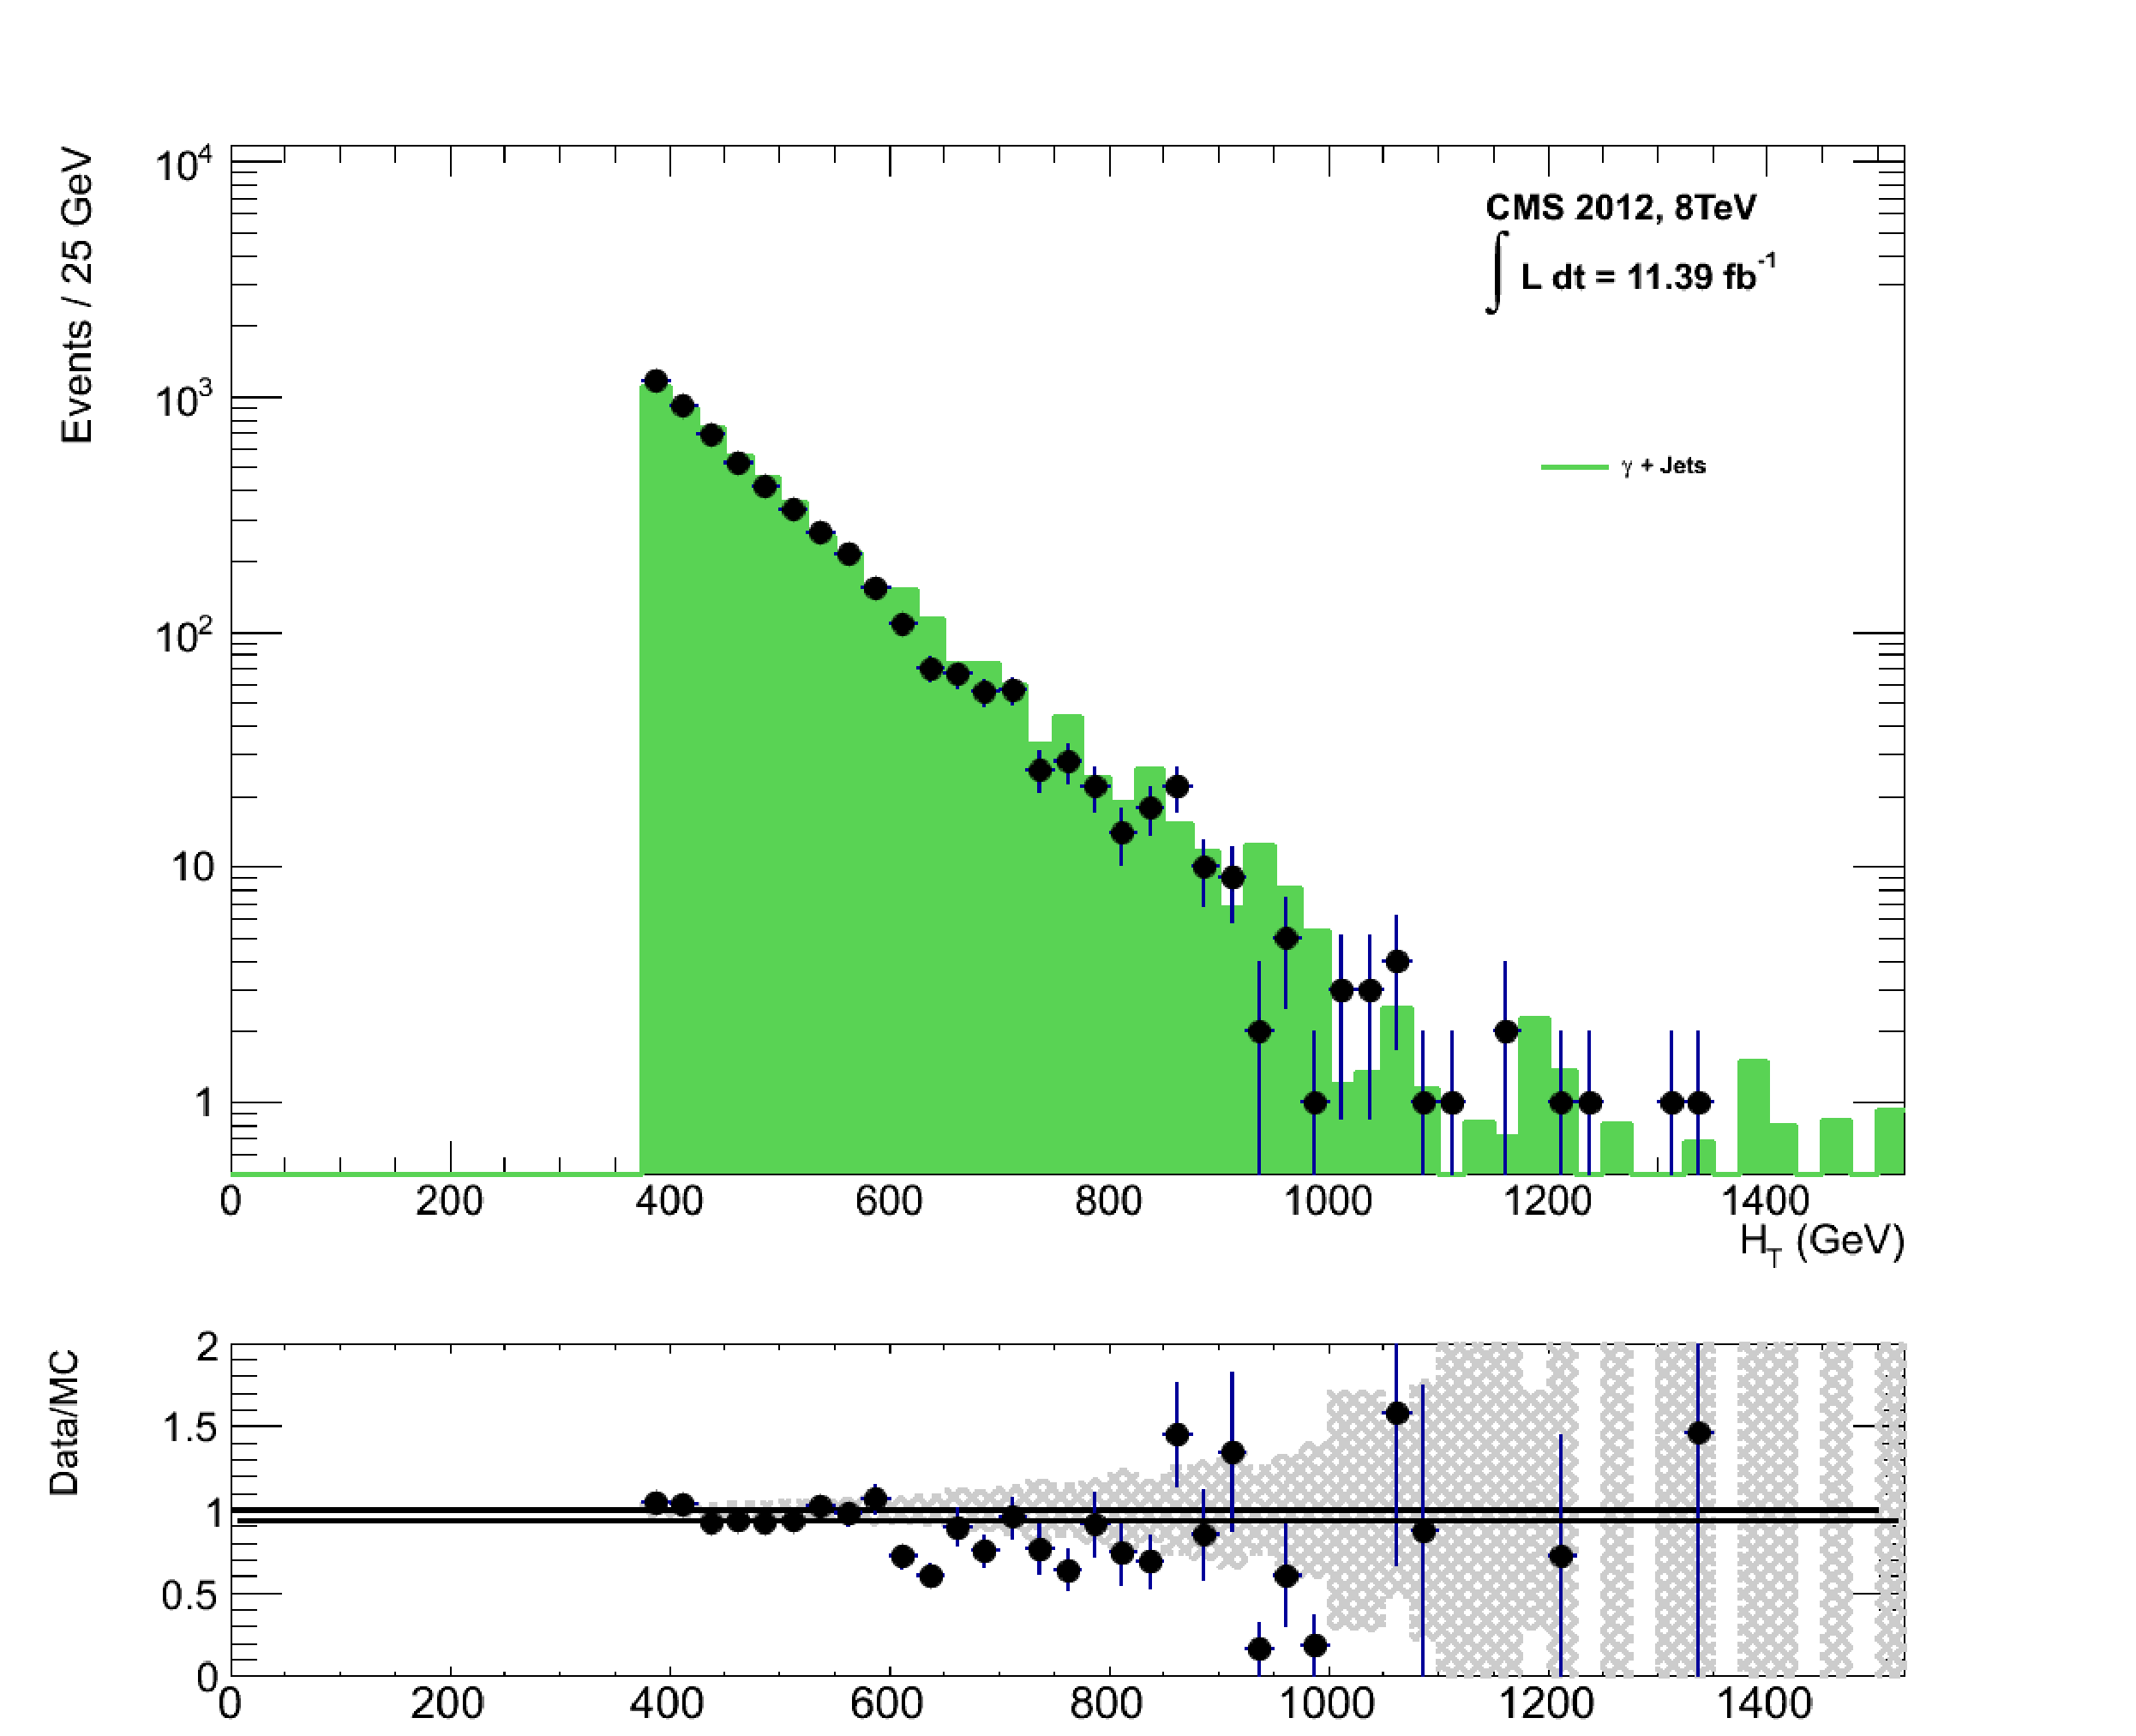
\includegraphics[width = 3.2in]{plots/photon_ht_datamc.pdf}
(b) \theht
\end{minipage}
\end{minipage}

\xspace

\begin{minipage}{\linewidth}
\centering
\begin{minipage}{.48\textwidth}
\centering
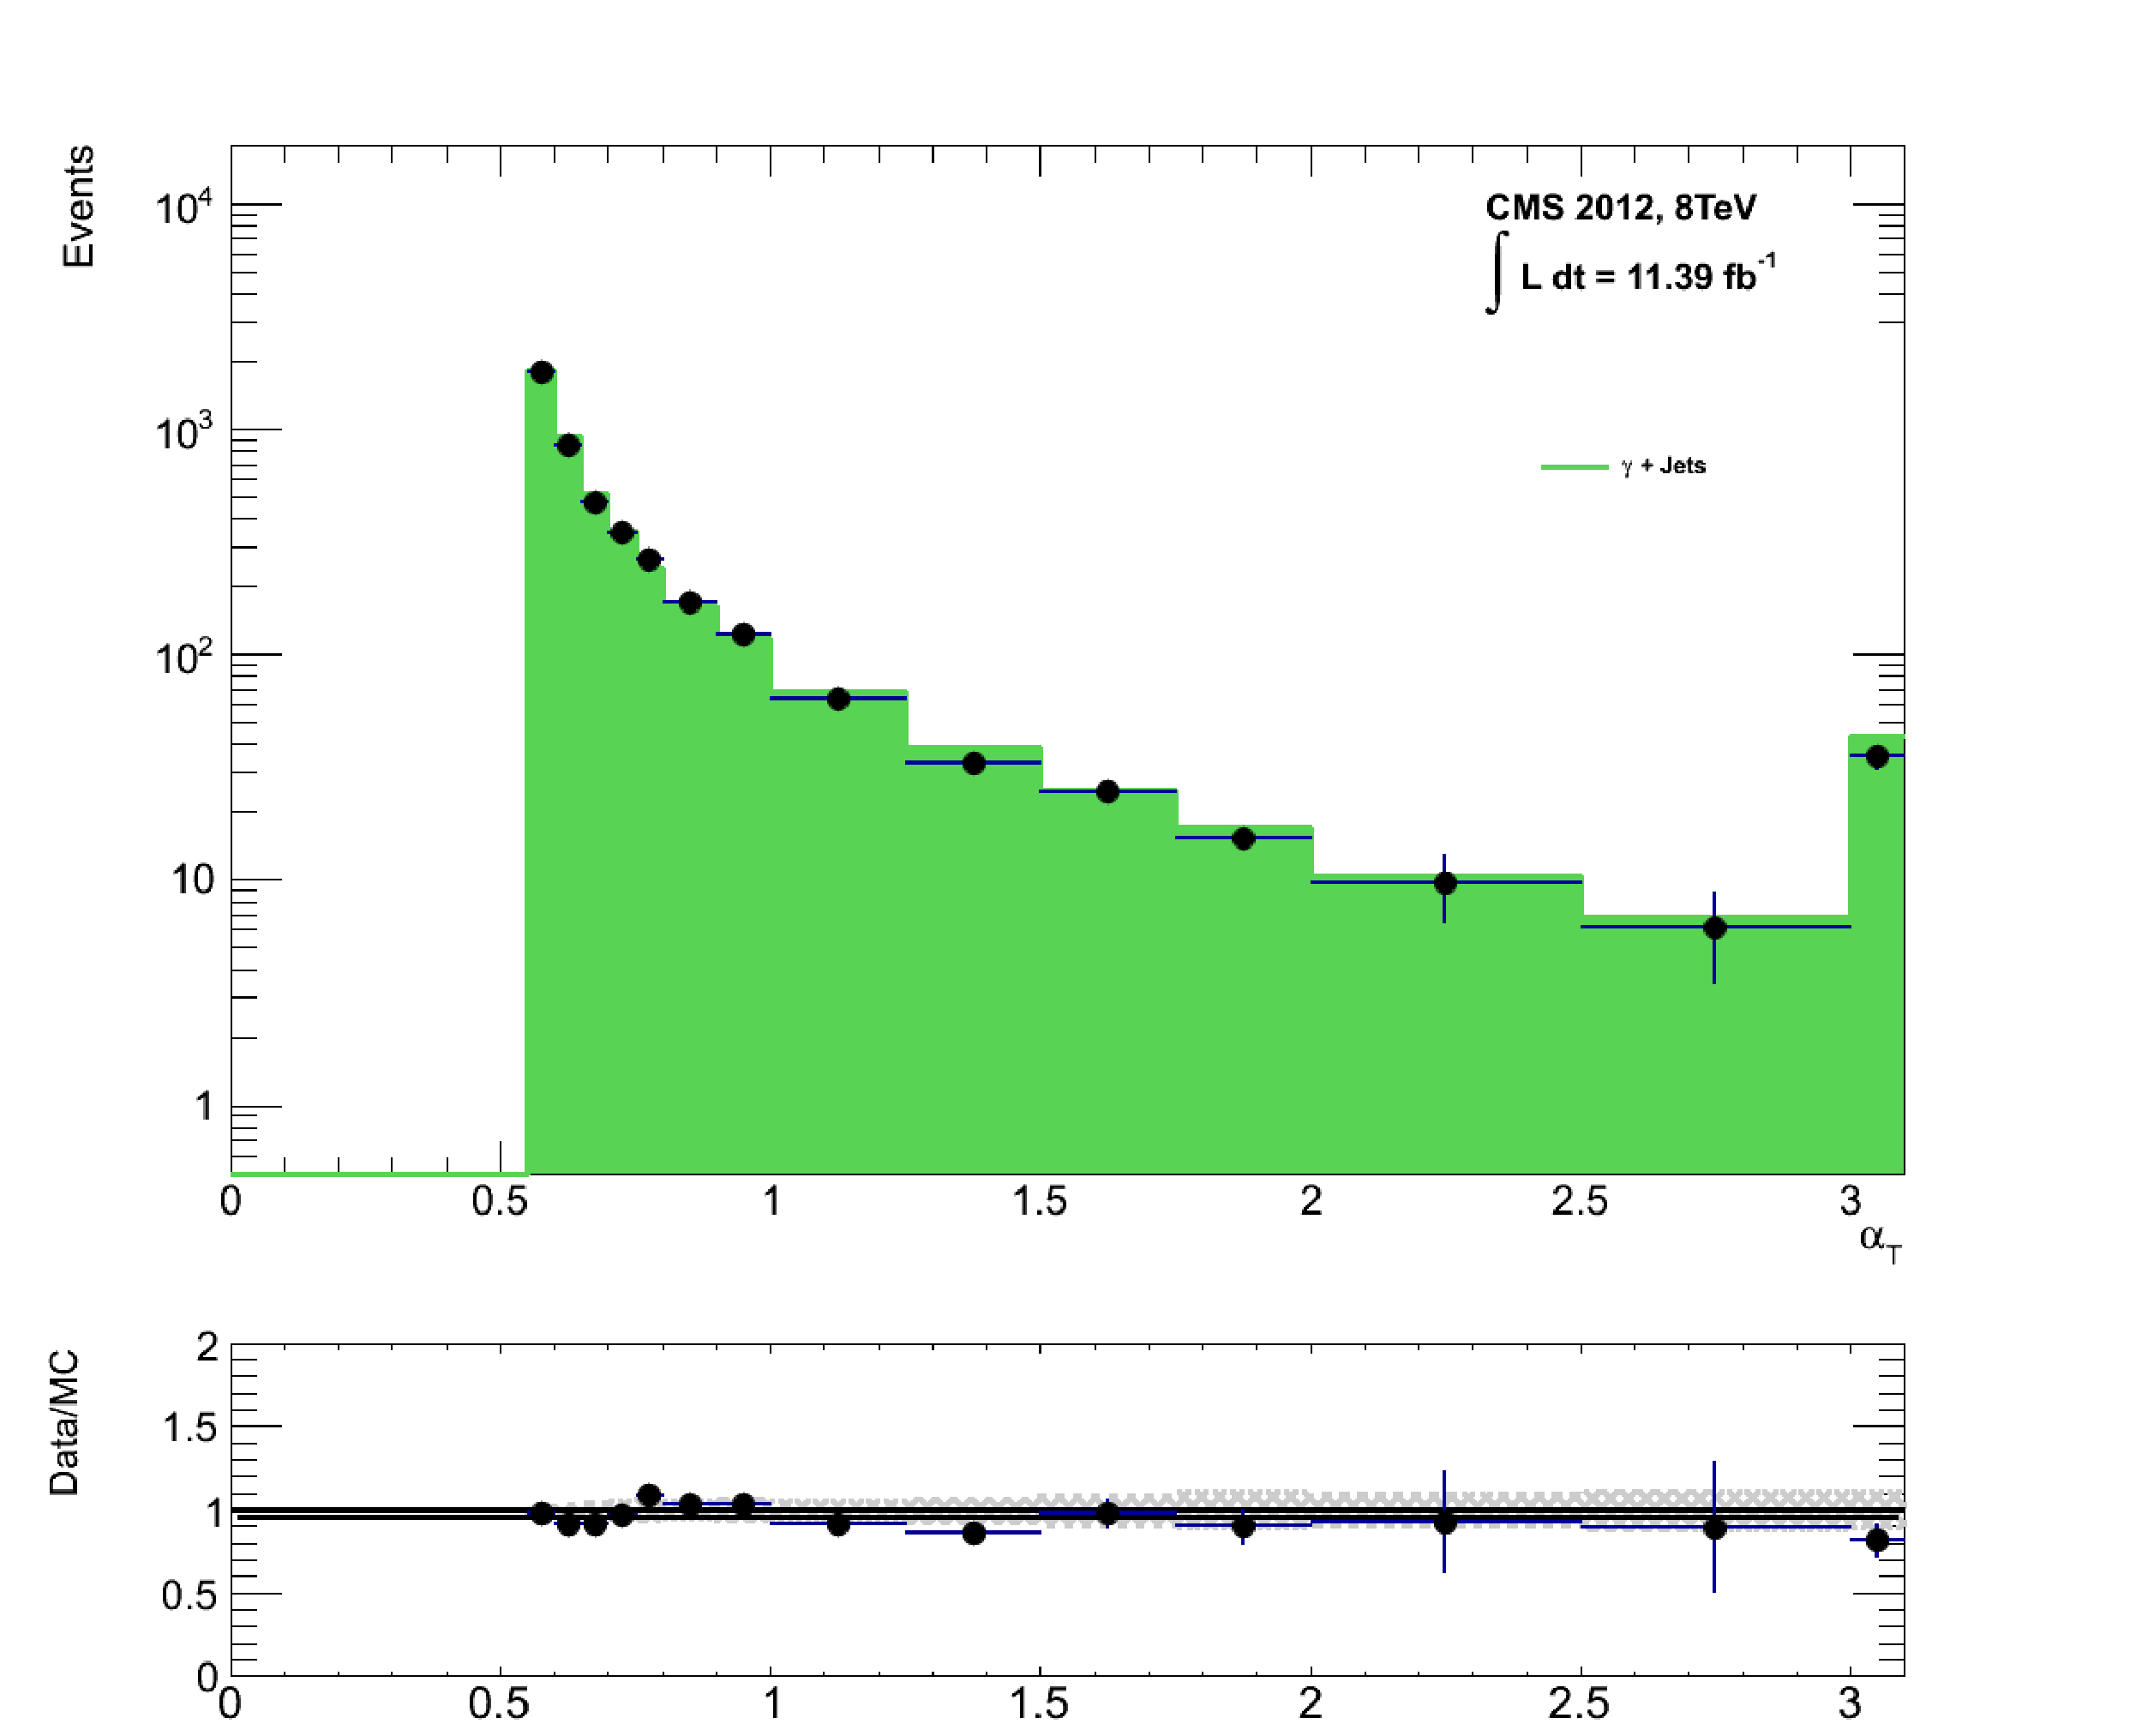
\includegraphics[width = 3.2in]{plots/photon_alphat_datamc.pdf}
$\text{(c}$) \alphat
\end{minipage}
\begin{minipage}{.48\textwidth}
\centering
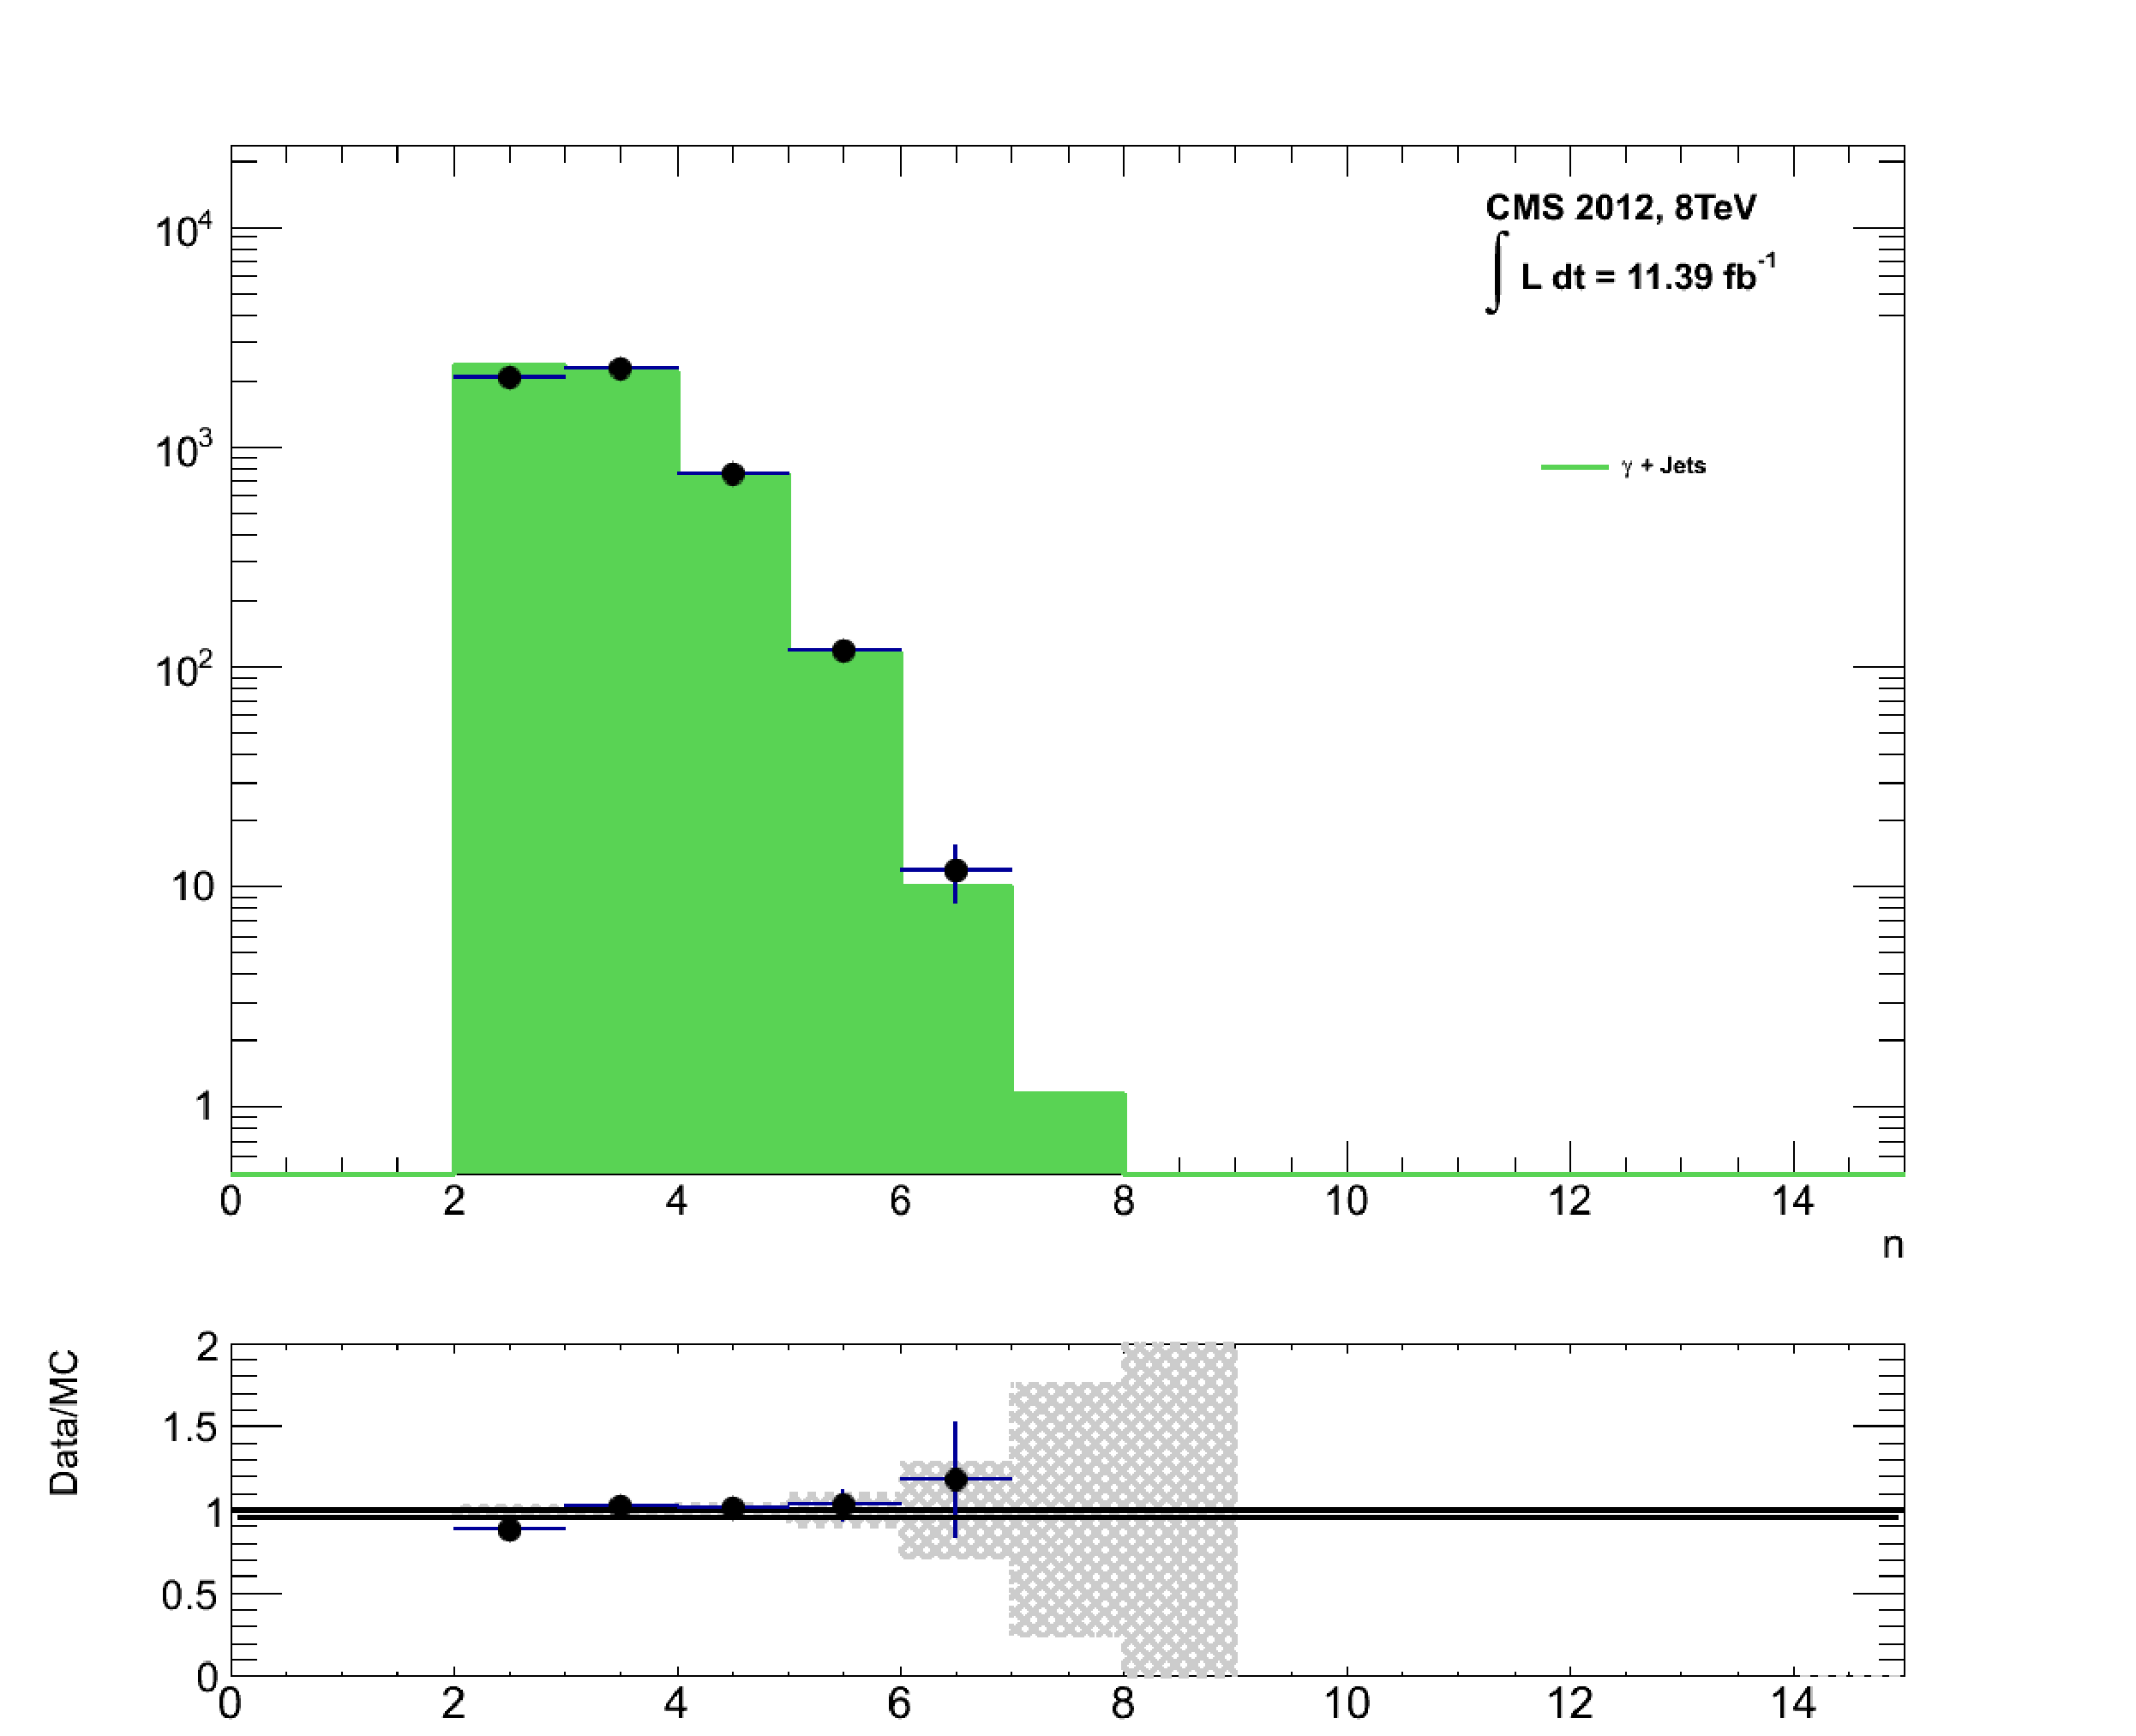
\includegraphics[width = 3.2in]{plots/photon_njet_datamc.pdf}
(d) Jet multiplicity
\end{minipage}
\captionof{figure}[Data/MC comparisons of key variables for the \gpjets selection.]{Data/MC comparisons of key variables for the \gpjets selection, following the application of selection criteria and the requirements that \theht $>$ 375 \GeV and \alphat $>$ 0.55. Bands represent the uncertainties due to the statistical size of the MC samples. No requirement is made upon the number of b-tagged jets or jet multiplicity in these distributions.}\label{fig:photonmcplots}
\end{minipage}

\end{itemize}

The selection criteria of the three control samples are defined to ensure background composition and event kinematics mirror closely the signal region. This is done in order to minimise the reliance on simulation to model correctly the backgrounds and event kinematics in the control and signal samples. 

However in the case of the \mupjets and \dimupjets samples, the \alphat requirement is relaxed in the selection criteria of these samples. This is made possible as contamination from QCD multi-jet events is suppressed to a negligible level by the other kinematic selection criteria within the two control samples, selecting pure \ac{EWK} processes. Thus in this way, the acceptance of the two muon control samples can be significantly increased, which simultaneously improves their statistical and predictive power and also dilutes the effect of any potential signal contamination. 

The modelling of the \alphat variable is probed through a dedicated set of closure tests, described in Section (\ref{subsec:sysuncertainties}), which demonstrate that the different \alphat acceptances for the control and signal samples have no significant systematic bias on the background predictions.


\subsection{Estimating the QCD Multi-jet Background}
\label{subsec:qcdbackground}

A negligible background from QCD multi-jet events within the hadronic signal region is expected due to a combination of selection requirements, and additional applied cleaning filters. However a conservative approach is still adopted and the likelihood model, see Section (\ref{subsec:htevolution}), is given the freedom to accommodate any potential QCD multi-jet contamination. 

Any potential contamination can be identified through the variable $R_{\alphat}$, defined as the ratio of events above and below the \alphat threshold value used in the analysis. This is modelled by a \theht dependant falling exponential function which takes the form,

\begin{equation}
\label{eq:qcdmodel}
R_{\alphat}(\theht) =  A_{\text{QCD}} \exp^{-k_{QCD}\theht},
\end{equation}

where the parameters A$_{\text{QCD}}$ and $k_{\text{QCD}}$ are the normalisation and exponential decay constants, respectively. 

For QCD multi-jet event topologies, this exponential behaviour as a function of \theht is expected for several reasons. The improvement of jet energy resolution at higher \theht due to higher \pt jets leads to a narrower peaked \alphat distribution, causing $R_{\alphat}$ to fall. Similarly at higher \theht values $>$ 375 \GeV, the jet multiplicity rises slowly with \theht. As shown in Figure \ref{fig:fullalphatdistribution}, at higher jet multiplicities the result of the combinatorics used in the determination of \alphat lead to more conservative \alphat values, also resulting in a narrower distribution. 

The value of the decay constant $k_{\text{QCD}}$ is constrained via measurements within data sidebands to the signal region. This is also done to validate the falling exponential assumption for QCD multi-jet topologies. The sidebands are enriched in QCD multi-jet background and defined as regions where either \alphat is relaxed or that the $R_{\text{miss}}$ cut is inverted. Figure \ref{fig:qcdcartoon} depicts the definition of these data sidebands used to constrain the value of $k_{\text{QCD}}$.

\begin{minipage}{\linewidth}
\centering
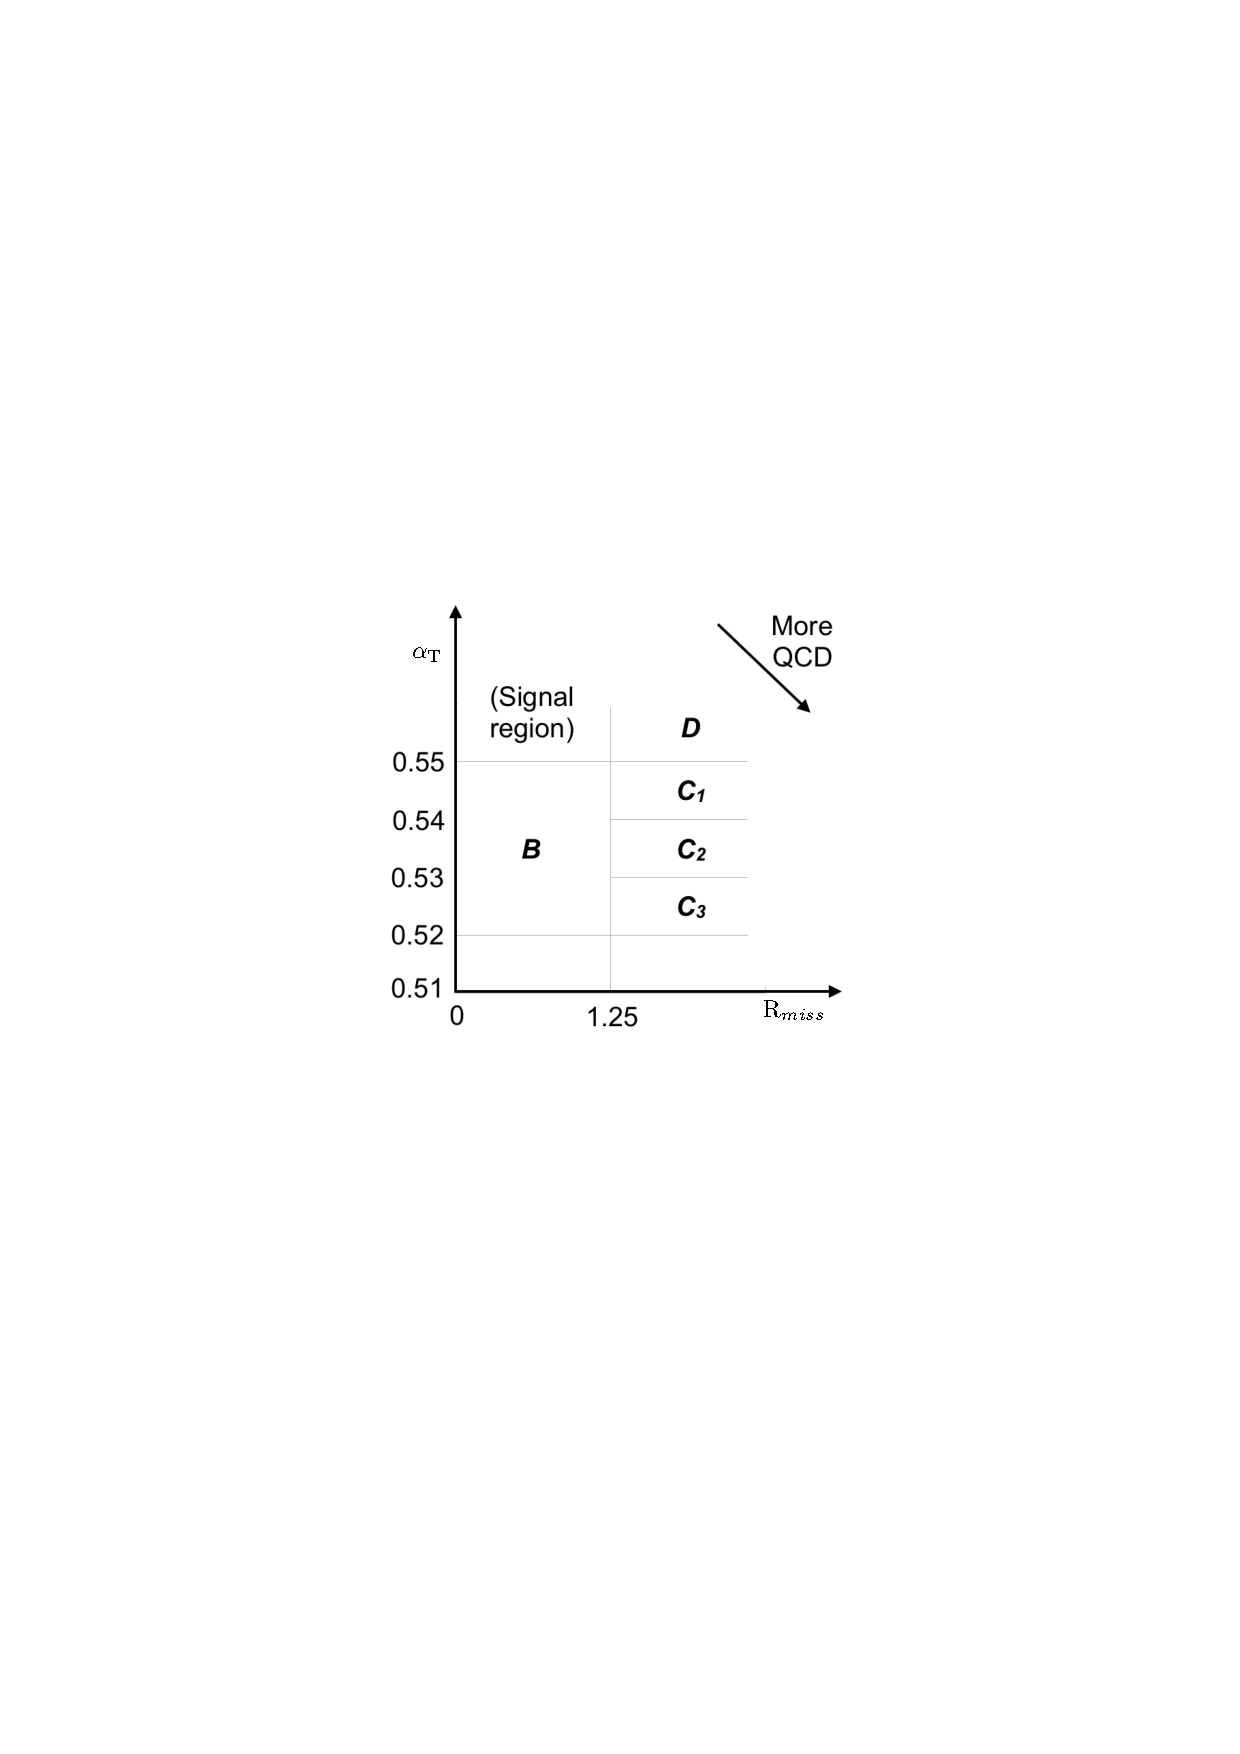
\includegraphics[width = 3.5in]{plots/qcd_cartoon.pdf}
\captionof{figure}[QCD sideband regions, used for determination of $k_{\text{QCD}}$.]{QCD sideband regions, used for determination of $k_{\text{QCD}}$.}
\label{fig:qcdcartoon}
\end{minipage}

The fit results used to determine the value of $k_{\text{QCD}}$ are shown in Appendix (\ref{app:kqcd}), for which the best fit parameter value obtained from sideband region B is determined to be $k_{\text{QCD}} = 2.96 \pm 0.64 \times 10^{-2}$ \GeV$^{-1}$. 

The best fit values of the remaining three C sideband regions are used to estimate the systematic uncertainty on the central value obtained from sideband region B. The variation of these measured values is used to determine the error on the determined central value, and is calculated to be $1.31 \pm 0.26 \times 10^{-2} \text{ \GeV}^{-1}$. This relative error of $\sim$ 20\% gives an estimate of the systematic uncertainty of the measurement to be applied to $k_{\text{QCD}}$.

Finally the same procedure is performed for sideband region D as an independent crosscheck, to establish that the value of $k_{\text{QCD}}$ extracted from a lower \alphat slice, can be applied to the signal region \alphat $>$ 0.55. The likelihood fit is performed across all \theht bins within the QCD enriched region with no constraint applied to $k_{QCD}$. The resulting best fit value for $k_{\text{QCD}}$ shows good agreement between that and the weighted mean, determined from the three C sideband regions. This demonstrates that the assumption of using the central value determined from sideband region B, to provide an unbiased estimator for $k_{\text{QCD}}$ in the signal region (\alphat $>$ 0.55) is valid.

Table \ref{tab:kqcdresults} summarises the best fit $k_{\text{QCD}}$ values determined for each of the sideband regions to the signal region.

\begin{table}[h!]
\footnotesize
\begin{center}
\begin{tabular*}{0.6\textwidth}{@{\extracolsep{\fill}}ccc}
\hline
Sideband region & $k_{\text{QCD}}$($\times 10^{-2} \GeV^{-1})$ & $p-$value\\ 
\hline\hline
B & 2.96 $\pm$ 0.64 & 0.24 \\
C$_{1}$ & 1.19 $\pm$ 0.45 & 0.93 \\
C$_{2}$ & 1.47 $\pm$ 0.37 & 0.42 \\
C$_{3}$ & 1.17 $\pm$ 0.55 & 0.98 \\
\cline{1-3}
C(weighted mean) & 1.31 $\pm$ 0.26 & - \\
D(likelihood fit) & 1.31 $\pm$ 0.09 & 0.57 \\
\end{tabular*}
\end{center}
\caption[Best fit values for the parameters $k_{\text{QCD}}$ obtained from sideband regions B,C$_{1}$,C$_{2}$,C$_{3}$. ]{Best fit values for the parameters $k_{\text{QCD}}$ obtained from sideband regions B,C$_{1}$,C$_{2}$,C$_{3}$. The weighted mean is determined from the three measurements made within sideband region C. The maximum likelihood value of $k_{\text{QCD}}$ given by the simultaneous fit using sideband region D. Quotes errors are statistical only. }
\label{tab:kqcdresults}
\end{table}


\section{Trigger Strategy}
\label{subsec:triggerstrategy}

A cross trigger based on the \theht and \alphat values of an event, is used with varying thresholds across \theht bins to record the events used in the hadronic signal region. The \alphat legs of the \htalphat triggers used in the analysis, are chosen to suppress QCD multi-jet events and control trigger rate, whilst maintaining signal acceptance. To maintain an acceptable rate for these analysis triggers, only calorimeter information is used in the reconstruction of the \theht sum, leading to the necessity for Calo jets to be used within the analysis. 

A single object prescaled \texttt{HT} trigger is used to collect events for the hadronic control region, described above in Section (\ref{subsec:qcdbackground}).

The performance of the \alphat and \theht triggers used to collect data for the signal and hadronic control region is measured with respect to a reference sample collected using the muon system. This allows measurement of both the Level 1 seed and higher level triggers simultaneously, as the reference sample is collected independently of any jet requirements. 

The selection for the trigger efficiency measurement is identical to that described in Section (\ref{subsec:eventselection}), with the requirement of exactly one well identified muon with \pt $>$ 30 \GeV. This muon is then subsequently ignored.  

The efficiencies measured for the \htalphat triggers in each individual \theht and \alphat leg, is summarised in Table \ref{tab:trigeffs} for each \theht category of the analysis.

\begin{table}[h!]
\footnotesize
\begin{center}
\begin{tabular*}{0.6\textwidth}{@{\extracolsep{\fill}}ccc}
\hline
\theht range (\GeV) & $\epsilon$ on \theht leg (\%) & $\epsilon$ on \alphat leg (\%) \\ 
\hline\hline
275-325 & $87.7^{+1.9}_{-1.9}$ & $82.8^{+1.0}_{-1.1}$ \\
325-375 & 90.6$^{+2.9}_{-2.9}$ & 95.9$^{+0.7}_{-0.9}$ \\
375-475 & 95.7$^{+0.1}_{-0.1}$ & 98.5$^{+0.5}_{-0.9}$ \\
475-$\infty$ & 100.0$^{+0.0}_{-0.0}$ & 100.0$^{+0.0}_{-4.8}$ \\
\end{tabular*}
\end{center}
\caption[Measured efficiencies of the \theht and \alphat legs of the HT and \htalphat triggers in independent analysis bins.]{Measured efficiencies of the \theht and \alphat legs of the \texttt{HT} and \htalphat triggers in independent analysis bins. The product of the two legs gives the total efficiency of the trigger in a given offline \theht bin.}
\label{tab:trigeffs}
\end{table}

Data for the control samples of the analysis, detailed in Section (\ref{subsec:controlsampledefinition}), are collected using a single object photon trigger for the \gpjets sample, and a single object muon trigger for both the \mupjets and \dimupjets control samples. 

The photon trigger is measured to be fully efficient for the threshold $\pt^{\text{photon}} > 150$ \GeV, whilst the single muon efficiency satisfying $\pt^{\text{muon}} > 30$ \GeV is measured to have an efficiency of (88$\pm$2)\% that is independent of \theht. In the case of the \dimupjets control sample, the efficiency is measured to be (95$\pm$2)\% for the lowest \theht bin, rising (due to the average \pt of the second muon in the event increasing at larger \theht)
to (98$\pm$2)\% in the highest \theht category. 

\section{Measuring Standard Model Process Normalisation Factors via \theht Sidebands}
\label{subsec:mckfactors}

The theoretical cross-sections of different \ac{SM} processes at \acf{NNLO} and the number of available simulated events generated for a particular process, is typically used to determine the appropriate normalisation for a simulation sample. However within the particular high-\theht and high-\met corners of kinematic phase space probed within this search, the theoretical cross sections for various processes are far less well understood. 

To mitigate the problem of theoretical uncertainties and arbitrary choices of cross sections, the normalisation of the simulation samples are determined through the use of data sidebands. The sidebands are used to calculate sample specific correction factors (k-factors), that are appropriate for the \theht-\met phase space covered by this analysis. 

They are defined within the \mupjets and \dimupjets control sample, by the region 200$<$ \theht$<$275, using the same jet \pt thresholds as the adjacent first analysis bin. Individual \ac{EWK} processes are isolated within each of these control samples via requirements on jet multiplicity and the requirement on b-tag multiplicity, summarised in Table \ref{tab:mckfactors}. The purity of the samples are typically $>$ 90\% with any residual contamination subtracted prior to determination of the correction factors. The resultant k-factor for each process is determined by then taking ratio of the data yield over the expectation from simulation in the sideband. Subsequently these k-factors are then applied to the processes within the phase space of the analysis.

 \begin{table}[h!]
\begin{center}
\footnotesize
\begin{tabular*}{0.95\textwidth}{@{\extracolsep{\fill}}llccc}
\hline
Process & Selection & Observation & MC expectation & k-factor \\
\hline\hline
W + jets & \mupjets, n$_{b}$=0, n$_{jet}$ = 2,3 &26950 & 29993.2 $\pm$ 650.1 & 0.90 $\pm$ 0.02 \\
$Z \rightarrow \mu\mu$ + jets & \dimupjets, n$_{b}$=0, n$_{jet}$ = 2,3 & 3141 & 3402.0 $\pm$ 43.9 & 0.92 $\pm$ 0.02 \\
\ttbar & \mupjets, n$_{b}$=2, n$_{jet}$ = $\geq$4 & 2190 & 1967.8 $\pm$ 25.1 & 1.11 $\pm$ 0.02 \\
\end{tabular*}
\end{center}
\caption[k-factors calculated for different \ac{EWK} processes.]{k-factors calculated for different \ac{EWK} processes. All k-factors are derived relative to theoretical cross-sections calculated in \ac{NNLO}. The k-factors measured for the Z$\rightarrow \mu\mu$ + jets processes, are also applied to the \zinv + jets and \gpjets simulation samples.}\label{tab:mckfactors}
\end{table}

It is worth pointing out that these correction factors have a negligible effect when providing a background estimation for the signal region. The \ac{TF}s used in the analysis are found to be unaffected by application of these k-factors due to the similarity in the background composition of the control and signal regions. However when systematic uncertainties are determined in Section (\ref{subsec:sysuncertainties}), the closure tests performed are sensitive to these corrections when extrapolations between different $n_{b}^{reco}$ and $n_{\text{jet}}$ categories are performed.


\section{Determining Monte Carlo Simulation Yields with Higher Statistical Precision}
\label{subsec:backgroundestimation}

Reconstructing events from \ac{EWK} processes with many b-tagged jets ($\geq$3), \nbreco, is largely driven by the mis-tagging of light jets within the event. This is clear when considering the main \ac{EWK} backgrounds in the analysis, such as \ttbar + jets events, which typically contain two underlying b-quarks in the final state from the decay of the top quarks. Conversely W + jets and Z$\rightarrow \mu\mu$ + jets events will typically contain no underlying b-quarks in its final state.

When the expectation for the number of \nbreco jets is taken directly from simulation, the statistical uncertainty at large reconstructed b-tagged jet multiplicities becomes relatively large. One approach to reduce this uncertainty is to use the information encoded throughout all events in the simulation sample, to measure each of the following four ingredients:

\begin{enumerate}
\item the averaged b-tagging efficiency in the event selection,
\item the averaged charm-tagging efficiency in the event selection,
\item the averaged mis-tagging efficiency in the event selection,
\item the underlying flavour distribution of the jets in the event sample.
\end{enumerate}

Together they can be used to determine the \nbreco distribution of the process being measured. This method allows the determination of higher b-tagged jet multiplicities to a higher degree of accuracy, reducing the statistical uncertainties of the simulation yields which enter into the \ac{TF}'s. For the discussion that follows, this approach will be known as the formula method.

\subsection{The Formula Method}
\label{subsec:formulamethod}

The assigning of jet flavours to reconstruction level jets in simulation is achieved via an algorithmic method defined as:

\begin{itemize}
\item attempt to find the parton that most likely determines the properties of the jet and assign that flavour as the true flavour,
\item ``final state'' partons (after showering, radiation) are analysed (also within $\Delta R <$ 0.3 of reconstructed jet cone),
\item if there is a b/c flavoured parton within jet cone: label jet as a b/c flavoured jet,
\item otherwise: assign flavour of the hardest (highest \pt) parton within the jet cone.
\end{itemize}

This process is employed within each individual simulation sample and independently for each \theht - \njet category in the analysis. 

Let \nbcq represent the 3-dimensional underlying jet flavour distribution in simulation, with \textit{b} underlying b-quarks, \textit{c} underlying c-quarks and \textit{q} underlying light quarks which are matched to reconstructed jets as detailed above. Light quarks defined as those which originate from a \textit{u}, \textit{d}, \textit{s}, \textit{g} and $\tau$ jets, which having similar mis-tagging rates are grouped together.  

The \nbreco distribution within each \theht - \njet category of the analysis can be constructed for each process in turn in an analytical way using the formula:

\begin{align}
\label{eq:btagformula}
N(n) =& \sum_{n_{b}^{gen}+n_{c}^{gen}+n_{q}^{gen} = n_{\text{jet}}^{cat}} \quad \sum_{n_{b}^{tag}+n_{c}^{tag}+n_{q}^{tag} = n} \nbcq \times \probb \times \nonumber \\
& \probc \times \probl,
\end{align}

with N(n) representing the yield of $n$ b-tagged jet events of a simulated process as calculated by the formula method. 

The variables \probb, \probc and \probl correspond to the binomial probabilities for the tagging of a jet flavour to occur, based on its measured tagging efficiency (\eff, \ceff, \textit{m}). These efficiencies are measured individually for each analysis category from simulation, using all simulated process events passing selection criteria. Thus the tagging efficiencies used within the above formula, represent the averaged tagging efficiency of each jet flavour within the phase space of the analysis category.

Finally, the constraints $n_{b/c/q}^{tag}$ signify the number of tagged jets of a particular jet flavour, of which the sum of the three terms must equal the number of $n$ tagged jets being calculated. Similarly each $n_{b/c/q}^{gen}$ term represents the identified jet flavour of each jet in the event, and is required by definition for the sum of the three terms to fall within the \njet category being analysed. 

This approach ultimately results in a more precise \nbreco distribution prediction, due to the utilisation of all events in the simulation sample which pass selection in extracting the overall \nbreco distribution. 

\subsection{Establishing Proof of Principle}
\label{subsec:formulamethodsanity}

In order to validate the procedure, the predictions determined from the formula method summarised in Equation (\ref{eq:btagformula}), are compared directly with those obtained directly from simulation. Resultantly no simulation to data correction factors are applied.

This sanity check for the \mupjets control sample is presented in Table \ref{tab:sanitycheck}, for all $n_{b}^{reco}$ and \theht categories with no requirement placed upon the jet multiplicity of the events.  


\begin{table}[ht!]
\begin{center}
\footnotesize
\begin{tabular*}{0.95\textwidth}{@{\extracolsep{\fill}}ccccc}
\hline
$H_{\textrm{T}}$ Bin (GeV)         & 275--325                  & 325--375                  & 375--475                  & 475--575                 \\ 
\hline\hline
\\
Formula $n_{b}$ = 0                 & 12632.66  $\pm$  195.48   & 6696.08  $\pm$  82.59     & 6368.96  $\pm$  75.34     & 2906.27  $\pm$  39.65    \\
Vanilla $n_{b}$ = 0                 & 12612.95  $\pm$  198.68   & 6687.97  $\pm$  83.78     & 6359.27  $\pm$  76.50     & 2898.27  $\pm$  36.89    \\
\hline
Formula $n_{b}$ = 1                 & 4068.09  $\pm$  45.71     & 2272.76  $\pm$  26.14     & 2181.32  $\pm$  25.07     & 1089.14  $\pm$  13.82    \\
Vanilla $n_{b}$ = 1                 & 4067.73  $\pm$  60.30     & 2268.02  $\pm$  30.20     & 2180.69  $\pm$  28.73     & 1094.37  $\pm$  24.14    \\
\hline
Formula $n_{b}$ = 2                  & 1963.71  $\pm$  22.44     & 1087.55  $\pm$  13.57     & 1055.57  $\pm$  13.25     & 554.96  $\pm$  7.95      \\
Vanilla $n_{b}$ = 2                  & 1984.53  $\pm$  26.19     & 1094.43  $\pm$  16.67     & 1068.96  $\pm$  16.36     & 558.14  $\pm$  10.51     \\
\hline
Formula $n_{b}$ = 3                  & 146.94  $\pm$  2.07       & 79.97  $\pm$  1.37        & 78.05  $\pm$  1.35        & 49.84  $\pm$  1.03       \\
Vanilla $n_{b}$ = 3                  & 149.52  $\pm$  4.84       & 85.98  $\pm$  3.64        & 74.45  $\pm$  3.29        & 49.54  $\pm$  2.68       \\
\hline
Formula $n_{b}$ $\geq$ 4             & 2.26  $\pm$  0.12         & 1.29  $\pm$  0.10         & 5.32  $\pm$  0.20         & -     \\ 
Vanilla $n_{b}$ $\geq$ 4             & 1.84  $\pm$  0.50         & 1.02  $\pm$  0.39         & 4.86  $\pm$  0.83       & -        \\ 

\\
\hline
$H_{\textrm{T}}$ Bin (GeV)         & 575--675                  & 675--775                  & 775--875                  & $>$875                   \\ 
\hline\hline
\\
Formula $n_{b}$ = 0                & 1315.68  $\pm$  19.49     & 640.49  $\pm$  11.90      & 327.81  $\pm$  7.91       & 424.27  $\pm$  9.27      \\
Vanilla $n_{b}$ = 0                & 1315.23  $\pm$  20.20     & 641.96  $\pm$  12.48      & 329.09  $\pm$  8.36       & 424.02  $\pm$  9.73      \\
\hline
Formula $n_{b}$ = 1                & 490.41  $\pm$  7.45       & 226.95  $\pm$  4.42       & 109.91  $\pm$  2.84       & 129.97  $\pm$  3.07      \\
Vanilla $n_{b}$ = 1                & 490.52  $\pm$  9.92       & 222.22  $\pm$  6.21       & 107.46  $\pm$  4.15       & 129.64  $\pm$  4.64      \\
\hline
Formula $n_{b}$ = 2                & 256.75  $\pm$  4.58       & 113.45  $\pm$  2.70       & 52.10  $\pm$  1.69        & 59.29  $\pm$  1.78       \\
Vanilla $n_{b}$ = 2                  & 253.43  $\pm$  6.52       & 117.17  $\pm$  4.27       & 52.70  $\pm$  2.80        & 59.45  $\pm$  3.00       \\
\hline
Formula $n_{b}$ = 3                  & 25.66  $\pm$  0.69        & 12.48  $\pm$  0.46        & 5.52  $\pm$  0.31         & 6.83  $\pm$  0.33        \\
Vanilla $n_{b}$ = 3                  & 29.18  $\pm$  2.06        & 11.77  $\pm$  1.26        & 6.18  $\pm$  0.95         & 7.53  $\pm$  1.05        \\ 
\end{tabular*}
\end{center}
\caption[Comparing yields in simulation within the \mupjets selection determined from the formula method described in Equation (\ref{eq:btagformula}), and that taken directly from simulation. ]{Comparing yields in simulation within the \mupjets selection determined from the formula method described in Equation (\ref{eq:btagformula}), and that taken directly from simulation. The numbers are normalised to 11.4fb$^{-1}$. No simulation to data corrections are applied.}\label{tab:sanitycheck}
\end{table}

It can be seen as expected, that there is good consistency between the results determined via the formula method and `raw' simulation yields. Similarly the power of this approach can be seen in the reduction of this statistical error in the prediction across all \theht and $n_{b}^{reco}$ categories. In particular the statistical uncertainty is reduced by several factors in the highest $n_{b}^{reco} \geq 4$ category.

\subsection{Correcting Measured Efficiencies in Simulation to Data}
\label{subsec:formulamethodsf}

As detailed in Section (\ref{subsec:cmsobjects-btagging}), it is necessary for certain \pt and $\eta$ dependant corrections, to be applied to both the b-tagging efficiency and mis-tagging rates in order to correct the efficiencies from simulation to the efficiencies measured in data. These correction factors are considered when determining the simulation yields for each selection, which are used to construct the \ac{TF}s of the analysis. The magnitude of this correction are measured individually for each \theht category and are shown in Figure \ref{fig:btagefficiency}. 

\begin{figure}[ht]
\centering
\begin{minipage}[b]{0.38\linewidth}
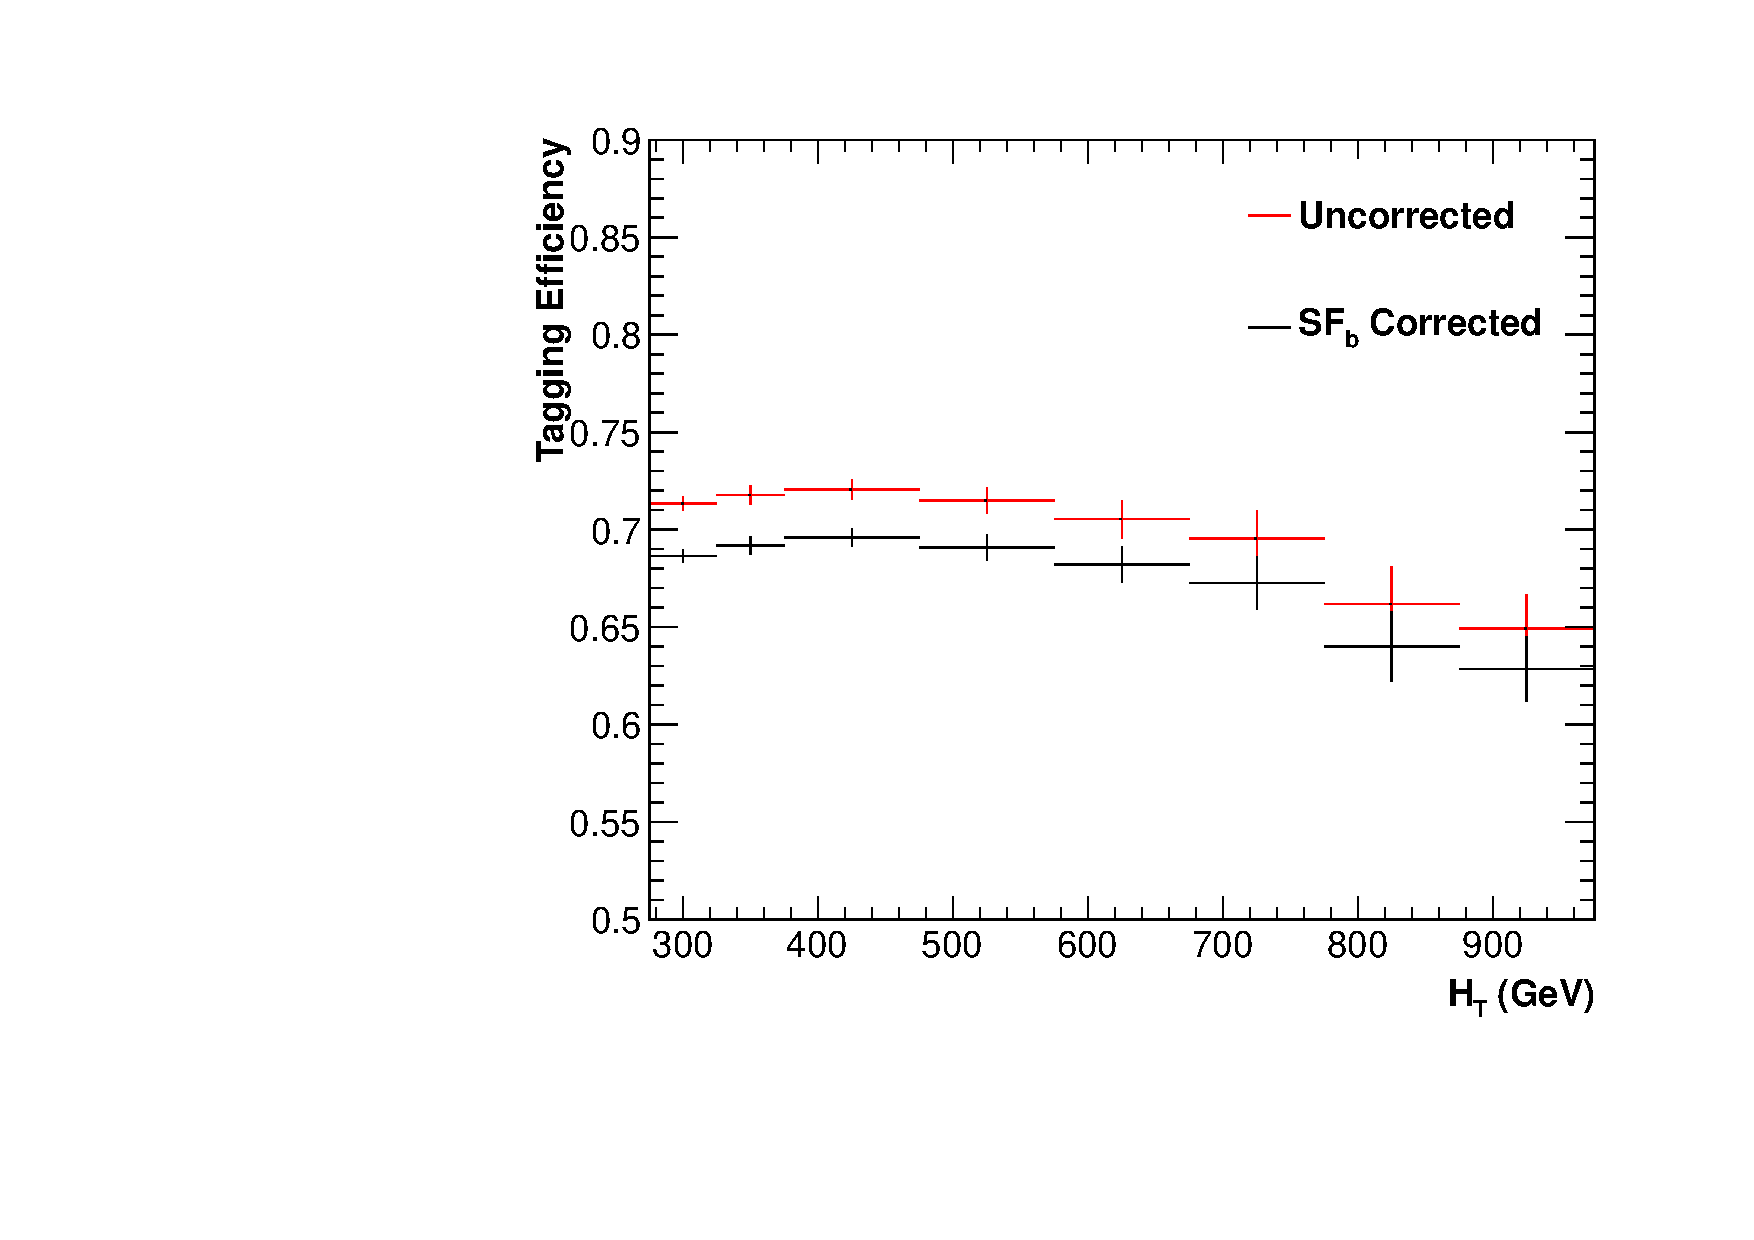
\includegraphics[width = 1.0\linewidth]{plots/b_jet_HTDistribution.pdf}
\centering (a)  b-jets
\end{minipage}
\quad
\begin{minipage}[b]{0.38\linewidth}
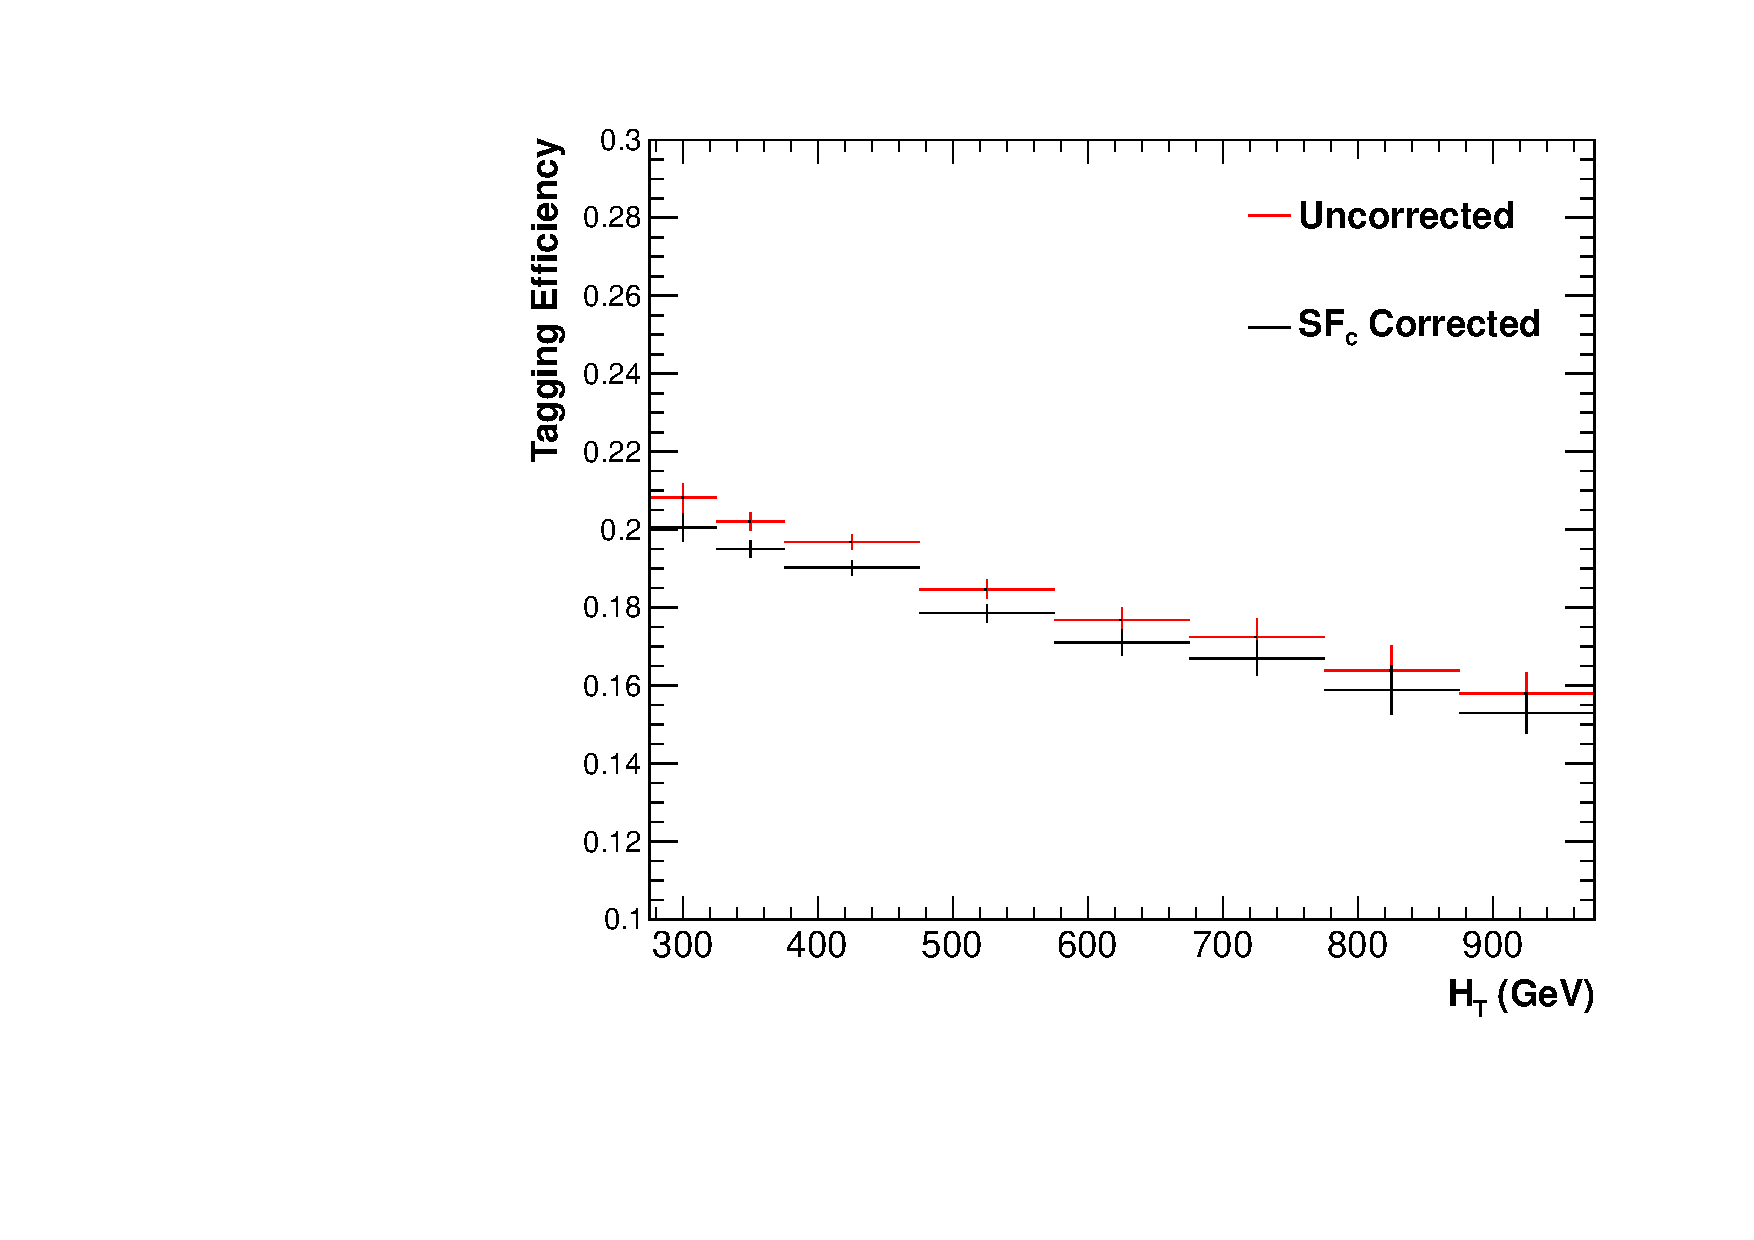
\includegraphics[width = 1.0\linewidth]{plots/c_jet_HTDistribution.pdf}
\centering (b) c-jets
\end{minipage}
\quad
\begin{minipage}[b]{0.38\linewidth}
\centering
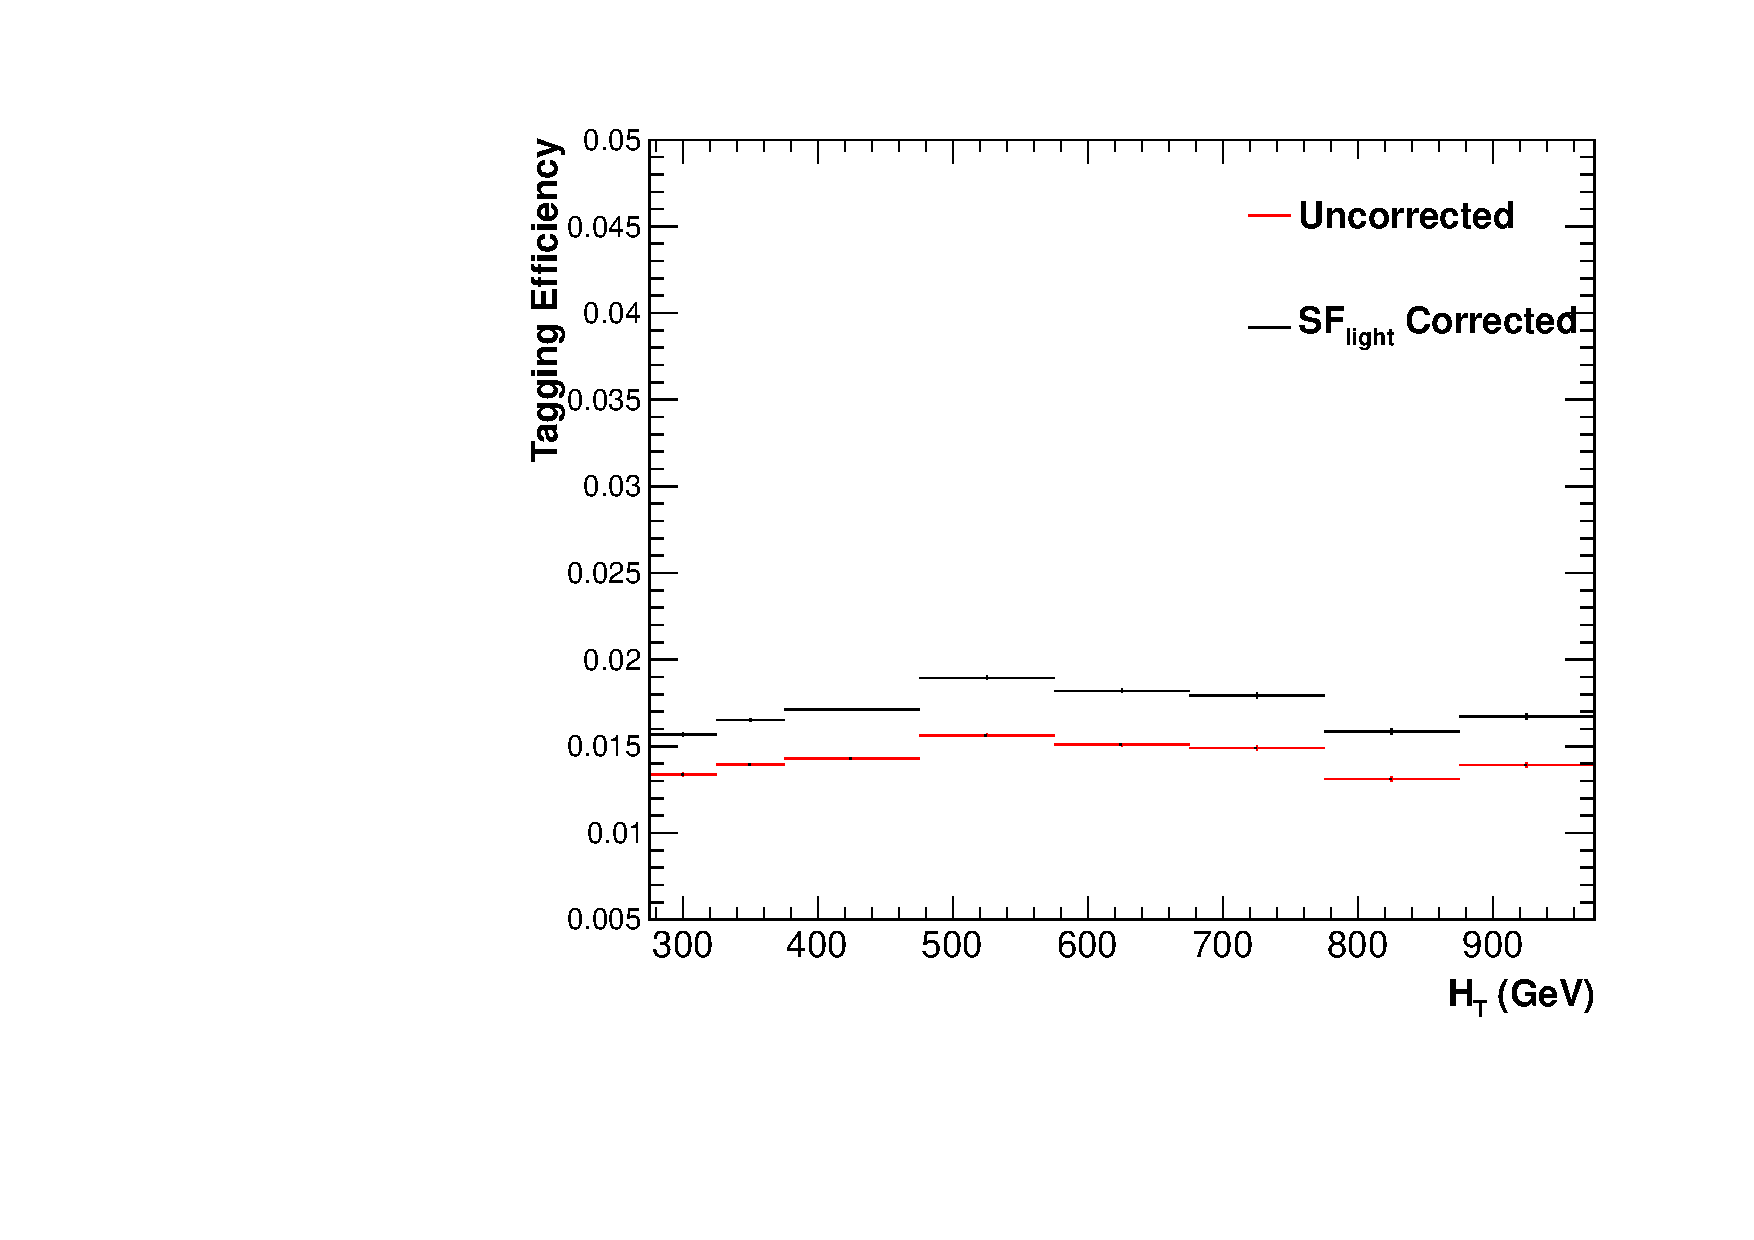
\includegraphics[width = 1.0\linewidth]{plots/light_jet_HTDistribution.pdf}
\centering (c) light-jets
\end{minipage}
\caption[Tagging efficiencies of (a) b-jets, (b) c-jets, and (c$)$ light-jets determined from all jets within each \theht category. ]{Tagging efficiencies of (a) b-jets, (b) c-jets, and (c$)$ light-jets as a function all jets within each \theht category. Efficiencies measured directly from simulation (black) and with data to simulation $SF_{b,c,light}$ correction factors (red) are applied.}\label{fig:btagefficiency}
\end{figure}

\FloatBarrier

Each of the correction factors for the b, c and light flavoured jets come with an associated systematic uncertainty. The uncertainties across different jet \pt and $\eta$ categories, are considered as fully correlated. When computing the magnitude of the effect of this systematic uncertainty on the \ac{TF}s of the analysis, the measured tagging efficiencies for each jet flavour are scaled up/down simultaneously within each \theht and \njet category by the systematic uncertainty of the $SF_{\text{b, c, light}}$ scale factors. 

Varying the scale factor corrections by their systematic uncertainty will change the absolute yields within  each $n_{b}^{reco}$ bin of all selections. However, ultimately it is the change in the \ac{TF}s which influences the final background prediction from each of the control samples. The magnitude of the absolute change in each \ac{TF}, constructed from when the \mupjets control sample is used to predict the entire hadronic signal region background, is shown in Table \ref{tab:btagsfuncertainties}. 

\def\arraystretch{1.3}
\begin{table}[ht!]
\begin{center}
\footnotesize
\begin{tabular*}{0.95\textwidth}{@{\extracolsep{\fill}} ccccc}
\hline
$n_{b}^{reco}$         & 275--325                  & 325--375                  & 375--475                  & 475--575                 \\ 
\hline\hline
\\
= 0                    & 0.557 $^{+0.001}_{-0.001}$  $\pm$  0.012       & 0.495 $^{+0.001}_{-0.001}$  $\pm$  0.009       & 0.383 $^{+0.001}_{-0.001}$  $\pm$  0.005       & 0.307 $^{+0.001}_{-0.002}$  $\pm$  0.006      \\
= 1                    & 0.374 $^{+0.006}_{-0.006}$  $\pm$  0.006       & 0.320 $^{+0.006}_{-0.005}$ $\pm$  0.005        & 0.251 $^{+0.005}_{-0.005}$ $\pm$  0.004        & 0.185 $^{+0.003}_{-0.003}$  $\pm$  0.004      \\
= 2                    & 0.226 $^{+0.002}_{-0.002}$  $\pm$  0.004       & 0.201 $^{+0.001}_{-0.002}$ $\pm$  0.004        & 0.159 $^{+0.001}_{-0.001}$ $\pm$  0.004       & 0.134 $^{+0.000}_{-0.001}$   $\pm$  0.004      \\
= 3                    & 0.221 $^{+0.002}_{-0.002}$  $\pm$  0.005       & 0.208 $^{+0.002}_{-0.001}$ $\pm$  0.007       & 0.164 $^{+0.001}_{-0.000}$  $\pm$  0.006       & 0.144 $^{+0.001}_{-0.001}$   $\pm$  0.007      \\
$\geq$ 4               & 0.222 $^{+0.004}_{-0.005}$  $\pm$  0.015       & 0.248 $^{+0.003}_{-0.003}$ $\pm$  0.035       & 0.123 $^{+0.002}_{-0.003}$  $\pm$  0.009       & -     \\ 
\\
\hline
                       & 575--675                  & 675--775                  & 775--875                  & $\geq$875           \\ 
\hline\hline
\\
= 0                    & 0.263 $^{+0.001}_{-0.002}$  $\pm$  0.006       & 0.215 $^{+0.000}_{-0.001}$  $\pm$  0.007       & 0.171 $_{-0.001}^{+0.000}$ $\pm$  0.009       & 0.111 $_{-0.001}^{+0.000}$  $\pm$  0.006      \\
= 1                    & 0.154 $^{+0.003}_{-0.003}$  $\pm$  0.005       & 0.138 $^{+0.003}_{-0.004}$  $\pm$  0.006       & 0.121 $^{+0.005}_{-0.005}$  $\pm$  0.007       & 0.091 $^{+0.002}_{-0.002}$  $\pm$  0.006      \\
= 2                    & 0.104 $^{+0.000}_{-0.001}$  $\pm$  0.005       & 0.079 $^{+0.001}_{-0.001}$  $\pm$  0.006       & 0.063 $^{+0.001}_{-0.002}$  $\pm$  0.007       & 0.071 $^{+0.000}_{-0.000}$  $\pm$  0.008      \\
= 3                    & 0.116 $^{+0.001}_{-0.001}$  $\pm$  0.009       & 0.069 $^{+0.001}_{-0.001}$  $\pm$  0.007       & 0.079 $^{+0.001}_{-0.001}$  $\pm$  0.017       & 0.095 $_{-0.002}^{+0.003}$  $\pm$  0.020      \\ 

\end{tabular*}
\end{center}
\caption[The absolute change in the \ac{TF}s used to predict the entire signal region \ac{SM} background, using the \mupjets control sample when the systematic uncertainties of the data to simulation scale factors are varied by $\pm 1 \sigma$.]{The absolute change in the \ac{TF}s used to predict the entire signal region \ac{SM} background, using the \mupjets control sample when the systematic uncertainties of the data to simulation scale factors are varied by $\pm 1 \sigma$. The impact of the change is shown for each \theht and $n_{b}^{reco}$ category with no requirement made on the jet multiplicity of the events. (Also quoted are the statistical uncertainties)}\label{tab:btagsfuncertainties}
\end{table}
\def\arraystretch{1.0}

It can be seen that the \ac{TF}s are found to be relatively insensitive to the systematic uncertainty of the b-tag scale factors (showing typically less than $\sim2\%$ change). This can be accounted for by the similar composition of the signal and control sample backgrounds, such that any change in the underlying $n_{b}^{reco}$ distribution will be reflected in both signal and control regions and cancel out in the \ac{TF}. 

Any overall systematic effect on the overall background prediction of the analysis from these b-tag scale factor uncertainties is incorporated within the data driven systematics introduced in the following section.

\section{Systematic Uncertainties on Transfer Factors}
\label{subsec:sysuncertainties}

Since the \ac{TF}s used to establish the background prediction are obtained from simulation, an appropriate systematic uncertainty is assigned to account for theoretical uncertainties \cite{Bern:2011pa} and limitations in the simulation modelling of event kinematics and instrumental effects. 

The magnitudes of these systematic uncertainties are established through a data driven method, in which the three independent control samples of the analysis (\mupjets, \dimupjets, \gpjets) are used to in a series of closure tests. The yields from one of these control samples, along with the corresponding \ac{TF} obtained from simulation, are used to predict the expected yields in another control sample. This procedure therefore utilises the same method used in determining a background prediction for the signal region as already established in Section (\ref{subsec:controlsampledefinition}).

The level of agreement between the predicted and observed yields is expressed as the ratio 

\begin{equation}
\label{eq:closuretests}
\frac{(N_{\text{obs}}-N_{\text{pred}})}{N_{\text{pred}}},
\end{equation}

while considering only the statistical uncertainties on the prediction, $N_{\text{pred}}$,  and the observation, $N_{\text{obs}}$. No systematic uncertainty is assigned to the prediction, and resultantly the level of closure is defined by the statistical significance of a deviation from the ratio from zero.

This ratio is measured for each \theht category in the analysis, allowing these closure tests to be sensitive to both the presence of any significant biases or any possible \theht dependence to the level of closure.

Eight sets of closure tests are defined between the three data control samples, conducted independently between the two jet multiplicity (2 $\leq n_{\text{jet}} \leq 3$, $n_{\text{jet}} \geq 4$ ) categories. Each of these tests are specifically chosen to probe each of the different key ingredients of the simulation modelling that can affect the background prediction.

Each of the different modelling components and the relevant closure tests are described below:

\begin{itemize}

\item[] \textbf{\alphat modelling}

The modelling of the \alphat distribution in genuine \met events is probed with the \mupjets control sample. This test is important to verify the approach of removing the \alphat $>$ 0.55 requirement from the \mupjets and \dimupjets samples to increase the precision of the background prediction. The test uses the \mupjets sample without an \alphat cut to make a prediction into the \mupjets sample defined with the requirement  \alphat $>$ 0.55.

\item[] \textbf{Background admixture}

The sensitivity of the translation factors to the relative admixture of events from $W +$ jets and \ttbar processes is probed by two closure tests. 

Within the \mupjets sample, a W boson enriched sub-sample ($n_{b} =$ 0) is used to predict yields in a \ttbar enriched sub-sample ($n_{b} =$ 1). Similarly, the \ttbar enriched sub-sample ($n_{b} =$1) is also used to predict yields for a further enriched \ttbar sub-sample ($n_{b} =$ 2), further probing the modelling of the \nbreco distribution. 

Similarly a further closure test probes the relative contribution of $Z +$ jets to $W +$jets and \ttbar events, through the use of the \mupjets sample to predict yields for the \dimupjets control sample. This closure test, also at some level probes the muon trigger and reconstruction efficiencies, given that exactly one or two muons are required by the different selections.
 
These tests represent an extremely conservative approach as the admixture of the two backgrounds remains similar when a prediction is made between the control samples and the signal region. This is contrary to the closure tests defined above which make predictions between two very different admixtures of $W +$ jets and \ttbar events.  

\item[] \textbf{Consistency check between \zinv predictions}

This is an important consistency check between the \dimupjets and \gpjets, which are both used in the prediction of the \zinv in the signal region. This is conducted by using the \gpjets sample to predict yields for the \dimupjets control sample. Using \gpjets processes as a method to predict Z + jet processes is subject to theory uncertainties \cite{CMS-PAS-SUS-08-002}, which can be probed by this data driven closure test within a $Z \rightarrow \mu\mu$ control sample. 

\item[]\textbf{Modelling of jet multiplicity}

The simulation modelling of the jet multiplicity within each control sample is important due to the exclusive jet multiplicity categorisation within the analysis. This is probed via the use of each of the three control samples to independently predict from the lower jet multiplicity category $2 \leq n_{\text{jet}} \leq 3$, to the high jet category $n_{\text{jet}} \geq 4$. 

For the case of the \mupjets and \dimupjets control samples, this test also serves as a further probe of the admixture between $W +$ jets/$Z +$ jets and \ttbar. 
\end{itemize}

To test for the assumption that no \theht dependencies exist within the background predictions of the analysis, the first five closure tests defined above are used, with zeroeth and first order polynomial fits applied to each test individually. This is summarised in Table \ref{tab:closuretestfitslow} and Table \ref{tab:closuretestfitshigh} which show the results for both the 2 $\leq n_{jet} \leq 3$ and $\geq 4$ jet multiplicity bins respectively.

 \begin{table}[h!]
 \footnotesize
\begin{center}
\begin{tabular*}{0.95\textwidth}{@{\extracolsep{\fill}}ll|cc|cc}
\cline{1-6}
\multicolumn{2}{c}{} & \multicolumn{2}{c}{Constant fit} & \multicolumn{2}{c}{Linear fit} \\ 
\footnotesize{Closure test} & \multicolumn{1}{c}{Symbol} & \footnotesize{Best fit value} & \multicolumn{1}{c}{p-value} & \footnotesize{Slope (10$^{-4}$)} & \footnotesize{p-value} \\
\hline\hline
\footnotesize{\alphat $< 0.55 \rightarrow \alphat > 0.55$ (\mupjets)} & \footnotesize{Circle} & $-0.06 \pm 0.02$ & 0.93 & $-1.3 \pm 2.2$ & 0.91 \\ 
\footnotesize{0 b-jets $\rightarrow$ 1 b-jet (\mupjets)} & \footnotesize{Square} & $ \footnotesize{\quad}0.07 \pm 0.02$ & 0.98 & $-1.6 \pm 1.6$ & 1.00 \\ 
\footnotesize{1 b-jets $\rightarrow$ 2 b-jet (\mupjets)} & \footnotesize{Triangle} & $ -0.07 \pm 0.03$ & 0.76 & $-2.7 \pm 3.0$ & 0.76 \\ 
\footnotesize{\mupjets $\rightarrow$ \dimupjets} & \footnotesize{Cross} & $ \footnotesize{\quad}0.10 \pm 0.03$ & 0.58 & $-1.1 \pm 2.3$ & 0.49 \\ 
\footnotesize{\dimupjets $\rightarrow$ \gpjets} & \footnotesize{Star} & $ -0.06 \pm 0.04$ & 0.31 & $\footnotesize{\quad}4.2 \pm 4.3$ & 0.29 \\ 
\end{tabular*}
\end{center}
\caption[A summary of the results obtained from zeroeth order polynomial (i.e. a constant) and linear fits to five sets of closure tests performed in the $ 2 \geq n_{\text{jet}} \geq$ 3 category.]{A summary of the results obtained from zeroeth order polynomial (i.e. a constant) and linear fits to five sets of closure tests performed in the $ 2 \geq n_{\text{jet}} \geq$ 3 category.  The two columns show the best fit value for the slope obtained when performing a constant (left) and linear (right) fit and the p-value for that fit.}\label{tab:closuretestfitslow}
\end{table}

 \begin{table}[h!]
\footnotesize
\begin{center}
\begin{tabular*}{0.95\textwidth}{@{\extracolsep{\fill}}ll|cc|cc}
\hline
\multicolumn{2}{c}{} & \multicolumn{2}{c}{\footnotesize{Constant fit}} & \multicolumn{2}{c}{\footnotesize{Linear fit}} \\ 
\footnotesize{Closure test} & \multicolumn{1}{c}{Symbol} & \footnotesize{Best fit value} & \multicolumn{1}{c}{p-value} & \footnotesize{Slope (10$^{-4}$)} & \footnotesize{p-value} \\
\hline\hline
\footnotesize{\alphat $< 0.55 \rightarrow \alphat > 0.55$ (\mupjets)} & \footnotesize{Circle} & $-0.05 \pm 0.03$ & 0.21 &  $\footnotesize{\quad}3.0 \pm 2.9$ & 0.21 \\ 
\footnotesize{0 b-jets $\rightarrow$ 1 b-jet (\mupjets)} & \footnotesize{Square} & $ -0.03 \pm 0.03$ & 0.55 & $-1.0 \pm 1.9$ & 0.47 \\ 
\footnotesize{1 b-jets $\rightarrow$ 2 b-jet (\mupjets)} & \footnotesize{Triangle} & $ -0.02 \pm 0.03$ & 0.39 & $ \footnotesize{\quad}1.1 \pm 2.2$ & 0.31 \\ 
\footnotesize{\mupjets $\rightarrow$ \dimupjets} & \footnotesize{Cross} & $  \footnotesize{\quad}0.08 \pm 0.07$ & 0.08 &  $\footnotesize{\quad}4.8 \pm 4.3$ & 0.07 \\ 
\footnotesize{\dimupjets $\rightarrow$ \gpjets} & \footnotesize{Star} & $ -0.03 \pm 0.10$ & 0.72 & $-4.0 \pm 7.0$ & 0.64 \\ 
\end{tabular*}
\end{center}
\caption[A summary of the results obtained from zeroeth order polynomial (i.e. a constant) and linear fits to five sets of closure tests performed in the $n_{\text{jet}} \geq$ 4 category.]{A summary of the results obtained from zeroeth order polynomial (i.e. a constant) and linear fits to five sets of closure tests performed in the $n_{\text{jet}} \geq$ 4 category. The two columns show the best fit value for the slope obtained when performing a constant (left) and linear (right) fit and the p-value for that fit.}\label{tab:closuretestfitshigh}
\end{table}

Table \ref{tab:closuretestfitsall} shows the same fits applied to the three closure tests that probe the modelling between the two $n_{\text{jet}}$ categories. The best fit value and its uncertainty is listed for each set of closure tests in all three tables, along with the p-value of the constant and linear fits applied. 

 \begin{table}[h!]
 \footnotesize
\begin{center}
\begin{tabular*}{0.95\textwidth}{@{\extracolsep{\fill}}ll|cc|cc}
\hline
\multicolumn{2}{c}{} & \multicolumn{2}{c}{\footnotesize{Constant fit}} & \multicolumn{2}{c}{\footnotesize{Linear fit}} \\ 
\footnotesize{Closure test} & \multicolumn{1}{c}{Symbol} & \footnotesize{Best fit value} & \multicolumn{1}{c}{p-value} & \footnotesize{Slope (10$^{-4}$)} & \footnotesize{p-value} \\
\hline\hline
\footnotesize{\mupjets} & \footnotesize{Inverted triangle} & $-0.03 \pm 0.02$ & 0.02 & $\footnotesize{\quad}0.0 \pm 1.0$ & 0.01 \\ 
\footnotesize{\mupjets (outlier removed)} & \footnotesize{Inverted triangle} & $-0.04 \pm 0.01$ & 0.42 & $-1.4 \pm 1.1$ & 0.49 \\ 
\footnotesize{\gpjets} & \footnotesize{Diamond} & $  \footnotesize{\quad}0.12 \pm 0.05$ & 0.79 & $\footnotesize{\quad}6.0 \pm 4.7$ & 0.94 \\ 
\footnotesize{\dimupjets} & \footnotesize{Asterisk} & $ -0.04 \pm 0.07$ & 0.20 &  $\footnotesize{\quad}4.9 \pm 4.4$ & 0.20 \\ 
\end{tabular*}
\end{center}
\caption[A summary of the results obtained from zeroeth order polynomial (i.e. a constant) and linear fits to three sets of closure tests performed between the 2 $\leq$ $n_{\text{jet}}$ $\leq$ 3 and $n_{\text{jet}} \geq$ 4 categories.]{A summary of the results obtained from zeroeth order polynomial (i.e. a constant) and linear fits to three sets of closure tests performed between the 2 $\leq$ $n_{\text{jet}}$ $\leq$ 3 and $n_{\text{jet}} \geq$ 4 categories.  The two columns show the best fit value for the slope obtained when performing a constant (left) and linear (right) fit and the p-value for that fit.}\label{tab:closuretestfitsall}
\end{table}

The best fit value for the constant parameter is indicative of the level of closure, averaged across the full \theht range of the analysis, and the p-value an indicator of any significant dependence on \theht within the closure tests. The best fit values of all the tests are either statistically compatible with zero bias (i.e. less than $2\sigma$ from zero) or at the level of 10\% or less, with the exception of one closure test discussed below. 

Within Table \ref{tab:closuretestfitsall}, there exists one test that does not satisfy the above statement, which is the $2 \leq n_{jet} \leq 3 \rightarrow n_{jet} \geq 4$ test using the \mupjets control sample. The low p-value can be largely attributed to an outlier between 675 $<$ \theht $<$ 775 \GeV, rather than any significant trend in \theht. Removing this single outlier from the constant fit performed, gives a best fit value of $-0.04 \pm 0.01$, $\chi^{2} /$ d.o.f = 6.07/6. and a p-value of 0.42. These modified fit results are also included in Table \ref{tab:closuretestfitsall}.

Additionally, it is found that the best fit values for the slope terms of the linear fits in all three tables are of the order $10^{-4}$, which corresponds to a percent level change per 100 \GeV. However in all cases, the best fit values are fully compatible with zero (within 1$\sigma$) once again with the exception detailed above, indicating that the level of closure is indeed \theht independent.

\subsection{Determining Systematic Uncertainties from Closure Tests}
\label{subsec:determinesystematics}

Once it has been established that no significant bias or trend exists within the closure tests, systematic uncertainties are determined. The statistical precision of the closure tests is considered a suitable benchmark for determining the systematic uncertainties that are assigned to the \ac{TF}s, which are propagated through to the likelihood fit.

The systematic uncertainty band is split into five separate regions of \theht. Within each region the square root of the sample variance, $\sigma^{2}$, is taken over the eight closure tests to determine the systematic uncertainties to be applied within that region.

Using this procedure the systematic uncertainties for each region are calculated and are shown in Table \ref{tab:sysuncert}, with the systematic uncertainty to be used in the likelihood model conservatively rounded up to the nearest decile and applied across all \nbreco categories.

 \begin{table}[h!]
 \footnotesize
\begin{center}
\begin{tabular*}{0.95\textwidth}{@{\extracolsep{\fill}}lcc}
\cline{1-3}
\theht band (\GeV)& $2 \leq n_{jet} \leq 3$ & $n_{jet} \geq 4$ \\
\hline\hline
275 $<$ \theht $<$ 325 & 10\% & 10\% \\
325 $<$ \theht $<$ 375& 10\%  & 10\% \\
375 $<$ \theht $<$ 575& 10\%  & 10\% \\
575 $<$ \theht $<$ 775& 20\%  & 20\% \\
\theht $>$ 775& 20\%  & 30\% \\
\end{tabular*}
\end{center}
\caption[Calculated systematic uncertainties for the five \theht regions, determined from the closure tests. ]{Calculated systematic uncertainties for the five \theht regions, determined from the closure tests. Uncertainties shown for both jet multiplicity categories. Values used within the likelihood model are conservatively rounded up to the nearest decile.}\label{tab:sysuncert}
\end{table}

Figure \ref{fig:uncertaintyplots} shows the sets of closure tests overlaid on top of grey bands that represent the \theht dependent systematic uncertainties. These systematic uncertainties are assumed to be fully uncorrelated between the different $n_{b}$ multiplicity categories and across the five \theht regions. This can be considered a more conservative approach given that some correlations between adjacent \theht categories could be expected due to comparable kinematics.

\begin{figure}[ht]
\centering
\begin{minipage}[b]{0.85 \linewidth}
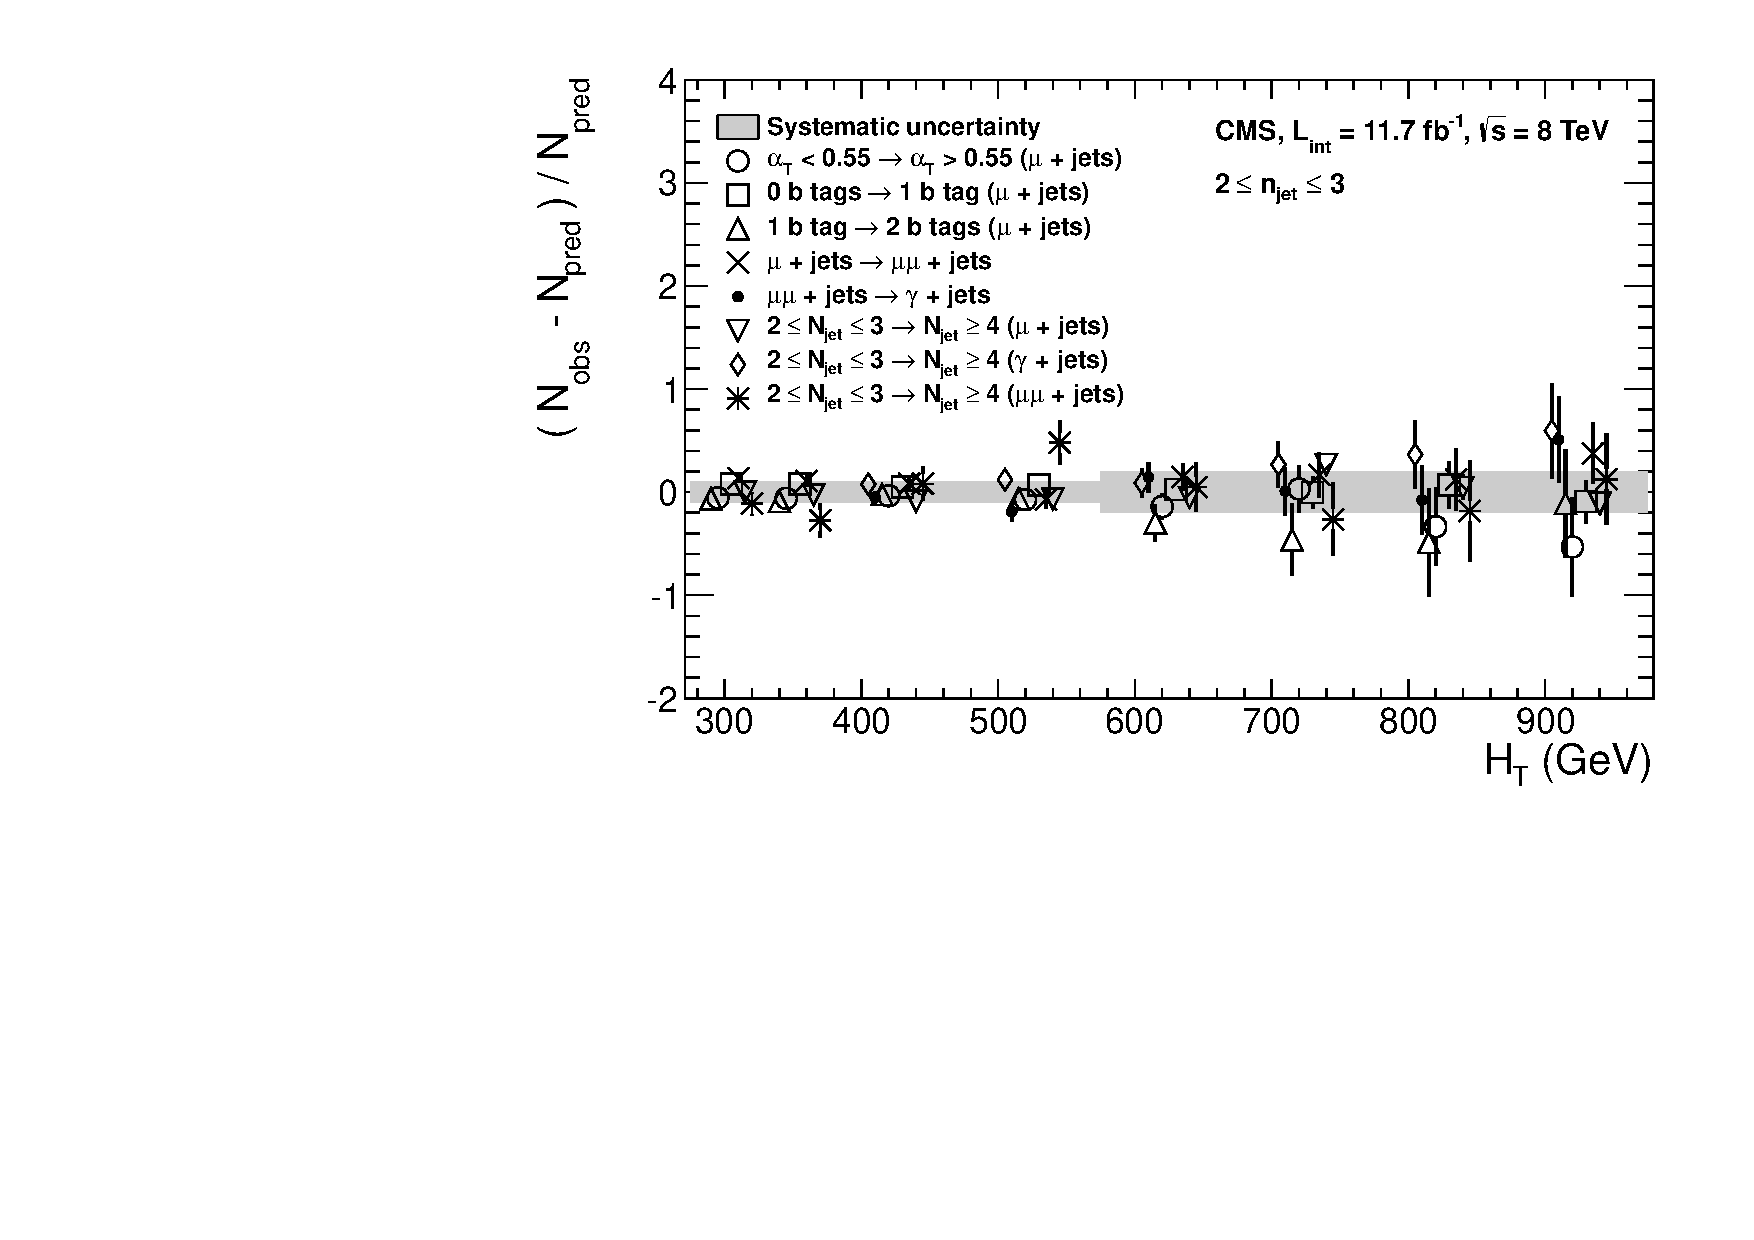
\includegraphics[width = 1.0\linewidth]{plots/syst-le3j.pdf}
\centering(a)  
\end{minipage}
\quad
\begin{minipage}[b]{0.85\linewidth}
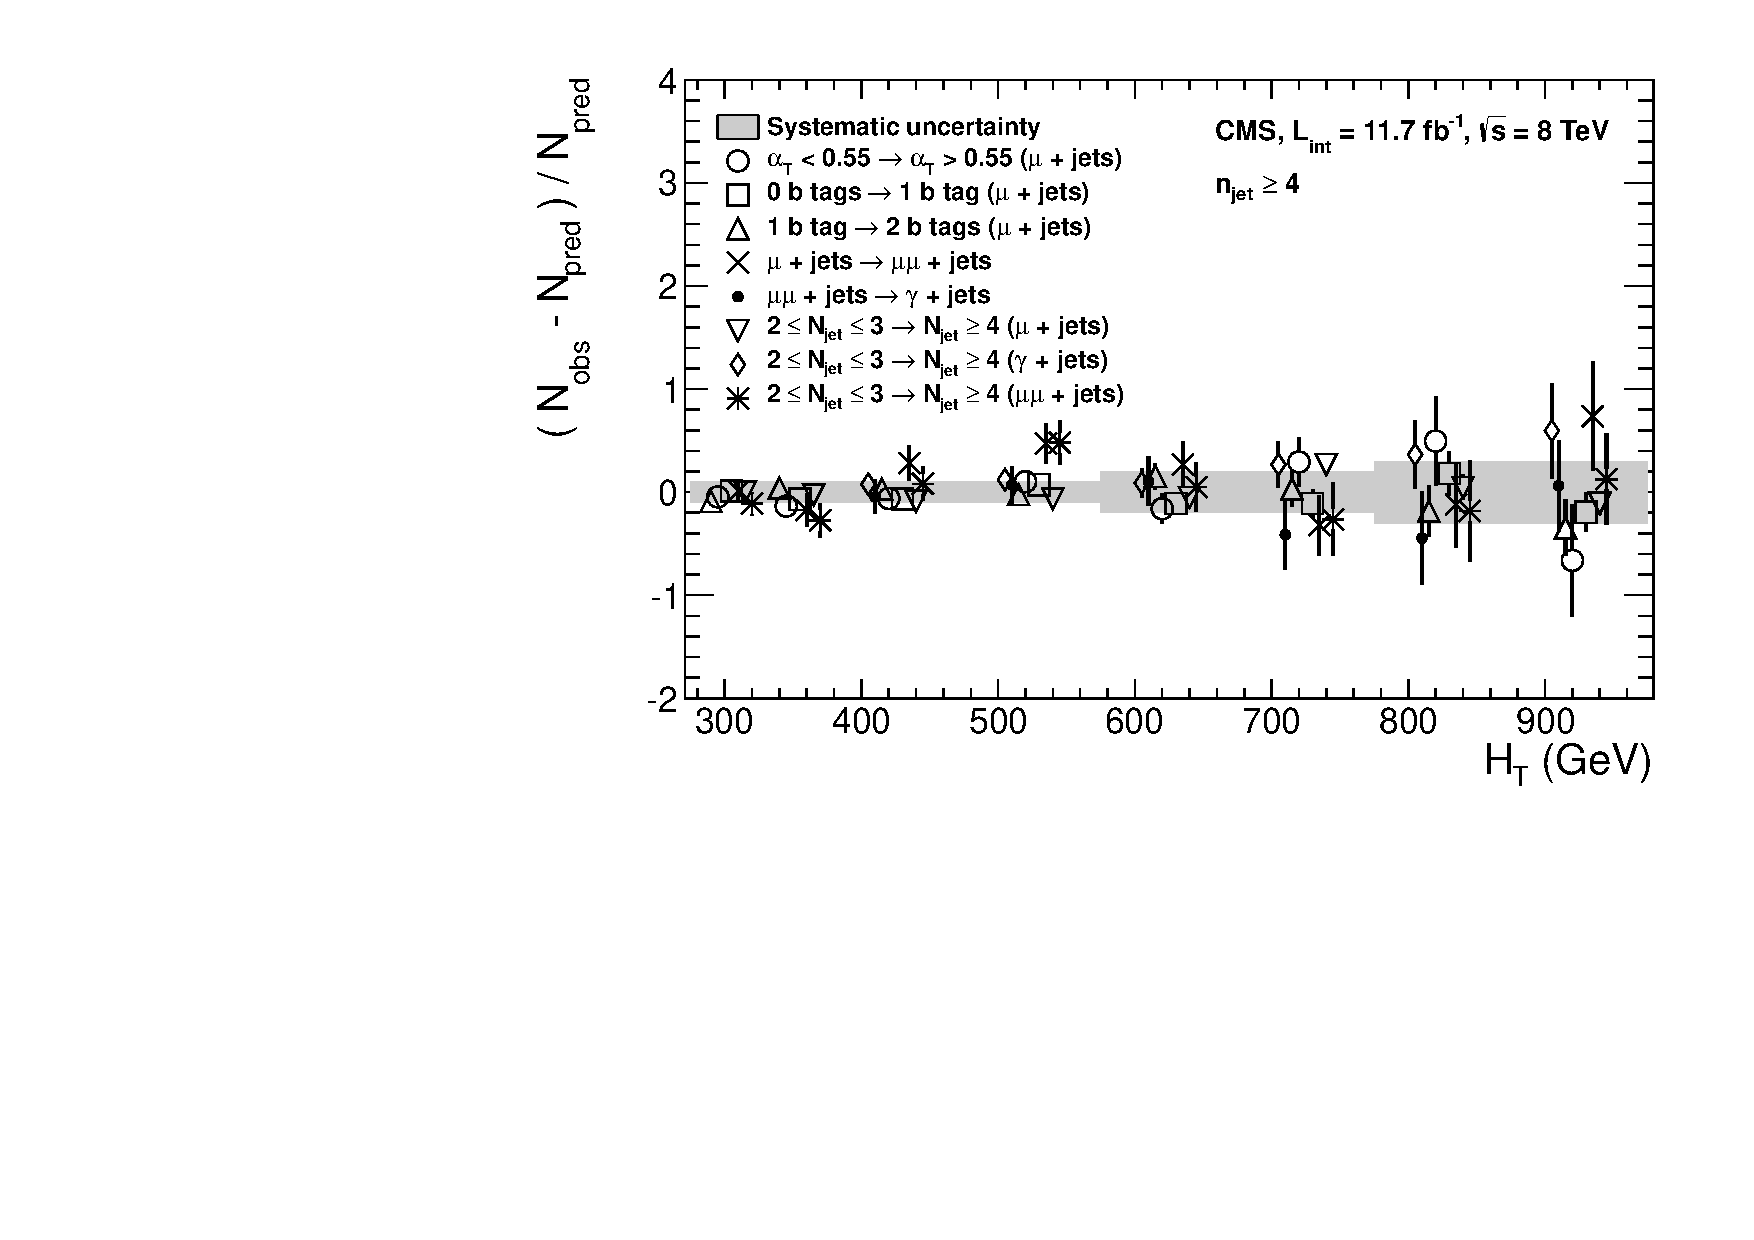
\includegraphics[width = 1.0\linewidth]{plots/syst-ge4j.pdf}
\centering(b) 
\end{minipage}
\caption[Sets of closure tests overlaid on top of the systematic uncertainty used for each of the five \theht regions.]{Sets of closure tests (open symbols) overlaid on top of the systematic uncertainty used for each of the five \theht regions (shaded bands) and for the two different jet multiplicity categories: (a) $2 \leq n_{\text{jet}} \leq 3$ and (b) $n_{\text{jet}} \geq 4$.}
\label{fig:uncertaintyplots}
\end{figure}

These closure tests represent a conservative estimate of the systematic uncertainty in making a background prediction for the signal region. This is due to significant differences in the background composition and event kinematics between the two sub-samples used in the closure tests. This is not the case when a signal region prediction is made, due to the two sub-samples both having a comparable background admixture and similar kinematics owing to the fact that the \ac{TF}s are always constructed using the same ($n_{\text{jet}}$, \nbreco, \theht) category.

This point is emphasised when we examine the sensitivity of the \ac{TF}s to a change in the admixture of W + jets and \ttbar with the control and signal samples. This is accomplished by varying the cross-sections of the W +jets and \ttbar by +20\% and -20\%, respectively. Figures \ref{fig:xsecvariedle3j} and \ref{fig:xsecvariedge4j} within Appendix \ref{app:backgroundestimation}, show the effect upon the closure tests for both jet multiplicity categories. Given these variations in cross-sections, the level of closure is found to be significantly worse, with biases as large as $\sim$ 30\%, most apparent in the lowest \theht bins. However, the \ac{TF}s used to extrapolate from control to signal are seen to change only at the percent level by this large change in cross-section, shown in Table \ref{tab:xsecvaried}.

Given the robust behaviour of the translation factors with respect to large (and opposite) variations in the W + jets and \ttbar cross-sections, one can assume with confidence that any bias in the translation factors is adequately (and conservatively) covered by the systematic uncertainties used in the analysis.

\section{Simplified Models, Efficiencies and Systematic Uncertainties}
\label{sec:smsmodels}

The results of the analysis are interpreted using various \ac{SMS} signal models, which as already introduced in Section (\ref{subsec:sms}) offer a natural starting point for quantifying and characterising \ac{SUSY} signals, and a means to identify the boundaries of search sensitivity for different mass splittings, kinematic ranges, and final states. 

Each model is parameterised in a two dimensional parameter space, ($m_{\widetilde{q}/\widetilde{g}}$, $m_{\text{LSP}}$), from which upper limits on the production cross-sections of the various \ac{SMS} models can be set.

Each signal sample is generated at \acf{LO} with Pythia \cite{Sjostrand:2006za}, and cross-sections calculated for \acf{NLO} and \acf{NLL} \cite{Beenakker:1996ch}, with events simulated using the \texttt{Fastsim} framework. This framework represents a simplified simulation of the \ac{CMS} detector, but allows for faster production of various signal topologies with different mass parameters. 

A series of correction factors are applied to account for differences between \texttt{Fastsim} \cite{1742-6596-331-3-032049} and \texttt{Fullsim} \cite{1742-6596-331-3-032015} simulation, which can affect the resultant \nbreco distribution and which are detailed in Section (\ref{subsec:smsbtagreweighting}). 

\subsection{Signal Efficiency}

The analysis selection efficiency, \epsilon, is measured for each mass point of the interpreted model. This serves as a measure of the sensitivity of the signal selection for that particular sparticle, \ac{LSP} mass and final state topology. The signal yield is then given by

\begin{equation}
Y(m_{\widetilde{q}/\widetilde{g}},m_{LSP}) = \epsilon \times \sigma \times \mathcal{L},
\end{equation}

where $\sigma$ represents the model's cross-section and $\mathcal{L}$ the luminosity. An upper limit on \sigma taken from theory can then allow for the setting of limits in terms of the particle mass. 

Figure \ref{fig:smsefficiencyplots} shows the expected signal efficiency of the signal selection for the \texttt{T1} and \texttt{T2} \ac{SMS} models interpreted in this analysis. The efficiency maps are produced with the requirement $\theht >$ 275 \GeV (i.e. no \theht categorisation) and requirements on $n_{\text{jet}}$ and $n_{b}^{reco}$ are the most sensitive to the model in question.


\begin{figure}[ht]
\centering
\begin{minipage}[b]{0.45 \linewidth}
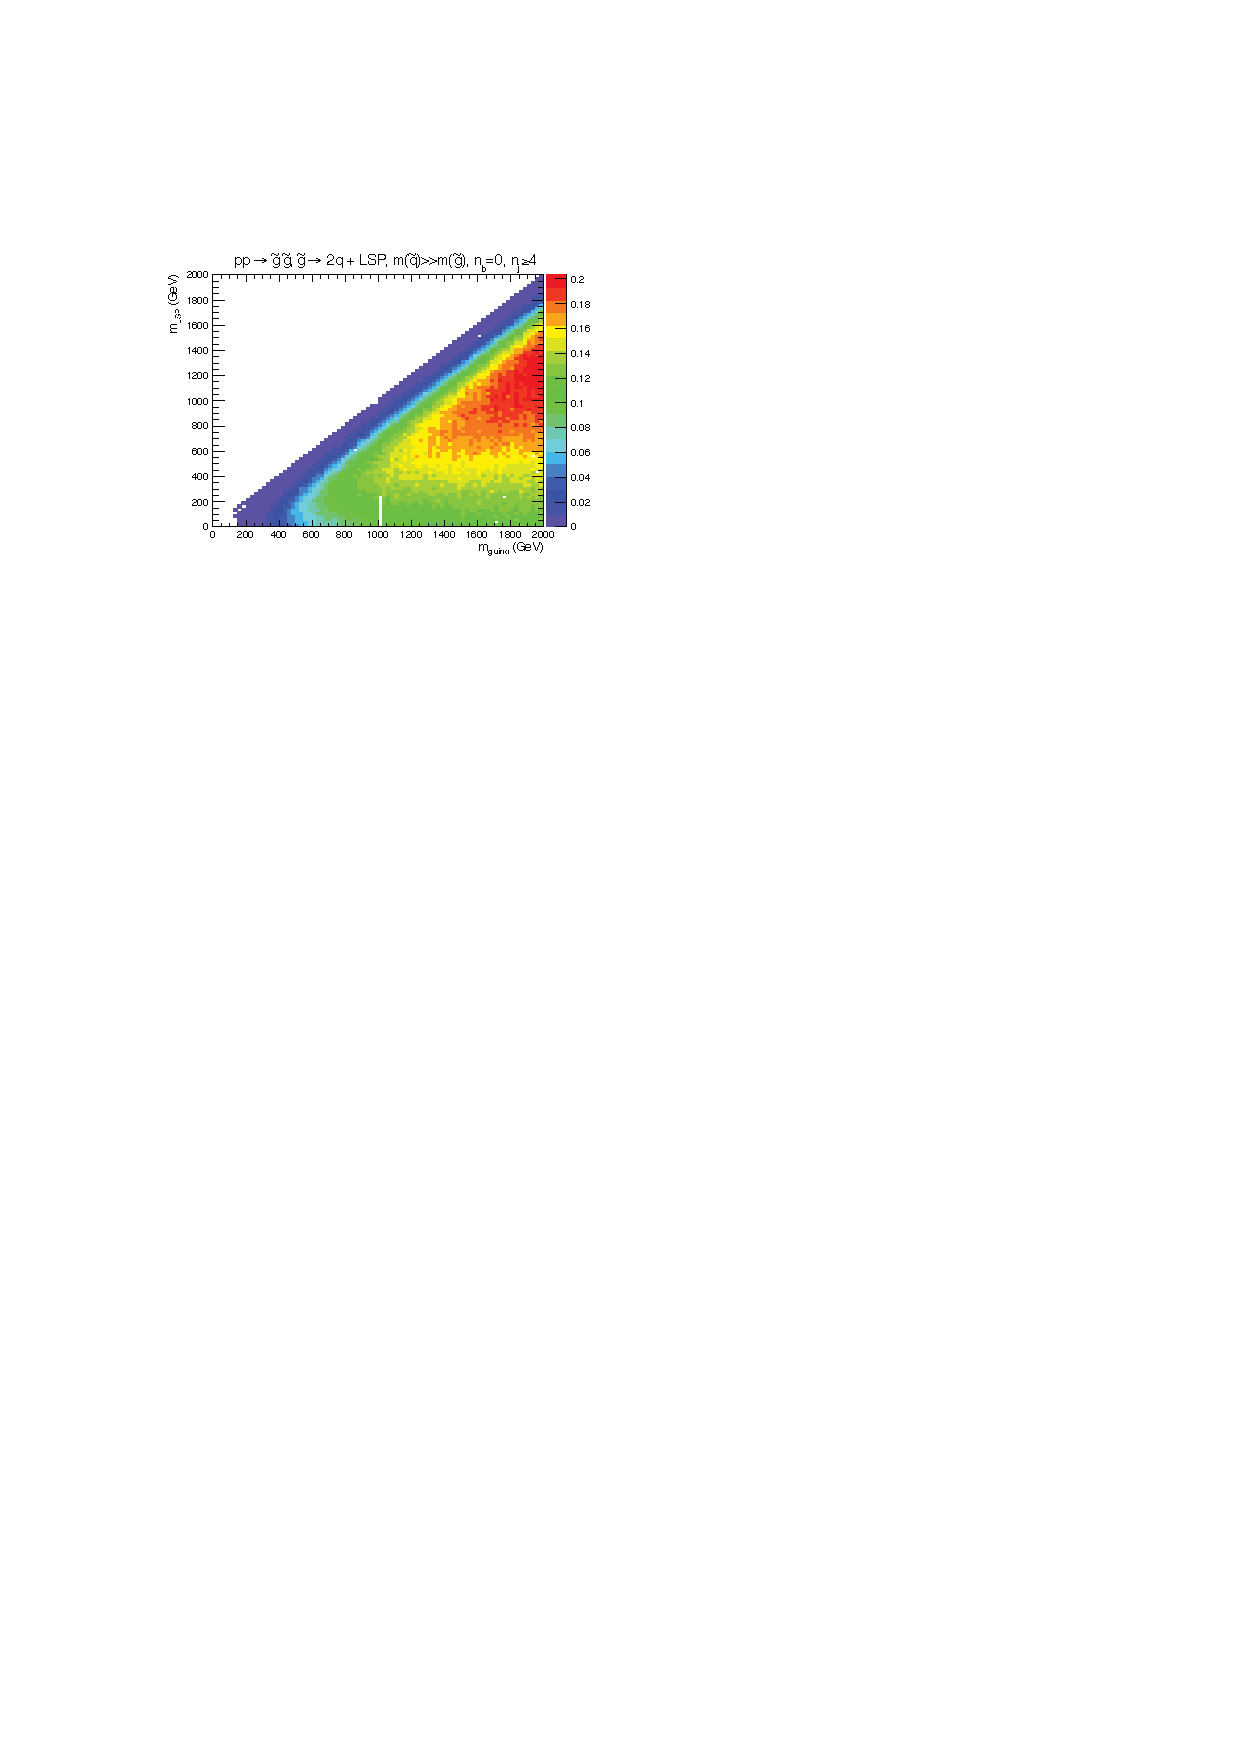
\includegraphics[width = 1.0\linewidth]{plots/t1_signal_eff.pdf}
\centering(a) Model \texttt{T1}, $n_{jet} \geq 4$, $n_{b}^{reco} = 0$ 
\end{minipage}
\quad
\begin{minipage}[b]{0.45\linewidth}
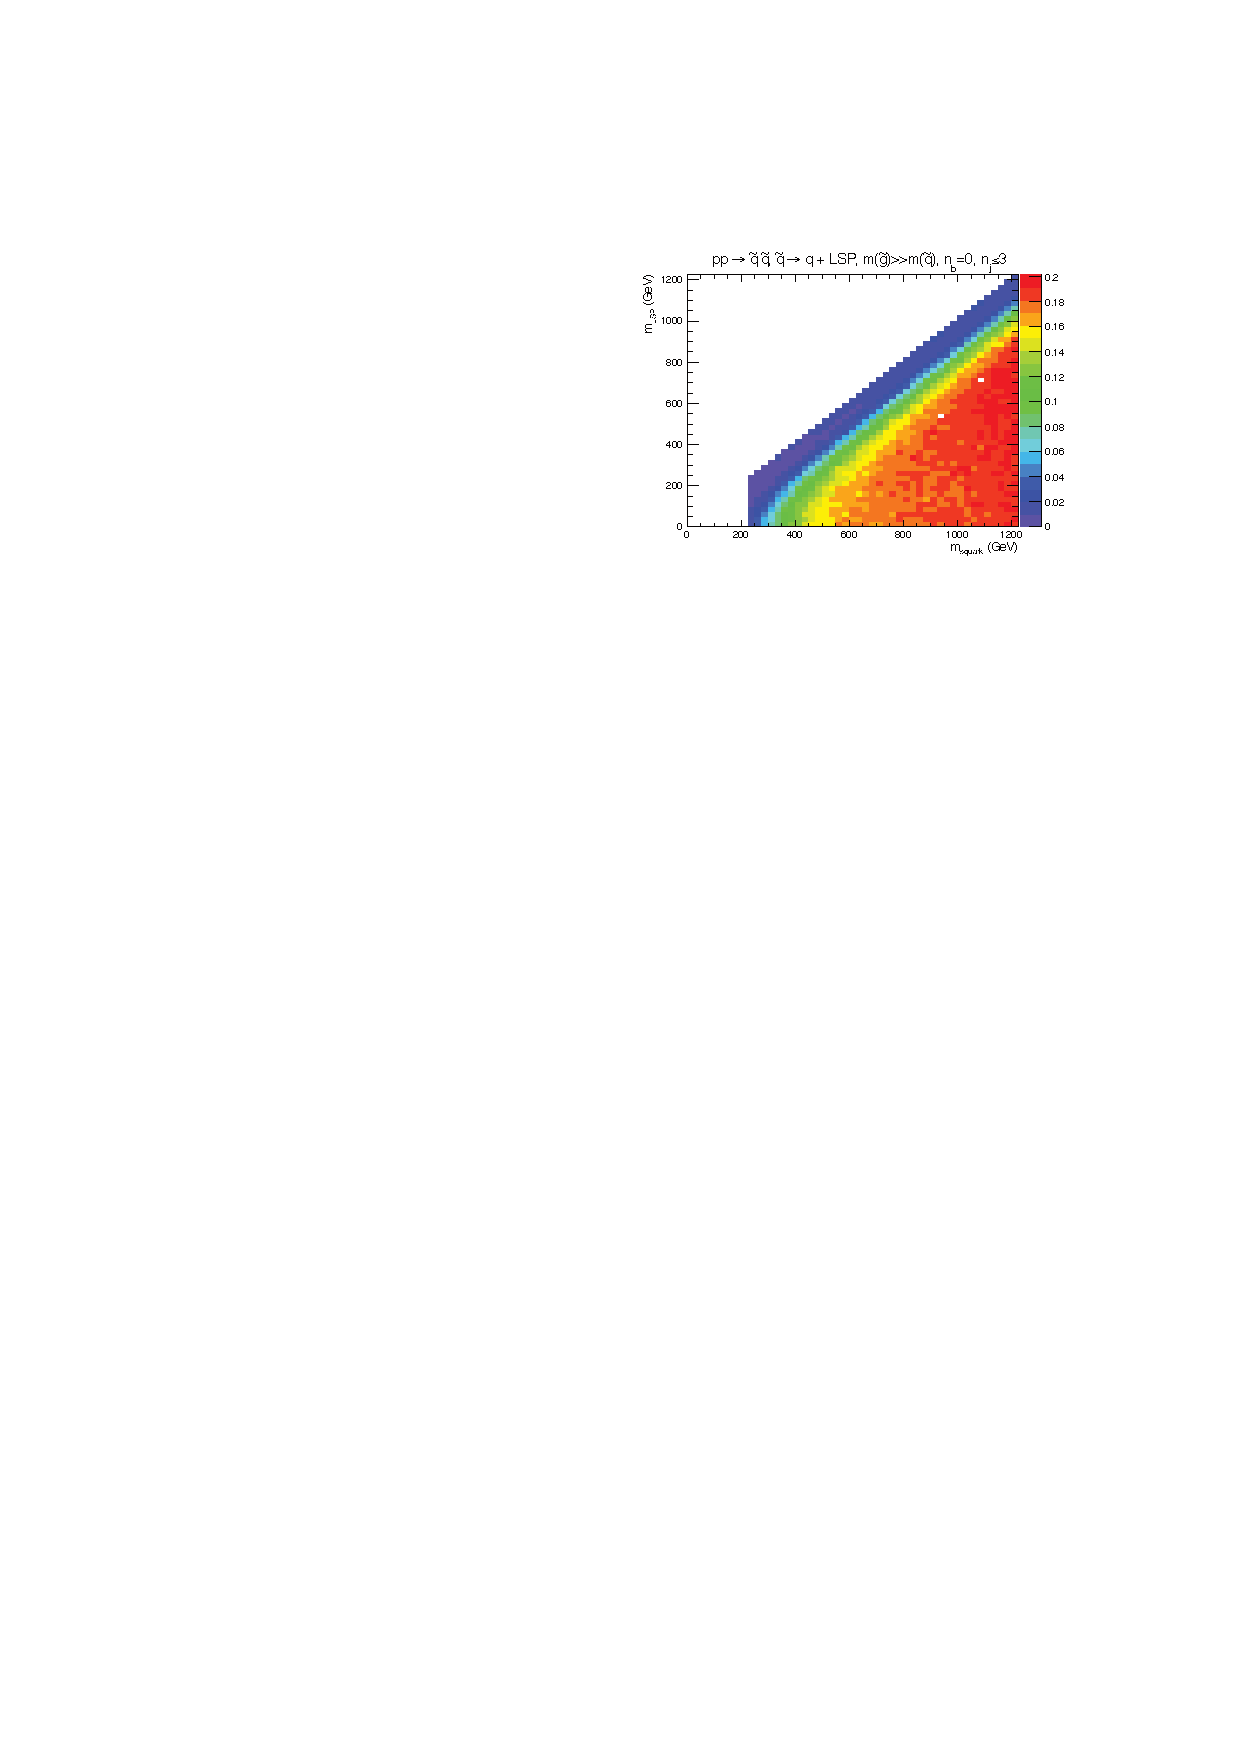
\includegraphics[width = 1.0\linewidth]{plots/t2_signal_eff.pdf}
\centering(b)  Model \texttt{T2}, $n_{jet} \leq 3$, $n_{b}^{reco} = 0$ 
\end{minipage}
\caption[Signal efficiencies fo the \ac{SMS} models (a) \texttt{T1} and (b) \texttt{T2}.]{Signal efficiencies for the \ac{SMS} models (a) \texttt{T1} ($\widetilde{g}\widetilde{g}^{*}\rightarrow q\bar{q}\widetilde{\chi}^{0}_{1}q\bar{q}\widetilde{\chi}^{0}_{1}$) and (b) \texttt{T2} ($ \widetilde{q}\widetilde{q}^{*} \rightarrow q\widetilde{\chi}^{0}_{1}\bar{q}\widetilde{\chi}^{0}_{1}$) when requiring $n_{jet} \geq 4$ and $\leq 3$ respectively, and $n_{b}^{reco} = 0$.}
\label{fig:smsefficiencyplots}
\end{figure}


The same procedure is conducted in the analysis control samples. It is found in the \mupjets control samples, that the signal-to-background ratios for the expected signal yields in each of the \ac{SMS} models are many times smaller than in the hadronic signal region. The relative contamination for the \dimupjets sample is smaller still due to the requirement of a second muon. The relative contamination for the \gpjets sample is expected to be zero for the models under consideration. These small, relative levels of contamination are accounted for in the fitting procedure, as described in Section (\ref{subsec:signalcontribution}).


\subsection{Applying B-tagging Scale Factor Corrections in Signal Samples}
\label{subsec:smsbtagreweighting}

High-statistic \texttt{FastSim} signal simulation samples are unavailable for each signal point, which means that a different procedure to the formula method described in Section (\ref{subsec:backgroundestimation}) is employed. Furthermore, the use of the \texttt{FastSim} framework in the reconstruction introduces an extra set of scale-factor corrections, to be applied simultaneously with those correcting \texttt{FullSim} to the data. 

For these signal models, an event-by-event re-weighting procedure is applied. This applied weight depends on both the flavour content and the b-tagging status of the reconstruction level jets in the event. 

The re-weighting procedure can be described by first considering a single jet within a signal event. The flavour of the jet is determined using the method described in Section (\ref{subsec:formulamethod}). 

Maps of the tagging efficiencies, parameterised as a function of jet \pt and \eta are produced from \texttt{FullSim} simulation samples for each of the b, c and light jet flavours. These efficiencies are calculated from simulation events which pass the hadronic signal selection. The \pt and \eta binning of each map is chosen to match the correction maps of \texttt{FullSim} to data defined in \cite{btagscalefactor}. 

The actual tagging efficiency of the \texttt{FastSim} jet, $\epsilon_{\texttt{FastSim}}(\pt,\eta,f)$, differs from that measured in \texttt{FullSim},  $\epsilon_{MC}(\pt,\eta,f)$, as detailed above and is related via an additional correction factor,

\begin{equation}
\epsilon_{\texttt{FastSim}}(\pt,\eta,f) =  \frac{\epsilon_{MC}(\pt,\eta,f)}{SF_{\texttt{Fast}\rightarrow\texttt{Full}}(\pt,\eta,f)}.
\end{equation}

$SF_{\texttt{Fast}\rightarrow\texttt{Full}}(\pt,\eta,f)$ represents a set of \pt and \eta dependant corrections, that are specific for each \ac{SMS} model. These corrections are calculated from the ratio of tagging rates between a \texttt{FullSim} \ttbar sample, and a selection of mass points from each \texttt{FastSim} \ac{SMS} model, again measured individually for b, c and light-flavoured jets. 

The tagging efficiencies measured in data \cite{btagscalefactor}, $\epsilon_{Data}(\pt,\eta,f)$,  can then be related to $\epsilon_{\texttt{FastSim}}(\pt,\eta,f)$ by the equation,

\begin{align}
\epsilon_{Data}(\pt,\eta,f) &=  \epsilon_{MC}(\pt,\eta,f) \times SF_{MC\rightarrow Data}(\pt,\eta,f) \nonumber \\
&=  \epsilon_{\texttt{FastSim}}(\pt,\eta,f) \times \underbrace{SF_{\texttt{Fast}\rightarrow\texttt{Full}}(\pt,\eta,f) \times SF_{MC\rightarrow Data}(\pt,\eta,f)}_\text{SF$_{\texttt{Fast}} \rightarrow Data$}.
\end{align}

For each jet, the weight of the event is re-weighted according to whether the jet fires the tagger. In the instance that the jet \emph{is} tagged, the event weight will be modified by,

\begin{equation}
\text{weight} = SF_{\texttt{Fast} \rightarrow Data} \times \text{weight},
\end{equation} 
and in the case that the jet does \emph{not} fire the tagger,

\begin{equation}
\text{weight} = \frac{1-\epsilon_{Data}(\pt,\eta,f)}{1- \epsilon_{\texttt{FastSim}}(\pt,\eta,f)}\times \text{weight}.
\end{equation}

This procedure is applied to all events that pass the selection criteria, thus correcting the \texttt{FastSim} \nbreco distribution to data. 

\subsection{Experimental Uncertainties}

The systematic uncertainty on the expected signal acceptance $\times$ analysis efficiency is determined independently for the each \ac{SMS} model considered. These systematics stem from uncertainties on the parton distribution functions, the luminosity measurement, jet energy scale, b-tag scale factor measurements and the efficiencies of various selection criteria used in the signal selection, including the \mht / \met, dead \ac{ECAL} cleaning filter and lepton / photon event vetoes. 

Rather than trying to estimate the level of systematic that is applicable point-by-point in a model space, general behaviours are considered; and instead constant systematics are estimated in two regions of the \ac{SMS} models parameter space. 

These two regions are defined as, near (small mass splittings) and far (large mass splittings) from the mass degenerate diagonal, where the far region is bounded by the condition

\begin{equation}
m_{\widetilde{q}/\widetilde{g}} - m_{LSP} > 350 \GeV \quad && m_{\widetilde{q}/\widetilde{g}} > 475 \GeV. \nonumber
\end{equation}

The total systematics in each region are evaluated in the following ways:

\begin{itemize}
\item[]\textbf{Jet energy scale:} 
The relative change in the signal efficiency is gauged by varying the energy of all jets in an event up or down according to a \pt and \eta dependent jet energy scale uncertainty. Within the two systematic regions, the resulting systematic uncertainties for each \ac{SMS} model are determined by taking the value of the 68$^{\text{th}}$ percentile for the distributions of the relative change in the signal efficiency.
\item[]\textbf{Luminosity measurement:} 
The uncertainty on the measurement of the luminosity collected propagates through to an uncertainty on the signal event yield when considering any new physics model, which is currently 4.4\% \cite{CMS-PAS-LUM-12-001}.
\item[]\textbf{Parton density function} :
Each signal sample is produced using the CTEQ6L1 parton density function. The effect on the signal acceptance when re-weighting to the central value of three different parton distribution functions, CT10, MSTW08 and NNPDF2.1 are examined \cite{Botje:2011sn}. It is found that the change of the signal efficiency in different \ac{SMS} models, due to the alternate PDF sets are typically a few percent, and approaches 10\% at higher squark/gluon and \ac{LSP} masses.
\item[]\textbf{\mht/\met cleaning filter:} 
The ratio of the efficiencies of the cleaning filter are compared in simulation and data after application of the \mupjets control sample selection. No \alphat requirement or further event cleaning filters are applied. The ratio of the efficiencies observed in data and simulation for a cut value of \mht/\met $<$ 1.25 and the two jet multiplicity categories, $2 \leq n_{\text{jet}} \leq 3$ and $n_{\text{jet}} \geq 4$ are 1.028 $\pm$ 0.007 and 1.038 $\pm$ 0.015 respectively. These deviations are taken to represent the systematic uncertainty on the simulation modelling of this variable.
\item[]\textbf{Dead ECAL cleaning filter:} 
The ratio of the efficiencies observed in data and simulation for this filter in the two jet multiplicity categories, $2 \leq \njet \leq 3$ and $\njet \geq 4$, are 0.961 $\pm$ 0.008 and 0.961 $\pm$ 0.009, respectively. These deviations from unity are taken to represent the systematic uncertainties in the modelling in simulation of this filter.
\item[]\textbf{Lepton and photon vetoes:} 
The uncertainty on the efficiency of the lepton and photon vetoes is determined by considering truth information. The efficiency of the vetoes is measured after applying relevant object filters with identical logic, but based on truth instead of reconstructed objects. Where the efficiency is found to not be 100\%, it is taken to represent the fraction of signal events that are incorrectly vetoed. This deviation is taken directly as the systematic uncertainty on the efficiency. The systematic uncertainty is only non-zero for models which contain third-generation quarks in the final state, where the uncertainties are at the order of 1\% level.
\item[]\textbf{B-tag scale factor uncertainties:} 
The relative change in the signal efficiency is observed when relevant flavour, \pt and \eta dependant b-tag correction factors, are varied up or down by their systematic uncertainty. Within the two systematic regions, the resulting systematic uncertainties for each \ac{SMS} model are determined by taking the value of the 68$^{\text{th}}$ percentile for the distributions of the relative change in the signal efficiency, over all mass points.
\end{itemize}

Tables \ref{tab:signalsystnear} and \ref{tab:signalsystfar} summarise all the aforementioned systematic uncertainties on the signal efficiencies for each individual \ac{SMS} model interpreted in the analysis. In the case of the \texttt{T1tttt} model, in which pair produced gluinos decay to \ttbar pairs and the \ac{LSP}, the near region of \ac{SMS} space is not considered, and so no systematic uncertainties are included.

In both of the defined regions it is found that the systematic uncertainties are relatively flat justifying the approach taken. The systematic uncertainties applied to the region near to the diagonal fall in the range 13-15\%; similarly, for the region far from the diagonal the determined uncertainties are in the range of 12-23\%. These uncertainties are all propagated through to the limit calculation.

 \begin{table}[h!]
 \footnotesize
\begin{center}
\begin{tabular*}{0.95\textwidth}{@{\extracolsep{\fill}}lcccccccc}
\hline
Model &  Luminosity & p.d.f & JES & \mht/\met & Dead ECAL & Lepton Vetoes & b-tagging & Total \\
\hline \hline
\texttt{T1} & 4.4 & 10.0 & 5.6 & 3.8 & 4.1 & n/a & 3.1 & 13.9 \\
\texttt{T2} & 4.4 & 10.0 & 4.1 & 2.8 & 4.1 & n/a & 2.4 & 12.9 \\
\texttt{T2bb} & 4.4 & 10.0 & 4.8 & 2.8 & 4.1 & 0.3 & 2.2 & 13.1 \\
\texttt{T1tttt} & n/a & n/a & n/a & n/a & n/a & n/a & n/a & n/a \\
\texttt{T1bbbb} & 4.4 & 10.0 & 7.3 & 3.8 & 4.1 & 0.5 & 2.7 & 14.5 \\
\end{tabular*}
\end{center}
\caption[Estimates of systematic uncertainties on the signal efficiency (\%) for various \ac{SMS} models when considering points in the region near to the diagonal]{Estimates of systematic uncertainties on the signal efficiency (\%) for various \ac{SMS} models when considering points in the region near to the diagonal (i.e. small mass splitting and compressed spectra). The uncertainties are added in quadrature to obtain the total.}\label{tab:signalsystnear}
\end{table}


\begin{table}[h!]
 \footnotesize
\begin{center}
\begin{tabular*}{0.95\textwidth}{@{\extracolsep{\fill}}lcccccccc}
\hline
Model &  Luminosity & p.d.f & JES & \mht/\met & Dead ECAL & Lepton Vetoes & b-tagging & Total \\
\hline\hline
\texttt{T1} & 4.4 & 10.0 & 0.8 & 3.8 & 4.1 & n/a & 6.6 & 14.0 \\
\texttt{T2} & 4.4 & 10.0 & 1.1 & 2.8 & 4.1 & n/a & 5.8 & 13.4 \\
\texttt{T2bb} & 4.4 & 10.0 & 0.9 & 2.8 & 4.1 & 0.3 & 2.7 & 12.3 \\
\texttt{T1tttt} & 4.4 & 10.0 & 0.5 & 3.8 & 4.1 & 1.4 & 19.4 & 23.0 \\
\texttt{T1bbbb} & 4.4 & 10.0 & 1.5 & 3.8 & 4.1 & 0.4 & 10.1 & 16.0 \\
\end{tabular*}
\end{center}
\caption[Estimates of systematic uncertainties on the signal efficiency (\%) for various \ac{SMS} models when considering points in the region near to the diagonal]{Estimates of systematic uncertainties on the signal efficiency (\%) for various \ac{SMS} models when considering points in the region far from the diagonal (i.e. large mass splitting). The uncertainties are added in quadrature to obtain the total.}\label{tab:signalsystfar}
\end{table}


\section{Statistical Interpretation}
\label{sec:statframework}

For a given category of events satisfying requirements on both $n_{jet}$ and $n_{b}^{reco}$, a likelihood model of the observations in multiple data samples is used to gauge agreement between the observed yields in the hadronic signal region, and the predicted yields obtained from the control samples. In addition to checking whether the predictions are compatible with a \ac{SM} only hypothesis, the likelihood model is also used to test for the presence of a variety of signal models. The statistical framework outlined within this section is presented in greater detail within \cite{Laird:2012mla}.

\subsection{Hadronic Sample}

Let $N$ be the number of bins in \theht, with $n^{i}$ the number of events observed satisfying all selection requirements in each \theht bin i. The likelihood of the observations can then be written:

\begin{equation}
L_{had} =   \prod_{i}\text{Pois}(n^{i}\rvert b^{i} + s^{i}),
\end{equation}

where $b^{i}$ represents the expected \ac{SM} background 

\begin{equation}
\label{eq:totbacksum}
b^{i} = EWK_{i} + QCD_{i},
\end{equation}

and $s^{i}$ the expected number of signal events (see Section(\ref{subsec:signalcontribution})) from the different \ac{SMS} models interpreted. Pois refers to the Poisson distribution of these values and is defined as:

\begin{equation}
\text{Pois}(\chi\rvert\lambda) = \frac{\lambda^{\chi}\exp^{-\lambda}}{k!}.
\end{equation}
 
\subsection{\theht Evolution Model}
\label{subsec:htevolution}

The hypothesis, that for a process the \alphat ratio falls exponentially (see Section (\ref{subsec:qcdbackground})) in \theht is defined by Equation (\ref{eq:qcdmodel}), where $k_{QCD}$ is constrained by measurements in a signal sideband region. 

The expected QCD background, $QCD^{i}$, within a bin $i$ is then modelled as,

\begin{equation}
QCD^{i} = m^{i}A_{QCD}e^{-k_{QCD}\meanht},
\end{equation}

where $m_{i}$ represent the number of events observed with \alphat $\leq$ 0.55 in each \theht bin $i$, and \meanht represent the mean \theht of each bin. Expressed as functions of just the zeroth bin, $QCD^{0}$, and $k_{QCD}$, the QCD expectation is given by

\begin{equation}
QCD^{i} = QCD^{0}(\frac{m^{i}}{m^{0}})e^{-k_{QCD}(\meanht^{i}-\meanht^{0}}.
\end{equation} 

\subsection{\ac{EWK} Control Samples}
\label{subsec:ewkmodel}

The \ac{EWK} background estimation within each bin, $i$, is broken into two components, the expected yield from \zinv and \ttbar-W (plus other residual backgrounds) events. This is written as, $Z^{i}_{inv}$ and $\ttbar W^{i}$, and it follows that 

\begin{equation}
EWK^{i} = Z^{i}_{inv} + \ttbar W^{i}.
\end{equation}

This can be further expressed as

\begin{align}
\label{eq:zinvcontribution}
Z^{i}_{inv} &\equiv f^{i}_{Zinv} \times EWK^{i}, \\
\label{eq:ttwcontribution}
\ttbar W^{i} &\equiv (1 - f^{i}_{Zinv}) \times EWK^{i},
\end{align}

where $f^{i}_{Zinv}$ represents the expected yield from \zinv in bin $i$ divided by the expected \ac{EWK} background $EWK^{i}$. This fraction is modelled as a linear component

\begin{equation}
f^{i}_{Zinv} = f^{0}_{Zinv} + \frac{\meanht^{i}-\meanht^{0}}{\meanht^{N-1}-\meanht^{0}}(f^{N-1}_{Zinv} - f^{0}_{Zinv}),
\end{equation}

where N again represents the number of \theht bins, and $f^{0}_{Zinv}$ and $f^{N-1}_{Zinv}$ are float parameters whose final values are limited between zero and one. 

Within each \theht bin there are three background measurements for the different control samples, $n^{i}_{\gamma}$, $n^{i}_{\mu}$ and $n^{i}_{\mu\mu}$, representing the event yields from the \gpjets, \mupjets and \dimupjets control samples respectively. Each of these have a corresponding yield in simulation, $MC^{i}_{\gamma}$, $MC^{i}_{\mu}$ and $MC^{i}_{\mu\mu}$.  Within the hadronic signal region there are also corresponding simulated yields for \zinv ($MC^{i}_{Zinv}$) and \ttbar + W ($MC^{i}_{\ttbar+W}$), which are used to define

\begin{equation}
r^{i}_{\gamma} = \frac{MC^{i}_{\gamma}}{MC^{i}_{Zinv}}; \qquad r^{i}_{\mu\mu} = \frac{MC^{i}_{\mu\mu}}{MC^{i}_{Zinv}}; \qquad r^{i}_{\mu} = \frac{MC^{i}_{\mu}}{MC^{i}_{\ttbar + W}} 
\end{equation}
where $r^{i}_{p}$ represents the inverse of the \ac{TF}s used to extrapolate the yield of each background process.

The likelihoods regarding the three measured yields $n^{i}_{\gamma}$, $n^{i}_{\mu\mu}$, $n^{i}_{\mu}$ can then be fully expressed as

\begin{align}
L_{\gamma} &= \prod_{i} \text{Pois} (n^{i}_{\gamma} | \rho^{j}_{\gamma Z} . r^{i}_{\gamma} . Z^{i}_{inv}), \\
L_{\mu\mu} &= \prod_{i} \text{Pois} (n^{i}_{\mu\mu} | \rho^{j}_{\mu\mu Z} . r^{i}_{\mu\mu} . Z^{i}_{inv}), \\
L_{\mu} &= \prod_{i} \text{Pois} (n^{i}_{\mu} | \rho^{j}_{\mu Y} . r^{i}_{\mu} . Y^{i} + s^{i}_{\mu}), \\
\end{align}

which contain an additional term $s^{i}_{\mu}$, which represents the signal contamination in the \mupjets sample. The parameters $\rho^{j}_{\gamma Z}$, $\rho^{j}_{\mu\mu}$ and $\rho^{j}_{\mu}$ represent ``correction factors'' that accommodate the data driven systematic uncertainties derived from the control samples in Section (\ref{eq:closuretests}). 

Each of these equations are used to estimate the maximum likelihood value for relevant background in the signal region given the observations $n^{i}_{p}$ in each of the control samples (see Section (\ref{subsec:controlsampledefinition})).

The measurements in each of the control samples and the hadronic signal region, along with the ratios $r^{i}_{\gamma}$, $r^{i}_{\mu\mu}$, and $r^{i}_{\mu}$, are all considered simultaneously through the relationships defined by Equations (\ref{eq:totbacksum}),(\ref{eq:zinvcontribution}) and (\ref{eq:ttwcontribution}).

In addition to the Poisson product, an additional log-normal term is introduced to accommodate the systematic uncertainties given by,

\begin{equation}
L_{EWK\ syst} = \prod_{j} \text{Logn}(1.0|\rho^{j}_{\mu W},\sigma^{j}_{\mu W} ) \times \text{Logn}(1.0|\rho^{j}_{\mu\mu Z},\sigma^{j}_{\mu\mu Z} ) \times \text{Logn}(1.0|\rho^{j}_{\gamma Z},\sigma^{j}_{\gamma Z} ).
\end{equation}

The parameters $\rho^{j}$, $\rho^{j}$ and $\rho^{j}$ represent the already introduced ``correction factors'' that accommodate the systematic uncertainties, while the quantities $\sigma^{j}_{\gamma Z}$, $\sigma^{j}_{\mu\mu Z}$ and $\sigma^{j}_{\mu W}$ represent the relative systematic uncertainties for the respective control sample constraints. Logn represents the log-normal distribution \cite{logndistribution},

\begin{equation}
\text{Logn}(x\ |\ \xspace \mu, \sigma_{rel}) = \frac{1}{x\sqrt{2\pi}\text{ln k}}\exp\left(\frac{\text{ln}^{2}(\frac{x}{\mu})}{2\text{ln}^{2}\text{k}}\right); \quad k = 1 + \sigma_{rel}.
\end{equation}

Five parameters per control sample are used to span the eight \theht categories, with just one used for the three \theht in the $n_{b}^{reco} \geq 4$ category. These parameters span the same \theht ranges described in Section (\ref{subsec:sysuncertainties}) and is shown in Table \ref{tab:systtable}.

 \begin{table}[h!]
 \footnotesize
 \parbox{0.65\linewidth}{
\begin{tabular}{|l|cccccccc|}
\cline{1-9}
\theht bin (i) & 0 & 1 & 2 & 3 & 4 & 5 & 6 & 7 \\
\cline{1-9}
syst. parameter (j) & 0 & 1 & 2 & 2 & 3 & 3 & 4 & 4 \\
\cline{1-9}
\end{tabular}
}
\hfill
\parbox{.30\linewidth}{
\begin{tabular}{|l|ccc|}
\cline{1-4}
\theht bin (i) & 0 & 1 & 2  \\
\cline{1-4}
syst. parameter (j) & 0 & 0 & 0 \\
\cline{1-4}
\end{tabular}
}
\caption[The systematic parameters used in \theht bins.]{The systematic parameters used in \theht bins. Left: categories with eight bins; right: category with three bins.}\label{tab:systtable}
\end{table}

Alternatively, in the higher $n_{b}^{reco}$ categories ($n_{b}^{reco} = 2$ and above), only the single muon sample is used to constrain the total \ac{EWK} background. This is due to a lack of statistics in the \dimupjets and \gpjets at these \nbreco multiplicities. Therefore the likelihood functions for the control samples are reduced and simply represented by

\begin{equation}
L^{'}_{\mu} &= \prod_{i} \text{Pois} (n^{i}_{\mu} | \rho^{j}_{\mu Y} . r^{'i}_{\mu} . EWK^{i} + s^{i}_{\mu}), 
\end{equation}

where

\begin{equation}
r^{'i}_{\mu} = \frac{MC^{i}_{\mu}}{MC^{i}_{\ttbar + W}+MC^{i}_{Zinv}}.
\end{equation}

\subsection{Contributions from Signal}
\label{subsec:signalcontribution}

The cross-section for each model is represented by $x$, while $l$ represents the total recorded luminosity considered by the analysis in the signal region. Let $\epsilon^{i}_{had}$ and $\epsilon^{i}_{\mu}$ represent the analysis selection efficiency for that particular signal model in \theht bin $i$ of the hadronic and \mupjets control sample respectively. Letting $\delta$ represent the relative uncertainty on the signal yield, assumed to be fully correlated across all bins, and $\rho_{sig}$ the ``correction factor'' to the signal yield which accommodates this uncertainty. $f$ represents an unknown multiplicative factor on the signal cross section, for which an allowed interval is computed.

The expected signal yield $s^{i}$ is thus given by

\begin{equation}
s^{i} \equiv f\rho_{sig}xl\epsilon^{i}_{had}
\end{equation}

and signal contamination with the \mupjets control sample by

\begin{equation}
s^{i}_{\mu} \equiv f\rho_{sig}xl\epsilon^{i}_{\mu}.
\end{equation}

The systematic uncertainty on the signal is additionally incorporated by the term

\begin{equation}
L_{\text{sig}} = \text{Logn}(1.0|\rho_{sig},\delta).
\end{equation}

A discussion of the \ac{SMS} signal models through which the analysis is interpreted can be found in the following chapter. 

\subsection{Total Likelihood}
\label{subsec:totallikelihood}

The total likelihood function for a given signal category k($n_{b}^{reco}$, $n_{jet}$) is then given by the product of the likelihood functions introduced within the previous sections:

\begin{align}
L^{k}_{\text{Tot}} &= L^{k}_{had} \times  L^{k}_{\mu} \times  L^{k}_{\gamma} \times  L^{k}_{\mu\mu} \times  L^{k}_{EWK syst} \times  L^{k}_{QCD}  \qquad\qquad (0 \leq \nbreco \leq 1), \nonumber \\
L^{k}_{\text{Tot}} &= L^{k}_{had} \times  L^{'\xspace k }_{\mu} \times  L^{k}_{\mu\text{ }syst} \times  L^{k}_{QCD} \quad\qquad\qquad\qquad\qquad\qquad(\nbreco \geq 2).
\label{eq:totallikelihoodfunc}
\end{align}

In categories containing eight \theht bins and utilising the three control samples (\mupjets, \dimupjets, \gpjets), there are 25 nuisance parameters. When just one control sample is used to estimate the \ac{EWK} background, this is reduced to 15 nuisance parameters. In the \nbreco$\geq4$ category where only three \theht bins are used, there are just 6 nuisance parameters. This information is summarised within Table \ref{tab:nuisanceparameters}.

 \begin{table}[h!]
 \footnotesize
\begin{center}
\begin{tabular*}{0.45\textwidth}{@{\extracolsep{\fill}}ll}
\hline
Nuisance parameter & Total \\
\hline\hline
$(EWK^{i})_{\ i\ : 0-7(2)}$ & 8 (3) \\
$f^{0}_{Zinv}$  & 1$^{*}$ \\
 $f^{7}_{Zinv}$  &1$^{*}$ \\
 $QCD^{0}$ & 1 \\
 $k_{QCD}$ & 1 \\
 $(\rho^{j}_{\gamma Z})_{\ j \ : 2-4}$  & 3 $^{*}$\\
 $(\rho^{j}_{\mu\mu Z})_{\ j \ : 0-4}$   & 5 $^{*}$ \\
 $(\rho^{j}_{\mu W})_{\ j \ : 0-4(0)}$ & 5 (1) \\
\end{tabular*}
\end{center}
\caption[Nuisance parameters used within the different hadronic signal bins of the analysis]{Nuisance parameters used within the different hadronic signal bins of the analysis. Parameters denoted by a $^{*}$ are not considered in the case of a single control sample being used to predict the \ac{EWK} background. Numbers within brackets highlight the number of nuisance parameters in the case of three \theht bins being used.}\label{tab:nuisanceparameters}
\end{table}

When considering \ac{SUSY} signal models within the likelihood, the additional $L_{\text{sig}}$ term is included and therefore when multiple categories are fitted simultaneously the total likelihood is then represented by 

\begin{equation}
L^{\text{signal}}_{\text{Tot}} =  L_{sig} \times \prod_{k} L^{k}_{\text{Tot}}.
\end{equation}
